\chapter{Introduction}\label{intro}

\pagestyle{IHA-fancy-style}


\epigraph{\textit{``So, there is \textbf{plenty} of room at the bottom!"}}{Richard P. Feynman}

The focus of this PhD is on an unusual nano-scale protein secretion and delivery system known as the \Pa{} Virulence Cassette (PVC), produced by members of the \emph{Photorhabdus} genus. The study of the system, throughout this candidature, was primarily motivated in 2 ways. Firstly, the PVCs are of interest from a fundamental biology standpoint, given their unusual nature and proposed purpose. A better understanding of the mechanistics of the system and its precise role in the environment could be immensely valuable to studies of virulence, microbial ecology, and structural biology, among others. Recent studies, which are discussed in detail in coming sections, are beginning to suggest a much more widespread and pervasive role for structures such as these, and therefore understanding as many of the naturally occurring variants as possible will be key. Secondly, though not dwelt on in this thesis particularly, is that the PVCs represent a potentially interesting new mechanism for delivery of protein cargos to cells of interest, and therefore a `next-generation' drug delivery tool. At the same time as all the work that will be presented in this thesis was ongoing, efforts to develop the idea commercially were also undertaken.

%Secondly, given the PVCs putative role as a targeted protein delivery mechanism, it stands to reason that there may be huge potential in the system for use as a first-of-its-kind bio-nanotechnological drug delivery mechanism. 

%From the outset, the lab work conducted was intended to explore the potential for `functionalisation' of the PVC system and its use as a biotechnological tool. We have begun to engage with commercial interests in the hopes of realising this potential and a recurring theme in the chapters to come will be how the results presented can be used to aid in the use case of the PVCs, as well as providing basic biological knowledge concomitantly. % \vref{entrepreneurshipappendix}\todo{put together an appendix with a short commercial opportunity description?} describes some of the developments in the pursuit of commercialisation of the project.

Before discussing the PVC system however, it is logical to discuss the incredibly unusual host bacterium from which it derives - \Pa.

\section{\Pa}

\subsection{The \Pa{} genus: the same but different}
\Pa{} describes a genus of extremely effective (primarily) insect pathogens. The prevailing literature, and even a visit to the current Wikipedia page, for \Pa{}, shows that 3 species have been formally recognised within the clade - \textit{P. luminescens}, \textit{P. asymbiotica}, and \textit{P. temperata}. More recently however, further species have begun to be defined, for instance, the new species \textit{P. heterorhabditis}, has been proposed \citep{Naidoo2015}. This will likely continue, as further species/strains are isolated, and existing genomic annotation is corrected. \Pa{} is, itself, only a relatively recently recognised clade, having been demarcated from the related \emph{Xenorhabdus} in the 1990s \citep{Saux1999a,Boemare1993}.

Even within the genus, a remarkable degree of diversity can be seen (and is an important recurring point in this thesis), reflected in a plethora of subspecies/strains that are recognised \citep{Peat2010}. In the case of \Pasy, the presence of a unique plasmid (and in certain strains, more than 1 \citep{Wilkinson2010a}), and chromosomal differences with yet to be understood mechanisms, allow for infection of higher order organisms, including humans. However, this is not the case for all members of the \Pasy{} clade, and there exist genotypically \Pasy{} strains, which do not exhibit all the same phenotypic traits.

In fact, underscoring the point made in the first paragraph, even after this section was first written, a large polyphasic study (combining sequence typing, proteomics, DNA hybridisation, determinative bacteriology etc.) by \cite{Machado2018} was released which has proposed that the diversity within the genus should promote a number of subspecies to species in their own right, as well as recognise a number of new subspecies.

Upon first sequencing of the \Plum{} genome, 4,839 genes were predicted at a genome size of 5.69 Megabases \citep{Duchaud2003}; for \Pasy, that number was 4,417, with a genome size of just over 5 Megabases. Despite this genome reduction, comparative genomics has shown that each species carries around a megabase of unique sequence \citep{Wilkinson2009a}. Our own preliminary work (unpublished) has demonstrated that the core genome of the clade may comprise some 673 chromosomal genes and, for the relevant strains, 19 plasmid genes, meaning that, a considerable amount of any given \Pa{} genome is strain specific (and this number will no doubt shrink as more genomes are studied). Unsurprisingly, these stark genetic differences can manifest in substantial phenotypic differences. As mentioned, certain \Pasy{} strains can infect human hosts (and possibly other mammals), and in order to do this it must be capable of withstanding an adaptive immune system (which the normal insect hosts lack) \citep{Lemaitre2007a}, as well as the higher body temperatures of homeotherms. Insects are \emph{poikilothermic}, meaning that their body temperatures vary considerably, in line with the environmental temperature. \Plum{} are unable to withstand temperatures much in excess of approximately 34\degC, whereas \Pasy{} strains are viable up to roughly 38\degC. As is so often the case with biological systems however, there are exceptions to this `rule'. Namely, European isolates which are genetically closest to \Pasy{} strains, have been demonstrated to not be capable of human infection and thermotolerance, like their other \Pasy{} counterparts from the USA and Australia \citep{Peat2010, Mulley2015}. \vref{lineages} below shows, in a schematic manner, the host and temperature restrictions of some exemplar strains from each species.

\begin{figure}[h]
    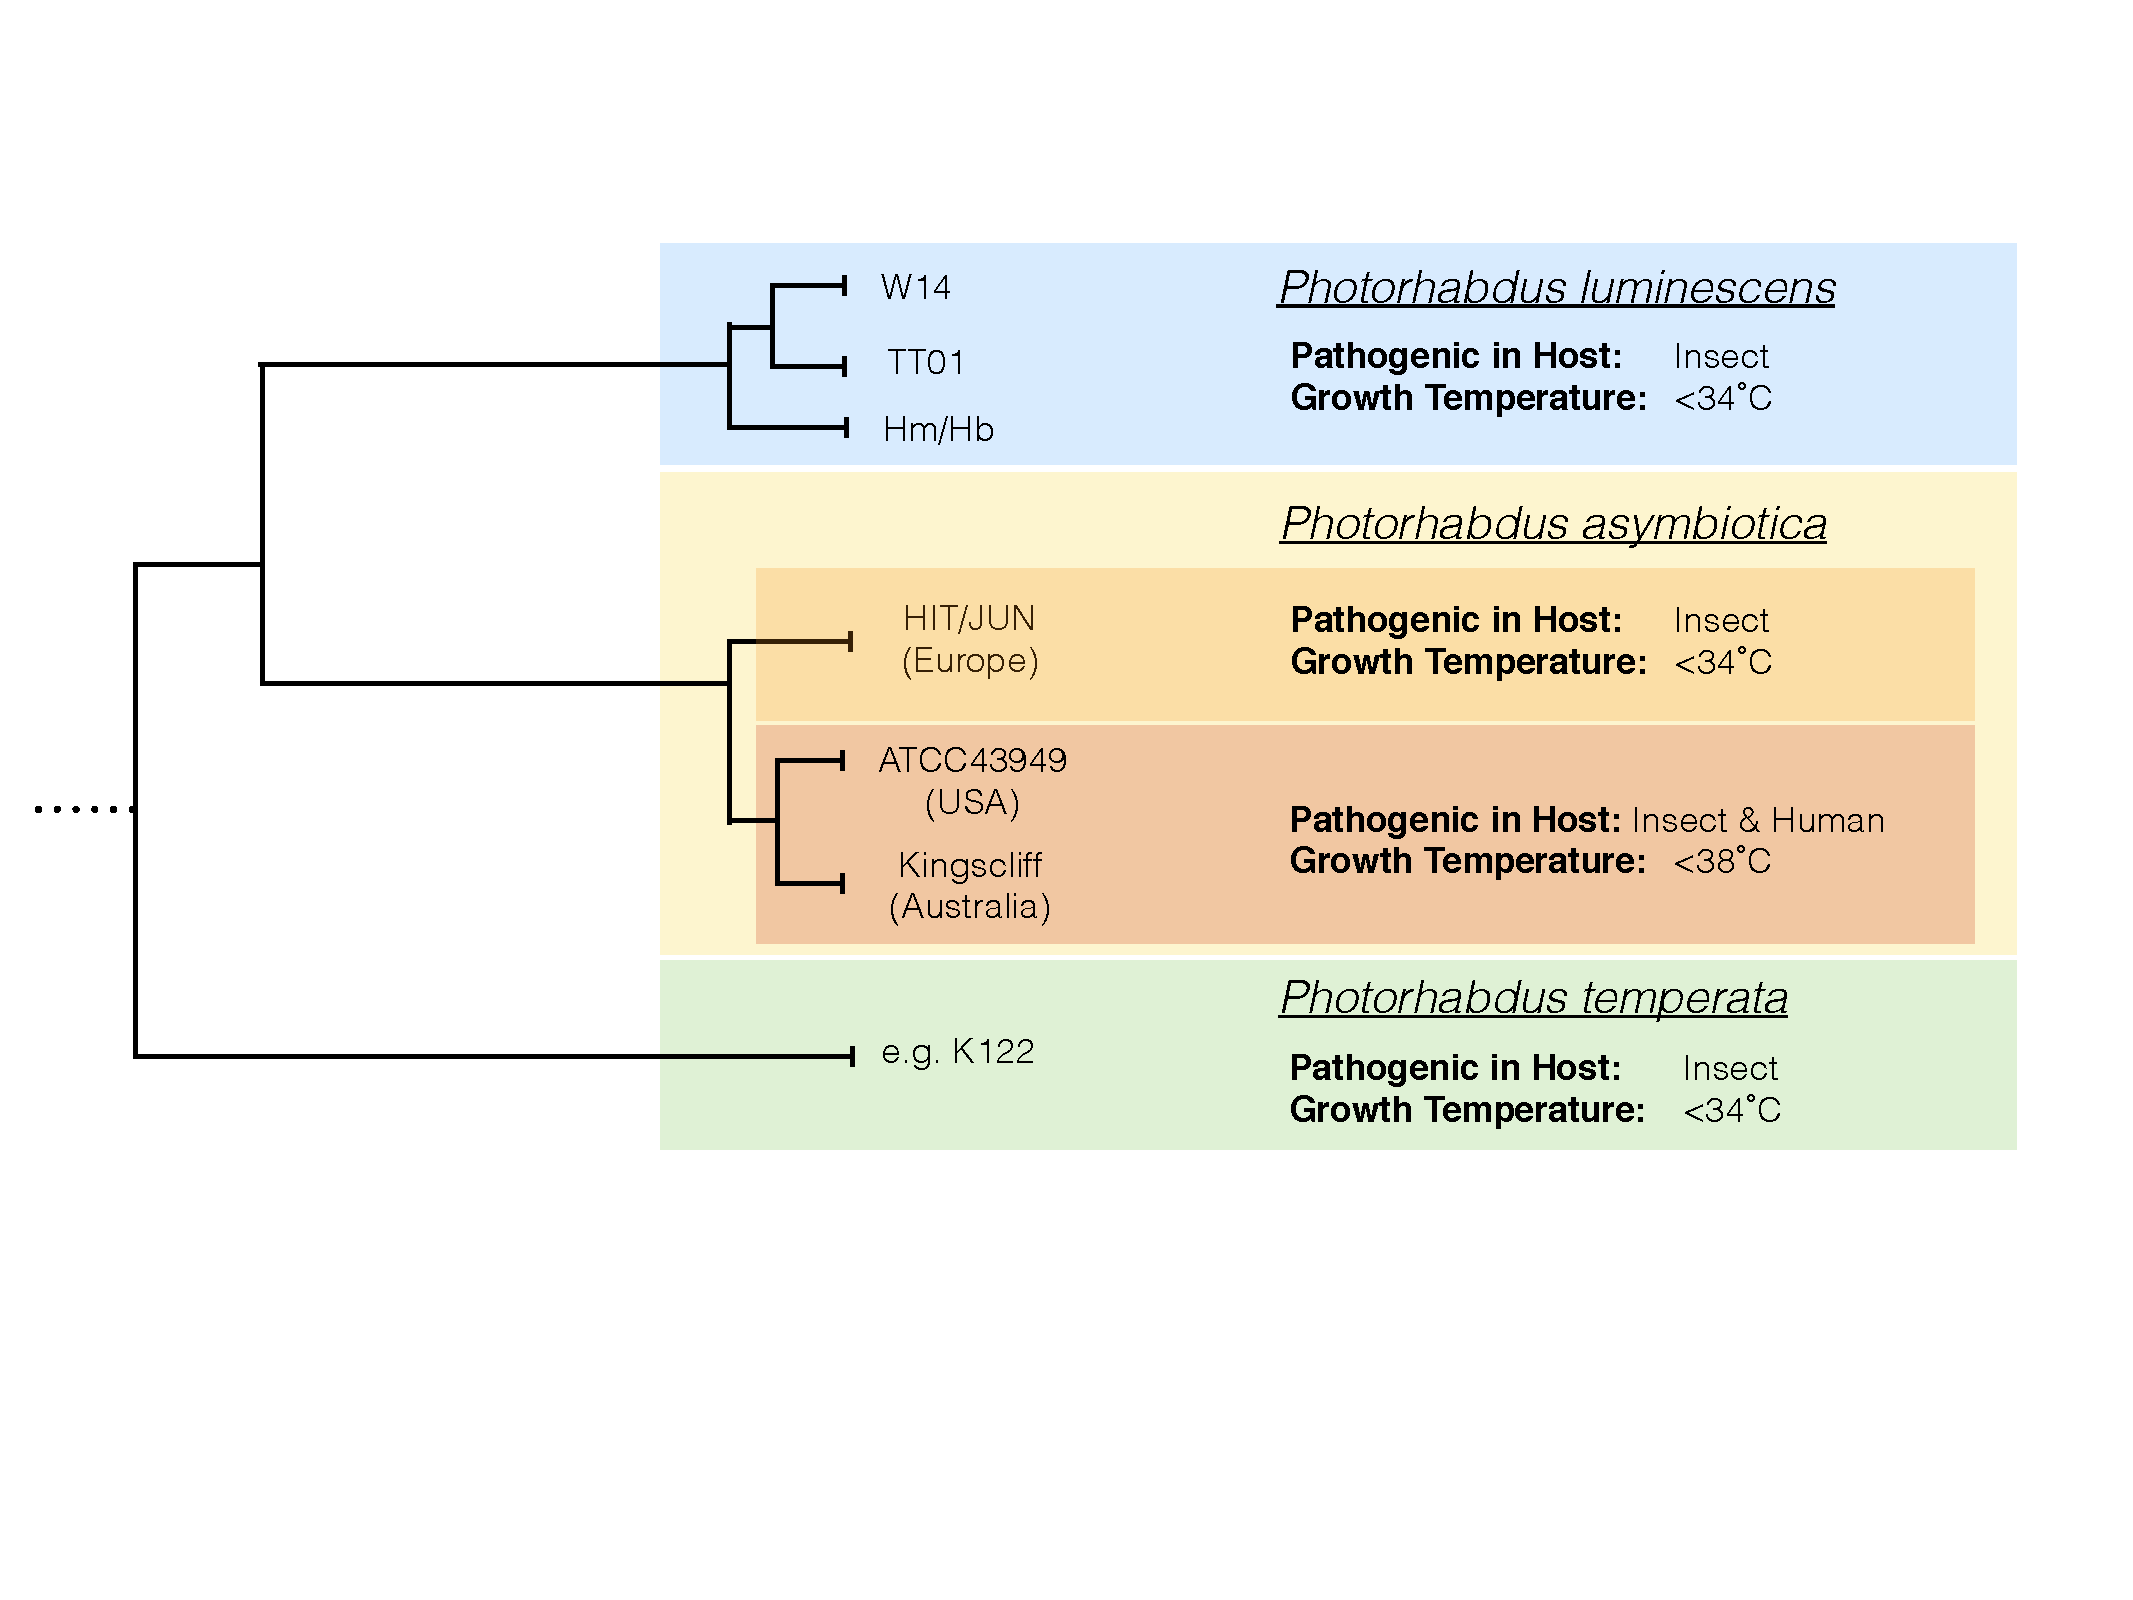
\includegraphics[width=\textwidth, clip, trim={50 180 50 110}]{/Users/joehealey/Documents/Warwick/PhD/Thesis/chapters/intro/img/lineages.pdf}
    \captionsetup{singlelinecheck=off, justification=justified, font=footnotesize, aboveskip=0pt}
    \caption[Schematic diagram of \emph{Photorhabdus} lineages]{\textsc{\normalsize A schematic diagram depicting the subclades within the \emph{Photorhabdus} genus.}\vspace{0.1cm}\newline Not drawn to scale. The schematic shows the host ranges and thermotolerance of the archetypical species within the \emph{Photorhabdus} genus, with some exemplar strains. Adapted from \citep{Waterfield2009}, and reproduced from my own Masters thesis ``\emph{Photorhabdus asymbiotica} as a Model Organism for Understanding Emerging Human Pathogens".}\label{lineages}
\end{figure}

These differences in genetic content and pathogenicity notwithstanding, all \emph{Photorhabdus} strains are obligately associated with \emph{Heterorhabditid} nematodes (see upcoming \vref{lifecycle} for a detailed explanation). Consequently, all strains must maintain the capability of associating with the host. These interactions are undoubtedly extremely complex, requiring all manner of genetic components as well as transcriptional and translational epigenetic regulation, and the molecular basis for this symbiosis is still yet to be fully understood, though some progress has been made. \Pa{} is known to exhibit a kind of phase variance, and previous studies have demonstrated that secondary phase bacteria are unable to support symbiosis, being termed ``symbiosis-deficient"; though \Pa{} phase variance appears to differ somewhat from that of other bacteria in being uni-directional \citep{Ffrench-Constant2003}. In the process of bioconversion of an infected insect, late phase \Pa{} have been shown to produce an array of secreted proteins such as proteases, toxins, and antimicrobials, to degrade the cadavers, and ward off non-\emph{Photorhabdus} competition (be it from other microbes, or from scavenging insects) \citep{Daborn2001a,Baur1998}. 

Thus, every \Pa{} strain studied to date maintains within its genome, all the symbiosis factors required for association with the nematode vector. This includes any `standard' genetic determinants, but also any regulatory and epigenetic mechanisms. All the strains also maintain virulence factors and bioconversion enzymes required to cause lethal infection and biomass conversion of an insect prey. In the case of \Pasy, they must do this in spite of a reduced genome size (though with the gain of one or more plasmids), as well as harbour all the necessary genetic apparatuses to confer infectiousness in higher order homeotherms (including, but not limited to: thermotolerance, adaptive immune resistance/evasion, facultative intracellularity). This has given rise to the hypothesis that rather than maintain a repertoire of `anti-insect' and `anti-mammalian' virulence factors etc., that instead, the virulence factors it has are efficacious against cell types from both organisms \citep{Waterfield2004a}.

\subsection{A biological `box of tricks'}
There are a number of extremely interesting and unusual aspects of \Pa{} cellular biochemistry and physiology that make it a fascinating study organism. A member of the \emph{Enterobacteriaceae}, \Pa{} is a motile, Gram negative rod shaped Gammaproteobacterium, which is partially what gives it its name: ``rhabdus" from the Greek, ``\emph{rh\'abdos}`` - ``rod" or ``wand". The former portion of its name is derived from perhaps its most striking characteristic: bioluminescence (Greek: ``\emph{ph\^os}'' - light). \Pa{} is still the only known terrestrial bacterium that exhibits bioluminescence, and does so through possession of the full \emph{luxCDABE} operon \citep{Peat2010,Clarke2008a,Farmer1989,Gerrard2003}. Why \Pa{} has maintained the operon is still a mystery, but hypotheses include use as a signalling mechanism, similar to its marine counterparts, in symbiosis (signalling to the nematode that a cadaver is populated for instance), or possibly as a virulence mechanism to deal with oxygen free radicals and enhance survival - however there is sparse evidence for these theories, and valid counters to all of them \citep{Waterfield2009}. Nevertheless, it has lead to interesting anecdotes about a phenomenon observed during the American Civil War, known as ``Angel's Glow", which has made its way in to some popular media including being covered in the well-known educational magazine ``Mental Floss" \citep{Durham2001,Soniak2012}. The phenomenon observed that soldiers who were wounded in the conflict, had a greater average survival rate if their wounds glowed. The subsequent rationale for this is that their wounds may have been infected with \Pa, which produces a myriad of antimicrobial compounds and toxins, killing off competition, including more virulent human pathogens that would have otherwise killed the individual.

The last point is another profoundly interesting and important aspect of \Pa{} biology. At the time of sequencing, it was discovered that \Pa{} has a greater proportion of its genome dedicated to secondary metabolite and toxin production than any other bacterium - including the model for secondary metabolite production, \emph{Streptomyces} (6\% vs. 3.8\%) \citep{Waterfield2009,Duchaud2003}. Among these secondary metabolites, a stilbene compound has been previously identified, \emph{3,5-Dihydroxy-4-isopropyl-trans-stilbene}, which, for a long while, \Pa{} was thought to be unique in being the only non-Plant organism known to produce it \citep{Joyce2008} - more recently it has also been detected as an \emph{Bacillus} metabolite too \citep{Kumar2013}. The compound itself has been shown to be a potent and broad range antimicrobial \citep{Hu2000}.
Consequently, the burgeoning field of `bio-prospecting' (`genome mining') \citep{Shi2018}, has begun to turn it's attention to \Pa{} as a source of novel compounds - particularly important as we continue to try and combat the threat of antimicrobial resistance \citep{Orozco2016}, and helpful as \Pa{} researchers, as it is leading to an increase in the number of available genomes and roles for many of the unknown genes. This will no doubt continue to affirm \emph{Photorhabdus}' place within the biotechnology world, complementing the exploitation which is already underway of the \emph{lux} operon, and the organism itself for biopesticides - and, we hope, the PVCs in due course.

\subsection{The life cycle of a pathogen and mutualist}\label{lifecycle}
\Pa{} is an obligate pathogen and symbiont \citep{Ffrench-Constant2003}. Much of the research interest in the organism to date has been specifically because of this unusual life style. There are abundant examples of symbiotic microorganisms and pathogenic organisms, but very few where both lifestyles are found to be exhibited by a single organism. Trying to unravel the complex molecular basis for this is a huge task, making \Pa{} an unusual and valuable emerging model.

\Pa{} is a seemingly ubiquitous soil dwelling bacterium, having been isolated from all over the world, though most commonly near coastlines. However, it is not thought to survive exposed in the soil by itself. Instead, it is found in mutualistic symbiosis with entomopathogenic soil nematodes, specifically members of the \emph{Heterorhabditidae}. In fact, such is the specificity of this mutualism, that different nematode species are known to harbour only particular bacterial species - the closely related \emph{Xenorhabdus} are associated with \emph{Steinernema} nematodes instead, for example \citep{Chaston2011}. The `bacterium-nematode complex' has potent demonstrated lethality against members of the \emph{Lepidoptera}, \emph{Coleoptera}, \emph{Hymenoptera}, and \emph{Dictyoptera} \citep{Naidoo2015}, and has been used for many years now as a biopesticide \citep{Waterfield2009}. In the soil, the bacteria are associated with the so-called ``Infective Juvenile" (IJ) (which is developmentally equivalent to the ``Dauer juvenile" of \emph{Caenorhabditis elegans}) stage of the nematode host, which is free living and actively seeking insects to infect/parasitise. 

\begin{figure}[h]
    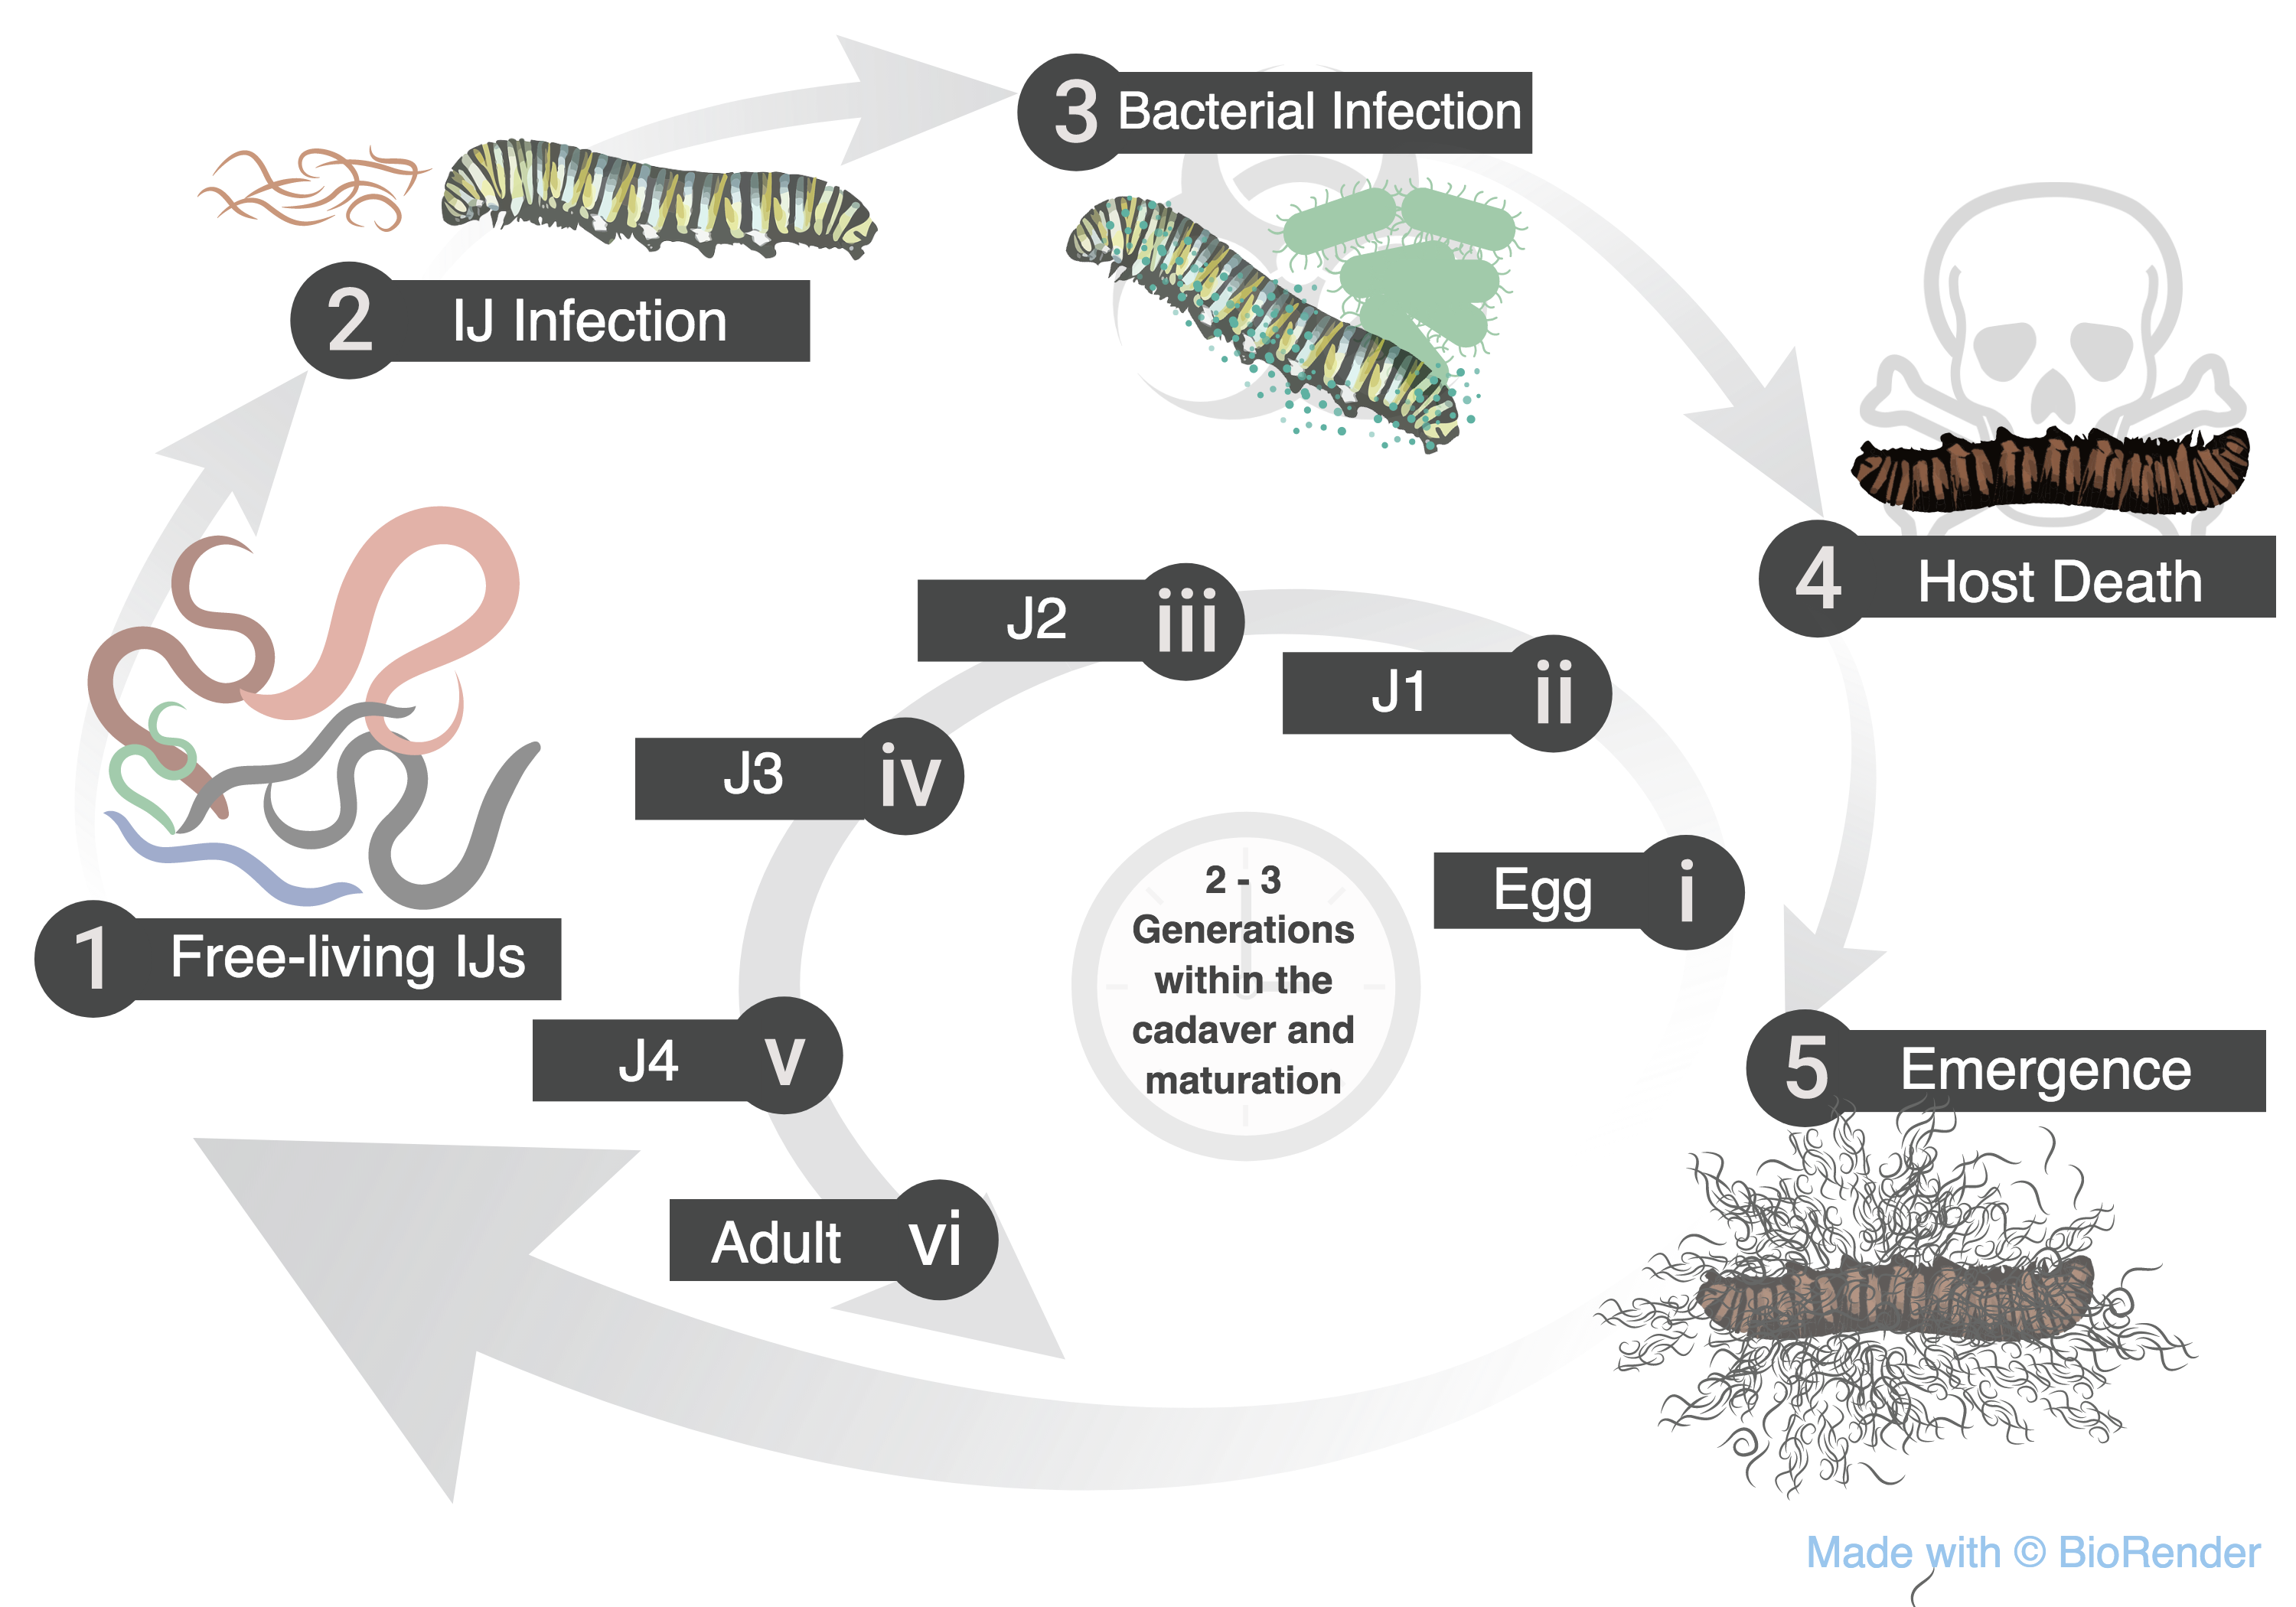
\includegraphics[width=\textwidth, clip, trim={0 25 0 0}]{/Users/joehealey/Documents/Warwick/PhD/Thesis/chapters/intro/img/lifecycle.png}
    \captionsetup{singlelinecheck=off, justification=justified, font=footnotesize, aboveskip=10pt}
    \caption[Diagram of \emph{Photorhabdus} and \emph{Heterorhabditid} nematode infection cycle]{\textsc{\normalsize The infection lifecycle of the Entomopathogenic Nematode complex.}\vspace{0.1cm}\newline
\textbf{(1)} The free living ``Infective Juveniles'' (IJs) in the soil seek out a new insect host to prey on. \textbf{(2)} IJs ingress in to the insect prey either through natural openings or boring through the cuticle. \textbf{(3)} \emph{Photorhabdus} bacteria are regurgitated by the EPN in to the open blood system of the insect (hemocoel). \textbf{(4)} The bacteria reproduce and express virulence factors to kill the prey in a matter of hours. \textbf{(5)} Bio-conversion of the cadaver biomass in to additional bacteria provides a food source for the continued reproduction of nematodes. \textbf{(i-vi)}) During replication on the cadaver, juvenile nematodes reach maturation and conduct their sexual reproduction phase. Millions of next generation IJs then leave the cadaver, reassociating with the bacteria to find the next prey insect. Adapted from \url{http://www.giabr.gd.cn/kxcb/kpdt/201405/t20140516_234014.html}, and in turn \citep{Ffrench-Constant2003}}
    
 \label{lifecyclefig}
\end{figure}

As \vref{lifecyclefig} shows, the cycle begins with free-living Infective Juvenile nematodes in the soil. The IJs are associated with their \emph{Photorhabdus} symbiotes, where the bacteria reside in the lumen of the nematode gut. Conversely, in the \emph{Xenorhabdus-Stiernema} complex, the bacteria are relegated to quiescent growth in a specialised region of the intestine known as the `receptacle'. IJs are a specialised alternative third developmental stage which are non-feeding, self-fertile hermaphrodites, with increased resilience to environmental stresses (by retaining an additional cuticle layer \citep{Ciche2003a}). IJs seek out prey insects within the soil to parasitise, and enter the organisms open circulatory system (or ``hemocoel'') via natural openings such as the spiracles (breathing tubes), mouth or anus. Alternatively, the nematodes bear a sharp tooth-like structure at the mouth which they can use to bore through the cuticle of the organism. Once inside, the nematodes regurgitate their bacterial `payload', which is typically less than 200 individual cells, speaking to the potency of the entomopathogenic activity of \emph{Photorhabdus}, which then employ sophisticated molecular tools to evade the immune response and establish an infection. The regurgitation and triggering of developmental processes for the nematode are induced by compounds within the insect hemolymph (blood) \citep{Ciche2003a}. Interestingly, the same paper by Ciche and colleagues showed that Grace's insect medium could not replicate this effect, suggesting that it is only very specific compounds involved in the process which are not reproduced in artificial media, though these compounds could not be identified specifically. Over the course of the next $\approx$36 hours, the IJs developmental switch, brought about by the insect environment, triggers feeding behaviour. The bacteraemia is lethal to the host insect, due to rapid proliferation and production of many exoenzymes and virulence factors. The bacteria therefore digest and bioconvert the cadaver, and the nematodes feed on the new bacterial biomass. Some of the ingested bacteria adhere to the nematode intestine and invade the rectal gland cells, restoring the EPN complex. While growing and maturing on the insect cadaver, the nematodes can complete their maturation to adults, having been larval juveniles up to this point. Their development to adults also leads to a dioecious stage, rather than the hermaphroditic one seen in the IJs, meaning that the nematodes can undertake sexual reproduction. Once the cadaver is exhausted, the EPN complexes vacate the site and go off in search of fresh prey, repeating the cycle.

There are a number of theories suggesting a basis for the control of symbiosis and the switch to pathogenicity (though a full review is beyond the scope and need of this thesis), including the use of the \emph{lux} operon as mentioned earlier, and recent studies have shown that many of the secondary metabolites that \Pa{} produces have roles in this mechanism. It has been observed that mutants in \emph{relA} and \emph{spoT}, which are both ppGpp alarmone synthases, become deficient in secondary metabolism and in symbiosis, but not in virulence \citep{Bager2016}. Mutants in the malate dehydrogenase enzyme (\emph{mdh}), exhibited similar behaviour, with no effect on virulence, but becoming incapable of mutualism (and unable to produce light, pigments, and the previously mentioned stilbene compound; all of which are hallmarks of post-exponential phase secondary metabolism). \emph{mdh} is a central enzyme in the Krebs' Cycle, implicating it in both central and secondary metabolism \citep{Lango2010}. Similarly, mutants in \emph{hfq}, a global post-transcriptional regulator that is widespread in bacteria demonstrated complete abolishment of all known secondary metabolite production, and a concomitant failure to associate with the nematode vector \citep{Tobias2016}. Large-scale lifestyle decisions, such as sporulation in \emph{Bacillus}, a process thought to involve as much as half of the genome, may be analogous. Certainly, there are similarities in that both processes require a functional Krebs' cycle \citep{Stephens1998}, and so it seems likely that a complex process such as symbiosis could also involve a significant proportion of the genome. It is probable, therefore, that any or all of the aforementioned theories are true, and that there are a vast number of pathways working together to fettle and control the symbiosis and pathogenicity process.

%\section{Toxins and Virulence Factors of \Pa}
%As this thesis primarily concerns a toxin system of \emph{Photorhabdus}, a little more time will now be dedicated to discussing the dizzying array of toxins/virulence factors which the bacteria puts to use, before discussing the PVCs specifically. Mounting information on the structure and biological activity of many of the toxins from \emph{Photorhabdus} is only serving to reinforce the earlier assertion that the genus harbours a greater number and diversity of toxic entities than seen in any other genus of microorganism to date, and thus there are interesting evolutionary pressures acting to maintain what, would at first glance, appear to be a genome of high redundancy \citep{Richard2014a}.
%
%\subsection{Mcf}
%\subsection{Pir}
%\todo[inline]{populate this section}
%
%\subsection{The ``Tc" Toxins}
%One of the earliest discoveries, which has spurred a significant amount of \emph{Photorhabdus} research, was the identification of the orally active ``Tc" system \citep{Bowen1998}. Taking their name literally from ``Toxin Complexes", the Tc's are formed from 3 separate components - TcA, TcB and TcC. The structure, which was recently resolved in atomic detail \citep{Meusch2014}, shows that TcA multimerises in to a striking, inverted bulb-like, or vase shape, and the whole complex is on the order of a megadalton. The pentameric TcA complex is a staggeringly elaborate cell surface binding and payload ejection system. An entropic spring chain of amino acids that stretches across almost the length of the entire structure keeps it poised such that upon binding to the cell an outer shell is retracted, revealing an extended helical central channel which is forced into the membrane, creating a pore. TcB and TcC sit atop the `vase' like structure forming a so-called ``cocoon", comprised mostly of a $\beta$ sheet cage-like structure with a hollow interior. In early study, it was observed that the TcA gene could be expressed alone, but TcB and TcC had to be expressed together, and only when all 3 components were reconstituted together was oral toxicity restored \citep{Richard2014a, Waterfield2001z, Sergeant2003}.  The toxic moiety of this enormous complex is contained within the TcC protein, but interestingly, the protein is not dedicated to just being a toxin, forming half of the `cocoon' that was just mentioned. In fact, the TcC C-terminus is cleaved off by the TcB, meaning that both perform catalytic as well as structural roles. Physicochemical properties of the interior of the cocoon mean that the cleaved C-terminus moves in to the lumen of the pre-pore within the centre of the TcA pentamer. Upon binding to the cell, the enormous conformational change that occurs in the TcA, penetrating the membrane, allows the toxic subunit free passage to the cytosol. Meusch and colleagues make the interesting observation that TcC are hyper-variable, meaning that there is the potential to delivery a diversity of toxin `payloads' \citep{Meusch2014}. It has also been noted that the \Plum{} TcB/C complex shares only around 56\% sequence identity with the homologous structures in \emph{Yersinia entomophaga}, despite elaborating almost identical tertiary and quaternary structures \citep{Richard2014a}. This diversity of sequence, yet conservation of structure/function, has lead to these complexes being termed `polymorphic toxin systems', along with the PVCs \citep{Zhang2012a}. These systems are characteristically highly recombinant, particularly in the types and modes of actions of their payloads, and this is an important point worth bearing in mind for much of this thesis. Under this nomenclature, both the Tcs and the PVCs are classified with the type II, V, VI and VII secretion systems, among others.
%
%
%This just goes to show the ingenuity \Pa{} (and many other related bacteria) are exhibiting when creating highly effective and staggeringly complex toxin systems - a fact that will be all the more apparent shortly when the PVCs are introduced fully.

\section{The \Pa{} Virulence Cassette}
Not much is known for certain when it comes to the \Pa{} Virulence Cassettes, and even less has been published. To date, there has only been a single paper on the discovery and biology of the \emph{bona fide} PVCs \citep{Yang2006}. However, an increasing number of papers have appeared, particularly in the last $\approx$5 years, which have attempted to understand how PVCs `fit in', in a wider context, and have begun to speculate on the roles of various genes. While there is nothing wrong with this in principle, much of the biology is still lacking, and it is not always constructive to try and constrain a biological entity to fit within the criteria for different systems. With the rapid proliferation of structural data for analogous systems however, thanks in no small part to the advancements in cryo-electron microscopy for studying large macromolecular complexes, there has never been a better time to study fascinating structures such as these.

As these structures are complex, multipartite and still quite enigmatic, this section will serve as a `guided tour' through the various components of the PVC structures, as well as draw analogies against other, better characterised, related structures as it was understood before this project began, to help the reader understand the chapters to come. \vref{structbioinfo} will continue in this vein, in the context of what has been learnt since, with the advantages of more complete databases and a better biological understanding, to fill in some of the gaps.

\subsection{Discovery of the PVCs}
Upon sequencing of the first \emph{Photorhabdus} genomes, the PVCs were identified as putative prophage regions the \Plum{} TT01 genome, in 4 tandem repeats which demonstrated unusual \% GC content. When a cosmid library was constructed from the \Pasy{} ATCC43949 genome, clones harbouring the operon for a particular PVC with the so-called `Pnf' (\emph{Photorhabdus} necrosis factor) cognate effector demonstrated high levels of injectable toxicity against whole insects - killing them in as little as 15 minutes, and earning them their name (``Virulence Cassettes") \citep{Yang2006, Waterfield2008}. It became apparent from these early experiments that the PVCs represented a novel kind of toxin delivery and translocation mechanism, and similar patterns of toxicity could be identified in other cosmid clones which bore other PVC variants. The Pnf effector of this particularly potent PVC, is homologous to the active site domain of cnf1 (Cytonecrosis Factor) of uropathogenic \emph{Eschericia coli}, and works in the same way, by activating Rho GTPase proteins inside the target cell, which leads to cytoskeleton depolymerisation \citep{Landraud2004, Buetow2001}. Further inspection showed this cosmid to contain what we have now come to recognise as a PVC, with its associated effector, and several more cosmids within the library were identified which contained various other PVCs. It was observed that a number of the cosmid-borne PVC operons are defective in some way, suggesting that the obtained colonies were those where the cosmids had been inactivated in some way such that they could be tolerated. This potential self-toxicity is the subject of \vref{regulation}.

The PVCs were able to be purified/enriched from the cosmid supernatants to identify the basis of the toxicity, using diethylaminoethyl-sepharose resins and upon imaging via electron microscope, sure enough, phage like structures were apparent in the samples. Subsequent immunogold staining using antibodies raised against the Pnf toxin showed that, when disrupted, the structures appeared to be loaded with the toxins. \vref{PVCems} shows some of the original microscopy, reproduced from the \cite{Yang2006} study, as well as some more recent micrographs from the lab and an ongoing collaboration with the Max Plank Institute in Dortmund, showing cleaner samples. Preliminary data from the collaboration with the Max-Planck Institute resolving the atomistic structure of the PVCs is now beginning to vindicate the many assumptions about the PVC architecture, biology and function.

\vspace{0.1cm}
\begin{figure}[h]
\centering
    \begin{subfigure}[b]{0.33\textwidth}
        \centering
        {%
\setlength{\fboxsep}{0pt}%
\setlength{\fboxrule}{1pt}%
        \fbox{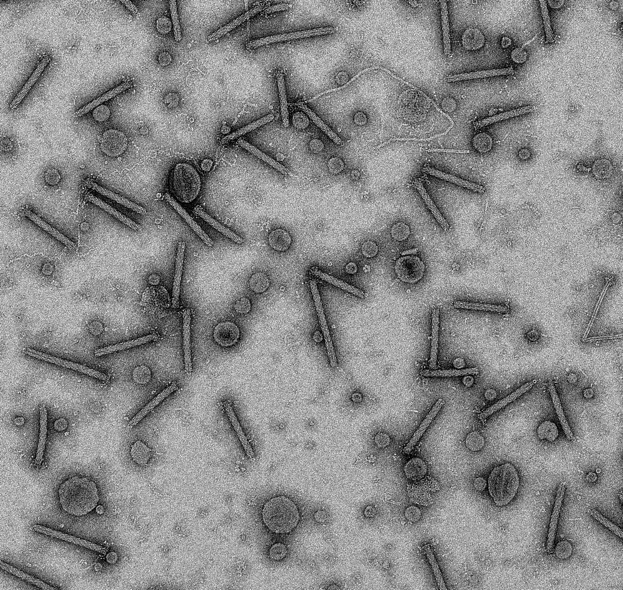
\includegraphics[width=\textwidth, trim={20 40.5 0 60}, clip]{/Users/joehealey/Documents/Warwick/PhD/Thesis/chapters/intro/img/PVCEM1.png}}
            }%
    \end{subfigure}%
    \begin{subfigure}[t]{0.33\textwidth}
        \centering
        {%
\setlength{\fboxsep}{0pt}%
\setlength{\fboxrule}{1pt}%
        \fbox{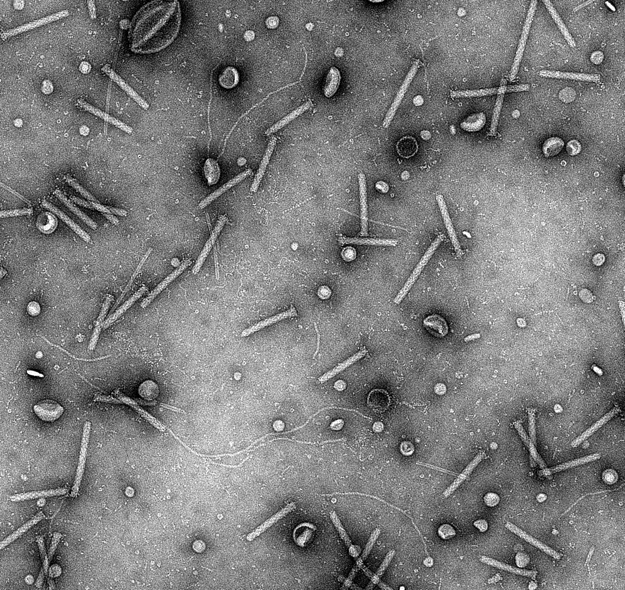
\includegraphics[width=\textwidth, trim={20 100 0 0}, clip]{/Users/joehealey/Documents/Warwick/PhD/Thesis/chapters/intro/img/PVCEM2.png}}
        }%
        \end{subfigure}%
    \begin{subfigure}[t]{0.33\textwidth}
        \centering
        {%
\setlength{\fboxsep}{0pt}%
\setlength{\fboxrule}{1pt}%
        \fbox{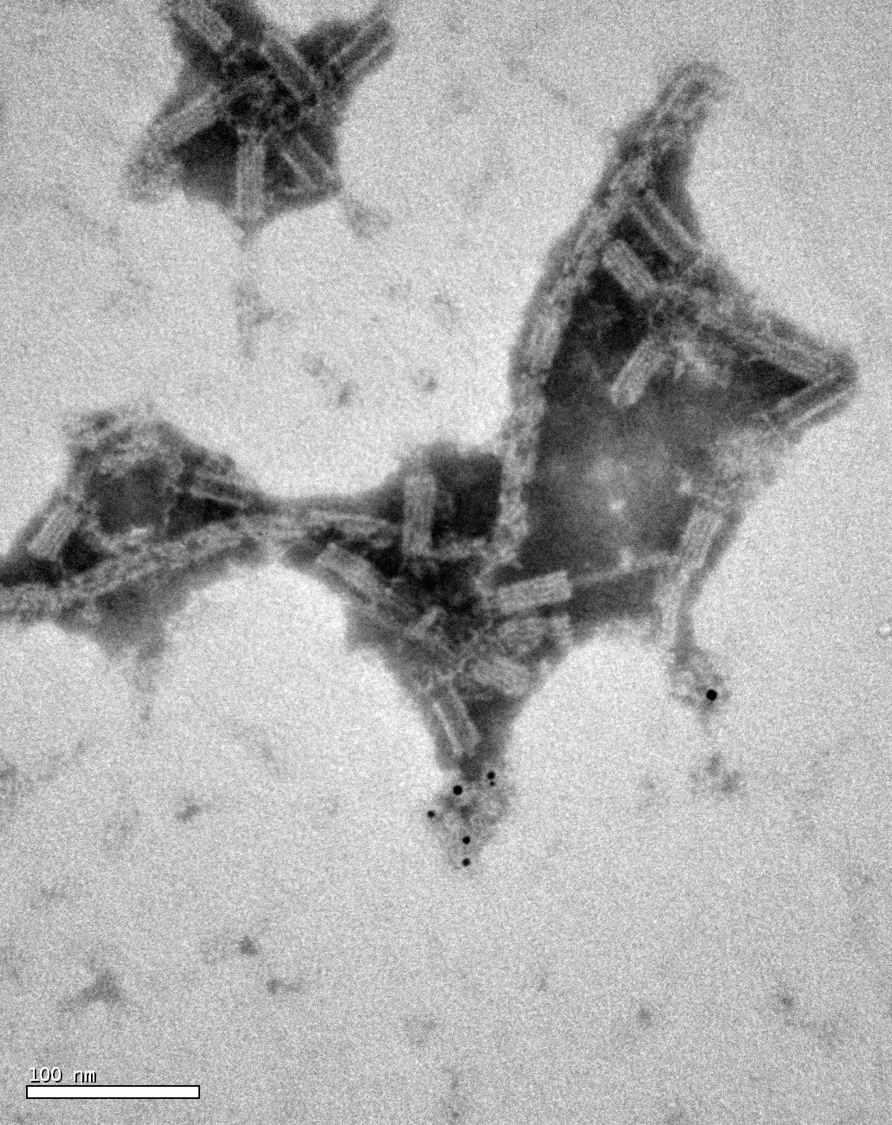
\includegraphics[width=\textwidth, trim={0 120 40 165.5 }, clip]{/Users/joehealey/Documents/Warwick/PhD/Thesis/chapters/intro/img/PVCEM3.png}}
        }%
    \end{subfigure}%

\captionsetup{singlelinecheck=off, justification=justified, font=footnotesize, aboveskip=10pt}
\caption[PVC Electron Micrographs]{\textsc{\normalsize A selection of electron micrographs of the PVCs.}\vspace{0.1cm} \newline A selection of micrographs are shown here revealing their caudate structure and the resemblance to other contractile tail systems. The left and centre panels show more recent, but unpublished data from an ongoing collaboration with the Max Planck Institute at Dortmund, purified via Cesium Chloride buoyant density gradient ultracentrifugation. The right hand panel shows one of the earliest images of the PVCs ever obtained, via diethylaminoethyl sepharose resin elution (the white mass in the background). The black dots in the bottom-center of this panel correspond to immunogold antibody staining against the payload molecules released from the syringes.}
\label{PVCems}
\end{figure}


\subsection{\Pa{} is a PVC addict}
A single PVC is a remarkable biological entity. However, \emph{Photorhabdus} has chosen not to stop here. Within the genomes studied to date, there are as many as 6 distinct PVC operons, each with 1 or more associated toxin effectors, in any single genome. The fact that each one has a hallmark effector or effectors has been used since their discovery to delineate which PVC is under discussion \citep{Yang2006} - with some exceptions. In several cases, the PVCs were simply named for their positions in the genome. Specifically, in \Plum{} TT01, the 4 tandem PVCs mentioned in the previous section were simply named ``Unit1", ``Unit2", ``Unit3", and ``Unit4". In \Pasy {} genomes, there is also a distinct ``Unit1", but confusingly, it is not most homologous to the ``Unit1"s of \Plum, being in fact, primarily orthologous to the \Plum{} TT01 ``Unit 4".

With this in mind, this is an ideal moment to briefly explain the nomenclature that will be used throughout this thesis when referring to the PVCs. The PVC with the cognate Pnf toxin that was mentioned in the previous section will be used as an example. In order to denote each PVC, the nomenclature ``PVCPnf" will be used. Where a distinction between inter-strain variants of the same operon is required, this will be followed by the strain name itself, as in: ``PVCPnf ATCC43949" or ``PVCPnf Kingscliff". Furthermore, when a specific gene is under discussion, ``PVCPnf" will be followed by the numerical identifier for that gene; so for the first protein of the \Pasy{} ATCC43949 strain Pnf operon, the nomenclature will become: ``PVCPnf1 ATCC43949". In cases where this thesis refers to just a specific locus, across all operons, the terminology will simply be ``PVC1" - i.e. the first locus, in all operons syntenically.

\vref{pvcvariants} demonstrates the variants from the \Plum{} TT01 and \Pasy{} genomes. The existence of phage-like contractile tails in a myriad of genomes has now been demonstrated, however, \emph{Photorhabdus} appears to remain somewhat unique, in that no other organisms have been found, so far, which harbour so many forms of the same structure in a single genome. Even if one examines \emph{Xenorhabdus} strains, which are as closely related as it is possible to be outside of the immediate \emph{Photorhabdus} genus, it is only possible to identify single copies of PVC-like operons.

\begin{figure}[p]
	\thisfloatpagestyle{IHA-fancy-style}
	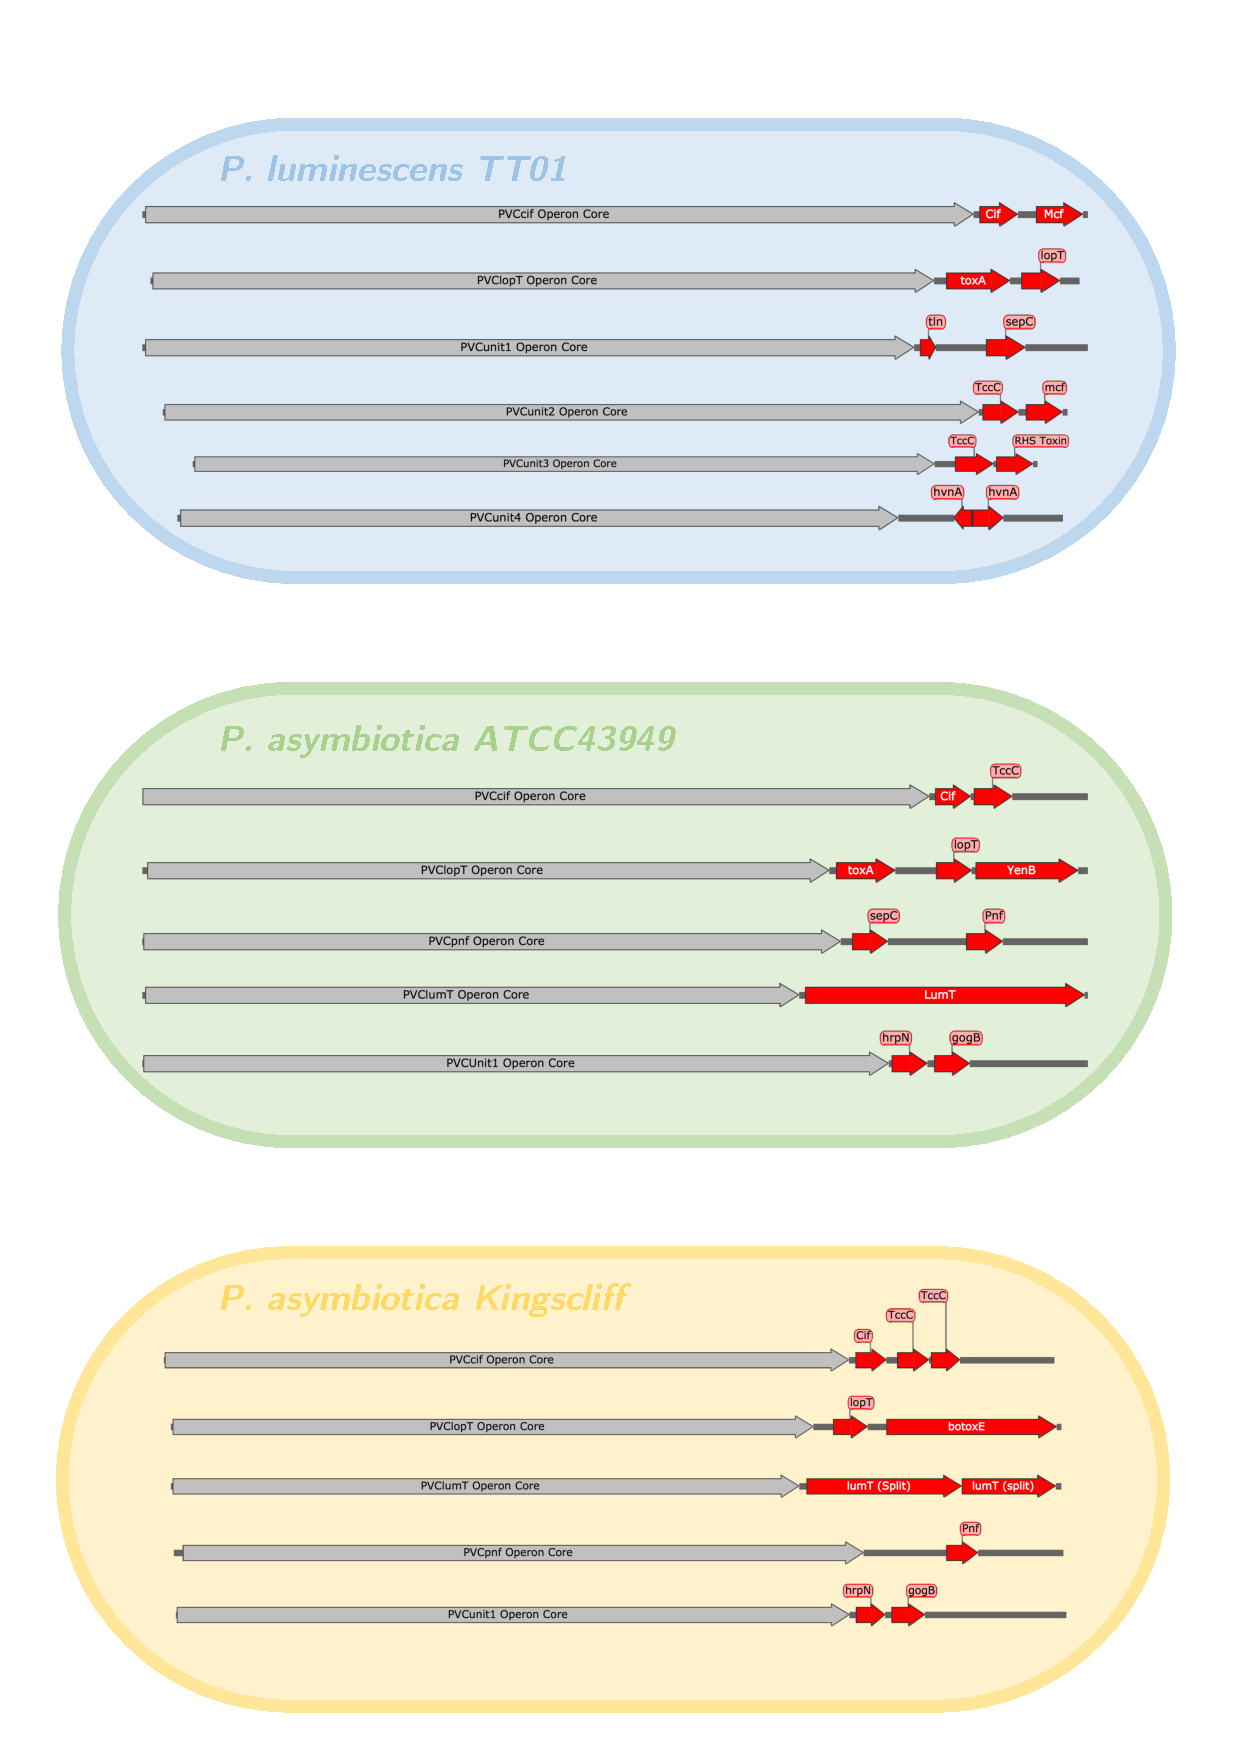
\includegraphics[width=\linewidth, clip, trim={25 10 26 55}]{/Users/joehealey/Documents/Warwick/PhD/Thesis/chapters/intro/img/hostofhostsfig.pdf}
	\captionsetup{singlelinecheck=off, justification=justified, font=footnotesize, aboveskip=5pt}
	\caption[Schematic of PVC variants across 3 \emph{Photorhabdus} genomes]{\textsc{\normalsize The PVC variants found in 3 \emph{Photorhabdus} genomes.}\vspace{0.1cm} \newline A schematic of the variant forms of PVCs found in the 3 different genomes this thesis will focus on. The operon core is denoted in a single grey arrow, and the diverse effector proteins which distinguish the operons are identified in red. Individual operons are to scale, however the scale between operons is not identical; they are all approximately 23 - 25 kbp.}
	\label{pvcvariants}
\end{figure}

\todo[inline]{Add a table of nomenclature}

Naturally, this leads to questions about how and why \emph{Photorhabdus} is able to maintain so many copies of operons which have a high degree of internal and inter-operon paralogy. Conventional wisdom would suggest that at least 1 of these extra operons might drift to the point of removal/pseudogenicity. For certain, there are substantial genetic differences between different PVCs, and drift has most likely played a part in this, but nevertheless they persist, which suggests the selective pressure is sufficient on each PVC to maintain them. There are a few speculative rationales that this could be the case. Firstly, it's possible that \emph{Photorhabdus}' life cycle is so competitive that any additional toxin systems of a net benefit to the organism, despite their high metabolic cost, with each fulfilling sufficiently different roles. This would further mesh with the observation that \emph{Photorhabdus} elaborates the largest repertoire of toxins known so far. An alternative idea however is that not all PVCs are evolved with a toxic effect in mind, and may have host modulatory effects - which will be covered in more detail in a later section. There is some preliminary evidence that different PVCs perform different roles, perhaps with toxicity to particular tissue/cell types, or responding to different environmental cues.

This almost paradoxical variability-yet-conservation is a recurring theme in this thesis, and is also useful for understanding any single one of the PVCs.



\subsection{PVCs as contractile nanomachines}
The initial electron microscopy, and homologies observed to R-type pyocins \citep{Ge2015}, the Antifeeding prophage \citep{Heymann2013},  and other prophage sequences, which have had their structures resolved or electron microscopy (EM) studies conducted, provided compelling evidence that the PVCs elaborated a similar caudate structure. Moreover, it has become increasingly apparent in recent years that the entire mechanism of `contractile machines' is an evolutionarily conserved structure which appears time and time again in nature - and not just in the form of prophages, which is what many of these devices have been mistaken for to date \citep{Kube2015a, Sarris2014, Brackmann2017}. In particular, in the Sarris et al. paper, contractile tail mechanisms of various forms have been demonstrated to be widespread with a remarkable diversity of functions, even in the Archaea. Much as the bacteriophage biosphere has become increasingly well understood to actively shape the bacterial biosphere, it is now becoming similarly apparent that phage-like structures will have had (and are having) a similarly decisive role in shaping ecosystems and evolution \citep{Richard2014a}. The following sections now detail the state of knowledge for the well studied cousins of PVCs; readers are also encouraged to look at the original Kube and Wendler, Taylor et al., and Sarris et al. papers for 2 excellent reviews from both a structural and genetic perspective, accordingly \citep{Kube2015a, Sarris2014, Taylor2018a}.

\subsubsection{Of PVCs and Phage}
Contractile tail nanomachines are typified by the bacteriophage order \emph{Caudovirales} (from the Latin: ``\emph{cauda}" - ``tail"), so it makes sense to start here. In particular, those of the \emph{Myoviridae} family, to which the well known model T4 phage belongs \citep{Ackermann1998}. Phages have been studied for over 100 years now, after their original discovery at the beginning of the 20th Century by F\'elix d'H\'erelle \citep{DHerelle1917}. d'H\'erelle is also credited with conceptualising phage therapy, which is becoming increasingly relevant again with the rise of antibiotic resistance.

The tail structures of the T4 bacteriophage were the first structures ever to be resolved by electron microscopic (EM) density reconstruction as far back as 1975 \citep{Amos1975}; and with the recent explosion of Cryo-EM data, and the so called ``Resolution Revolution" \citep{Kuhlbrandt2014}, we have a clearer understanding of these elegant and staggeringly complex macromolecular machines than ever before. The tail tube, capsid, and the intricate baseplate complex of T4 have now been solved to atomic or near atomic resolution \citep{Aksyuk2009, Kostyuchenko2003, Kostyuchenko2005, Fokine2004, Fokine2013, Rossmann2004, Taylor2016b, Lan2014}, and is probably the single most well studied structural entity. \vref{t4EMs} shows some of the actual micrographs of T4 collected to date, and \vref{t4structure} shows a collection of the now resolved structures reproduced from the literature. Even at a glance, its quite apparent that these entities share similar origins and architectures.

\vspace{0.1cm}
\begin{figure}[h]
\centering
    \begin{subfigure}[b]{0.41\textwidth}
        \centering
        {%
\setlength{\fboxsep}{0pt}%
\setlength{\fboxrule}{1pt}%
        \fbox{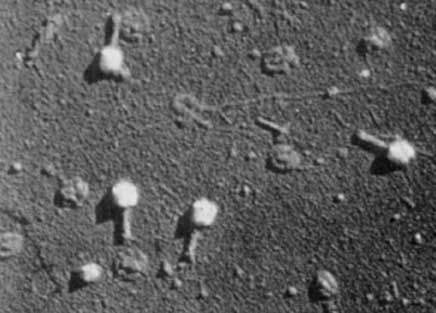
\includegraphics[width=\textwidth, trim={0 0 0 74.2}, clip]{/Users/joehealey/Documents/Warwick/PhD/Thesis/chapters/intro/img/EM_of_phage_T4.jpg}}
            }%
    \end{subfigure}%
        \begin{subfigure}[t]{0.16\textwidth}
        \centering
        {%
\setlength{\fboxsep}{0pt}%
\setlength{\fboxrule}{1pt}%
        \fbox{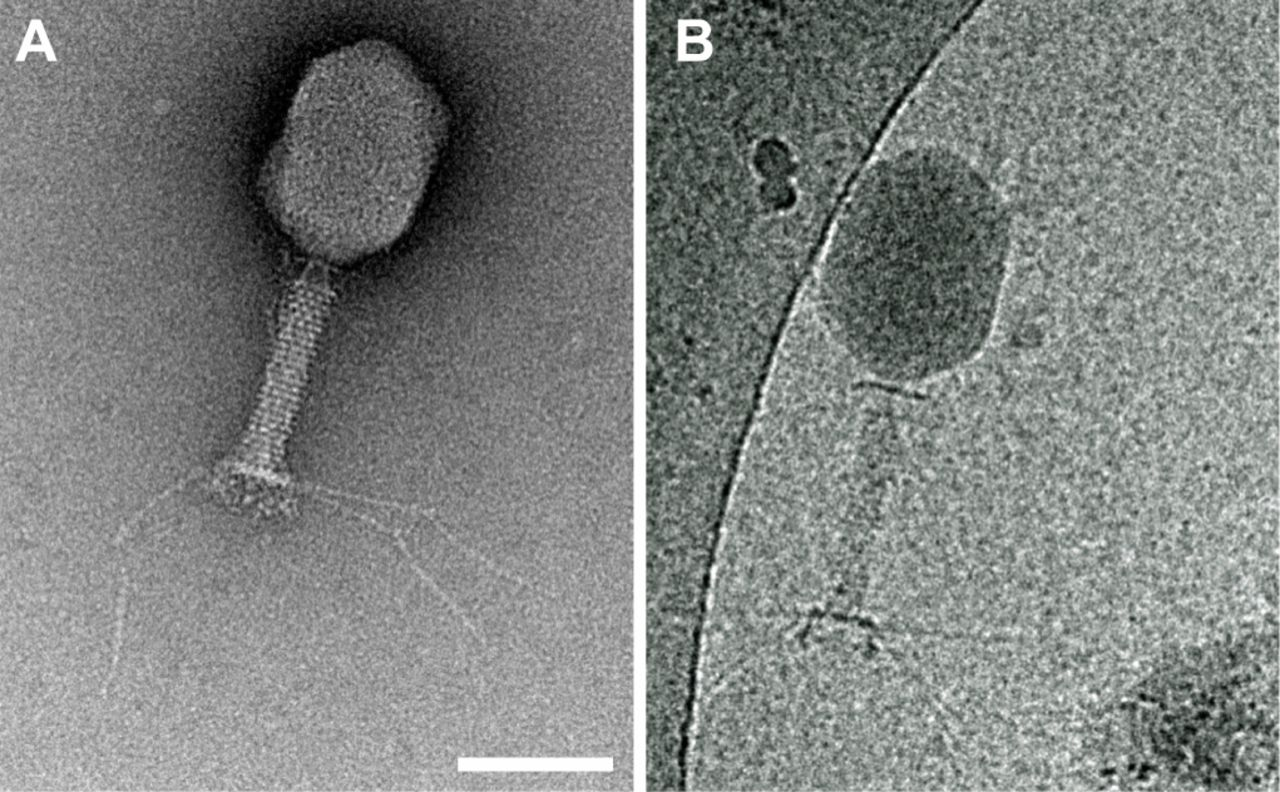
\includegraphics[width=\textwidth, trim={20 40 180 0  }, clip]{/Users/joehealey/Documents/Warwick/PhD/Thesis/chapters/intro/img/isEMdead.jpg}}
        }%
    \end{subfigure}%
    \begin{subfigure}[t]{0.41\textwidth}
        \centering
        {%
\setlength{\fboxsep}{0pt}%
\setlength{\fboxrule}{1pt}%
        \fbox{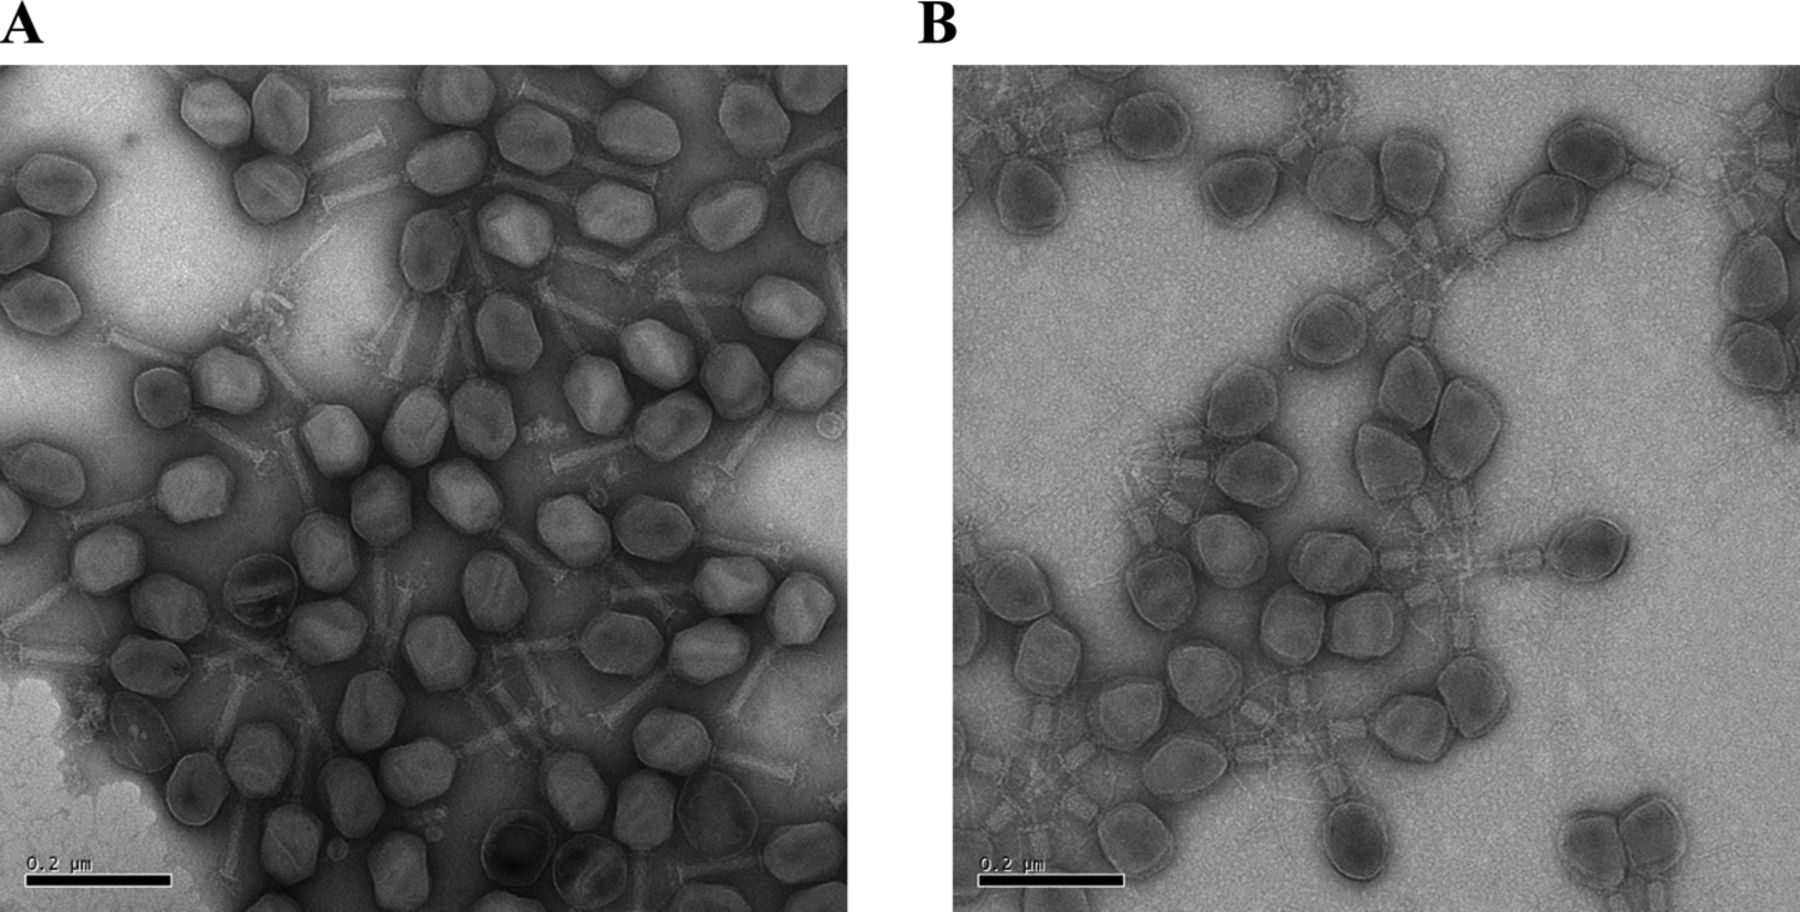
\includegraphics[width=\textwidth, trim={0 50 240 64}, clip]{/Users/joehealey/Documents/Warwick/PhD/Thesis/chapters/intro/img/EMlargescale.jpg}}
        }%
        \end{subfigure}%
	\captionsetup{singlelinecheck=off, justification=justified, font=footnotesize, aboveskip=10pt}
	\caption[Electron micrographs of Bacteriophage T4]{\textsc{\normalsize Electron Micrographs of T4 bacteriophage virions.}\vspace{0.1cm} \newline The left panel shows an early T4 phage micrograph from 1958, reproduced from \url{https://www.molbio.unige.ch/eng/about/history}. The centre panel shows a close up of the T4 phage, revealing the tail fibres, baseplate, capsid and tube in detail, reproduced from \cite{Knott2013}. The right hand panel shows a scaled up experiment, purifying virions for phage therapy, reproduced from \cite{Bourdin2014}.}
	\label{t4EMs}
\end{figure}


Despite their superficial resemblance in gross structure, PVCs appear considerably simpler than T4. As non-replicative entities, of course, the PVCs lack any machinery associated with this function (including the capsid packaging mechanism and replicative enzymes), but also differ quite substantially in structural proteins. PVC operons are typically around 25-30 kilobases in length, and usually encode approximately 25 proteins at most, whereas the T4 genome is nearly 170 kb, and encodes 289 proteins \citep{Miller2003}. 

From the very earliest annotations of the \emph{Photorhabdus} genomes, it was evident that there was shared homology for at least some of the genes in the operon. In particular, the inner and outer sheath proteins matched comparatively well, picking up annotations as gp19 (``gene product") proteins and major sheath proteins (gp18) respectively, whilst the majority of the operon remained as purely `hypothetical proteins'.  \vref{t4assemblyflowchart} shows how the many different subunits of the T4 sheath and baseplate complex together. The tail is comprised of 2 concentric hollow cylinders. The interior tube is comprised of stacked, helically offset, hexameric toroids of gp19. Similarly, the outer sheath of gp18 which provides the force for contraction has a helical hexameric cylindrical shape. \vref{t4sheaths} shows the helical nature of both the inner and outer sheaths well - a single ``protofilament'' of the outer gp18 is depicted in its extended (green) and contracted state (orange). In the relaxed state, the offset is approximately 17.2$^{\circ}$, and in the contracted state, this twist increases to 32.9$^{\circ}$ \citep{Kube2015a, Kostyuchenko2005, Leiman2004}. The exact mechanism of contraction for contractile tail systems is thought to be highly conserved, despite often significant differences in structure and sequence between structural homologues, and will be discussed for all the upcoming systems in \vref{mechanismofaction}.

There is evidence from heterologous expression of the analogous inner tubes of the Type 6 Secretion System (the Hcp1 protein) that the homohexameric toroids spontaneously self-assemble \citep{Ballister2008}, and that polymerisation begins from the gp27-gp5 spike tip complex (the so called ``baseplate hub complex'' \citep{Lan2014}) \citep{Kanamaru2002}. The gp18 homohexamers then also polymerise around the growing interior tube. The tail tube length is controlled by 3 further proteins, which have been identified as gp29, a ``tape-measure'' protein, and a tube terminator/cap protein complex of gp15 and gp3. The tail tube tape measure protein was identified by elongation and truncation experiments, with the actual tube length varying in accordance with the expansion of shrinking of the tape measure protein \citep{Abuladze1994}, and proteins serving similar roles have been identified in other contractile tail systems \citep{Katsura1987,Katsura1984, Isao1990}.

Despite having a couple of identifiable baseplate-like proteins, the PVCs appear to have radically reduced baseplates overall, though it must serve almost exactly the same purpose and function. It was possible to spot some assorted similarities to the gp6 baseplate component proteins, though in the absence of a full PVC structure, its still unclear exactly where these proteins will fit, and their exact role in the final structure. The T4 baseplate complex is exceedingly intricate, comprising some 18 different protein types (including the baseplate spike/hub, and the tail fibres), and roughly 57 separate protein molecules (some of which are, themselves, made up from multiple chains). As can be seen in \vref{t4assemblyflowchart} from \cite{Leiman2004}, 6 ``wedge" complexes are formed from a gp6-gp7-gp8-gp10-gp11-gp25-gp53 complex. Each of these 6 wedges then come together around the baseplate hub spike complex (gp27-gp5), itself comprised of 3 different proteins and at least 7 distinct chains. A further 12 proteins are added (6 each of gp9, and the tail fibres - gp12). Next, a heterodimeric toroid collar of gp48 and gp54 is then added to the apex of the dome shaped complex, similar to the keystone at the top of an arch. When scrutinising the T4 baseplate it perhaps makes sense that of all of the proteins for the PVCs to maintain detectable homology to, gp6 is the best hit, as it sits in close register to the collar and spike complex and is therefore a minimal component of the complex (depicted in light orange in \vref{wedgeformation}).

Though the PVC and T4 baseplates are likely to be substantially different in structure, the baseplate hubs/spike complexes appear to share more in common. Existing annotation attributes VgrG protein homology to the spike (which is associated with the T6SS - see \vref{t6ss}), rather than gp27-gp5, though these are extremely similar structures - among the most structurally conserved and easily identifiable amongst all caudate apparatuses despite often having as little as 13\% sequence identity \citep{Veesler2011, Leiman2009, Basler2015}. The T4 tail spike complex retains an Oligosaccharide/Oligonucleotide binding domain (``OB-fold" - a 5-stranded anti-parallel $\beta$-barrel \citep{Murzin1993}) and a lysozyme domain which appears to be lacking from the VgrG, instead being functionalised with assorted alternative enzymatic activities \citep{Pukatzki2007, Kanamaru2002} - an extensive discussion of VgrG will be saved for \vref{t6ss}.

Finally, the PVCs are thought to contain putative tail-fibre like genes, proposed to be for cell binding in the same manner as T4. So far, there appears to be no evidence of both long and short fibres as is the case in T4 however \citep{Bartual2010, Thomassen2003}. Again, the PVCs seem to elaborate a much simpler version of these analogous structures. The long tail fibres of T4 are comprised of 4 proteins: gp37 and gp34 form the main trimeric body of the fibre, but are separated in to a ``proximal" (thigh) and ``distal'' (shin) end by gp35 hinge (a so-called ``Knee cap" which induces a kink in the structure allowing them to fold away when in unfavourable infection conditions). At the upper end of the `shin' a trimer of gp36 is also present completing the knee joint \citep{Leiman2010}. The long tail fibres are anchored in to the baseplate structure by 6 trimer complexes of the gp9 protein (\vref{baseplateformation}). At the outermost edge of the dome, the 6 short tail fibres comprised of gp12 can be seen wreathing the edge in the folded state (in \vref{baseplateformation} they can be seen pinkish-purple; in \vref{extendedtailfibres} the short fibres can be seen in their extended state). The short tail fibres are known to be capable of folding correctly without the need for additional chaperones \citep{Leiman2010, Goldberg1997, Ali2003}. For the PVCs there appears to only be a single tail-fibre like gene, referred to as \emph{pvc13} due to its general syntenic location, and is the focus of \vref{tailfibres}, where a more detailed introduction to the tail fibre structure and proposed function can also be found. 

This review will not consider the assembly of the T4 capsid, as the PVCs do not contain analogous structure, but for an excellent all-round review of the full assembly of T4, see \cite{Yap2014a} and \cite{Leiman2010}.

%%%%%%%%%%%%%%%%%%%%%%%%%%%%%%

\begin{figure}[p]
\thisfloatpagestyle{IHA-fancy-style}
\centering
    \begin{subfigure}[h]{\textwidth}
        \centering                                                     % L   B    R   T
        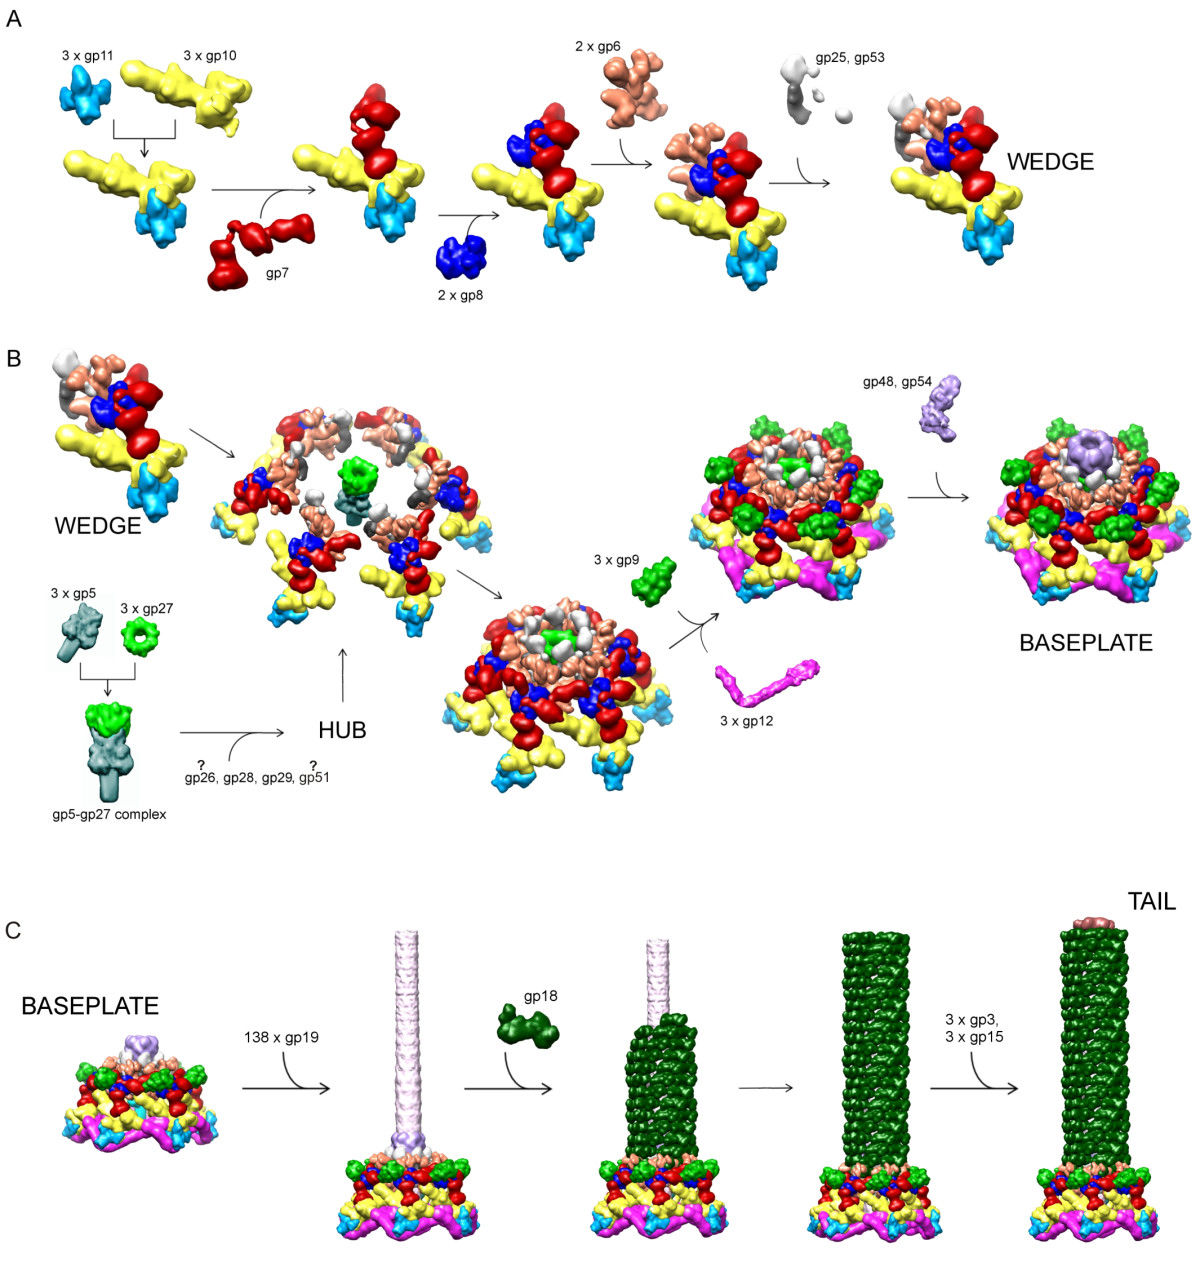
\includegraphics[width=\textwidth, trim={7 230 20 10}, clip]{/Users/joehealey/Documents/Warwick/PhD/Thesis/chapters/intro/img/t4assembly.jpg}
        \captionsetup{singlelinecheck=off, justification=centering, font=footnotesize, aboveskip=15pt, belowskip=10pt}
        \caption{}
        \label{wedgeformation}
    \end{subfigure}%

    \begin{subfigure}[h]{\textwidth}
        \centering
        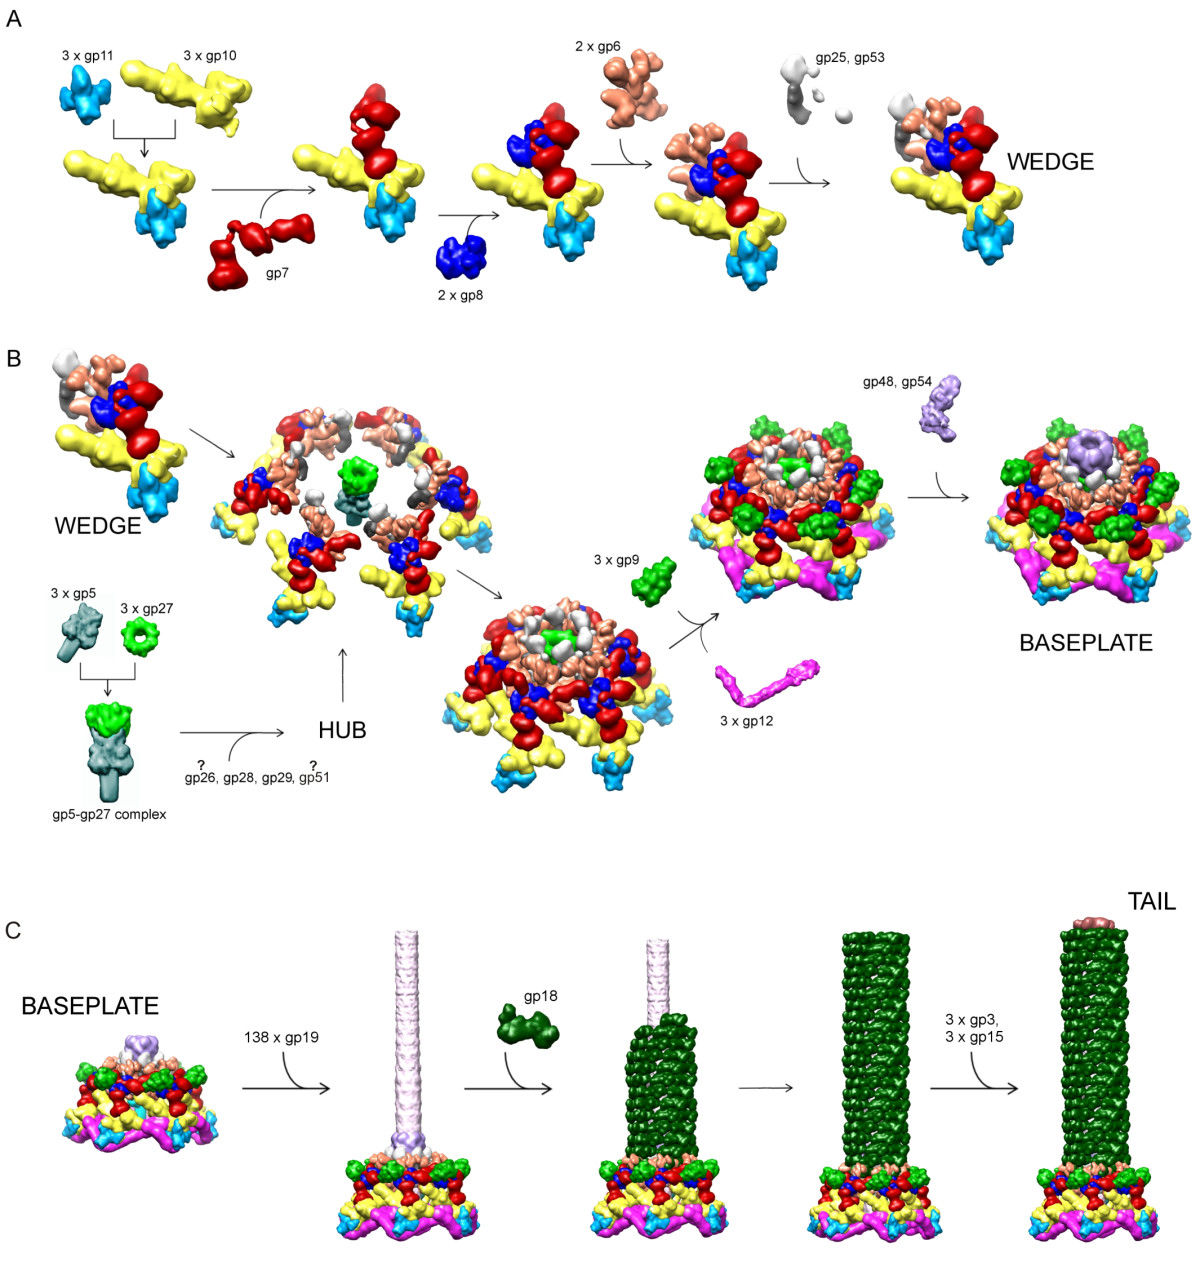
\includegraphics[width=\textwidth, trim={7 105 0 80}, clip]{/Users/joehealey/Documents/Warwick/PhD/Thesis/chapters/intro/img/t4assembly.jpg}
        \captionsetup{singlelinecheck=off, justification=centering, font=footnotesize, aboveskip=15pt, belowskip=10pt}
        \caption{}
        \label{baseplateformation}
    \end{subfigure}%
 
    \begin{subfigure}[h]{\textwidth}
        \centering
        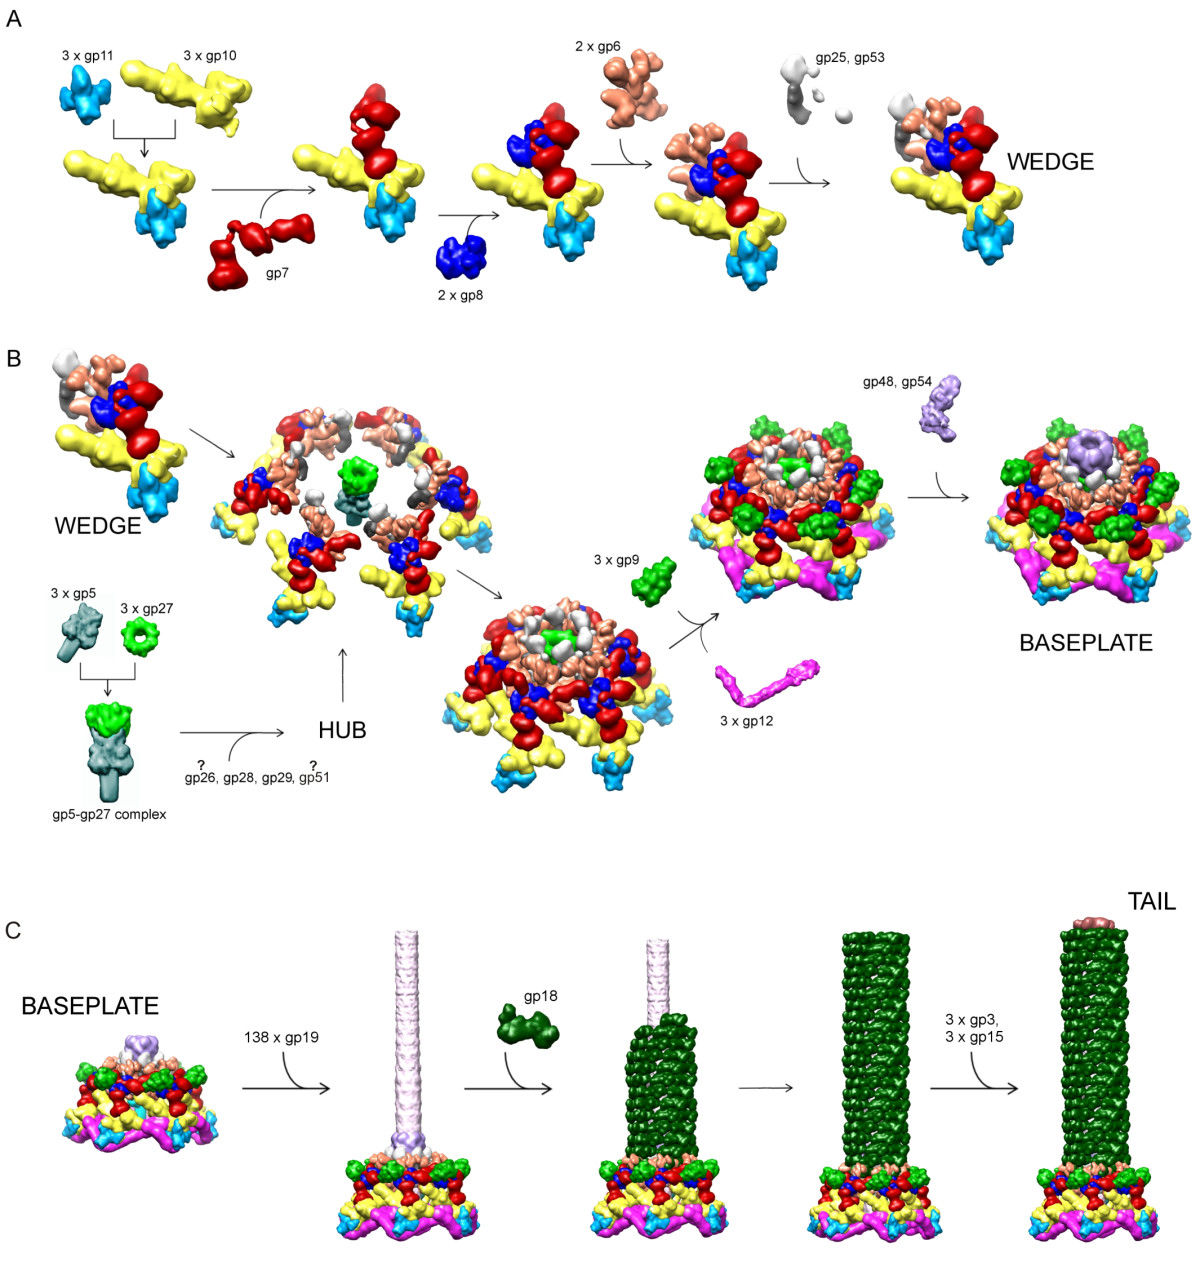
\includegraphics[width=\textwidth, trim={5.5 0 0 210}, clip]{/Users/joehealey/Documents/Warwick/PhD/Thesis/chapters/intro/img/t4assembly.jpg}
        \captionsetup{singlelinecheck=off, justification=centering, font=footnotesize, aboveskip=15pt, belowskip=10pt}
        \caption{}
        \label{tubeformation}
    \end{subfigure}%

	\captionsetup{singlelinecheck=off, justification=justified, font=footnotesize, aboveskip=10pt}
	\caption[Assembly of the T4 phage tube and baseplate]{\textsc{\normalsize The structural components of T4 and their stoichiometric assembly.} \vspace{0.1cm} \newline \textbf{(A)} The formation of the  ``baseplate wedge" subunit, which is, itself comprised of 6 different proteins and which makes up the majority of the baseplate. \textbf{(B)} Shows the formation of the complete baseplate, where the spike baseplate hub complex and tail fibres are added. The overall baseplate is made up of 6 wedge complexes which are further complexed together, with the addition of tail fibres and a number of other baseplate proteins including the collar. \textbf{(C)} A depiction of the complex between the baseplate structure and the polymerisation of the tail tube. The collar interfaces with the interior tube, around which almost 150 copies of gp18 are helically polymerised before termination and capping. Adapted and reproduced from \cite{Leiman2004} and \cite{Yap2014a}.}
	\label{t4assemblyflowchart}
\end{figure}
 %%%%%%%%%%%%%%%%%%%%%%%%%%%%%%

\begin{figure}[p]
\thisfloatpagestyle{augment}

\centering
\tabskip=0pt
\valign{#\cr
\hbox{%
    \begin{subfigure}[b]{0.45\textwidth}
        \centering
        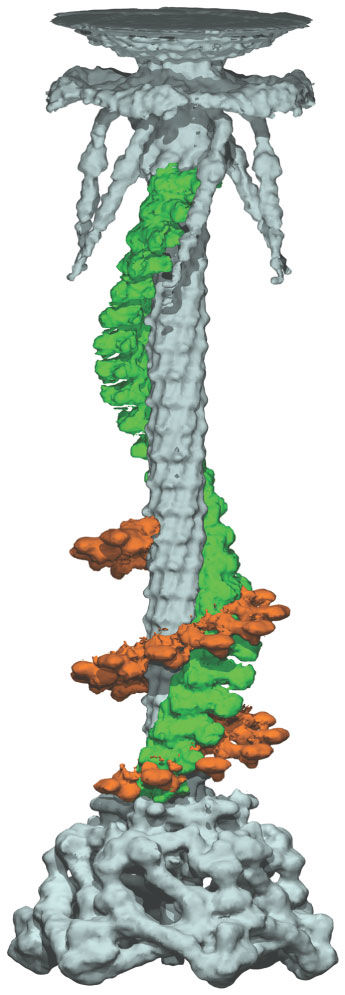
\includegraphics[width=\textwidth, trim={0 0 0 10}, clip]{/Users/joehealey/Documents/Warwick/PhD/Thesis/chapters/intro/img/nsmb975-F5.jpg}
        \captionsetup{singlelinecheck=off, justification=centering, font=footnotesize, aboveskip=10pt}
        \caption{}
        \label{t4sheaths}
    \end{subfigure}%
}\cr
\noalign{\hfill}
\hbox{%
    \begin{subfigure}[t]{0.45\textwidth}
        \centering
        \scalebox{-1}[1]{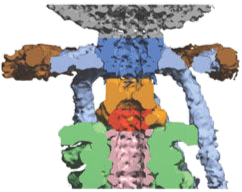
\includegraphics[width=\textwidth, trim={0 0 0 0}, clip]{/Users/joehealey/Documents/Warwick/PhD/Thesis/chapters/intro/img/nsmb975-F2.png}}
        \captionsetup{singlelinecheck=off, justification=centering, font=footnotesize, aboveskip=10pt}
        \caption{}
        \end{subfigure}%
}\vfill
  \hbox{%
    \begin{subfigure}[t]{0.42\textwidth}
        \centering
        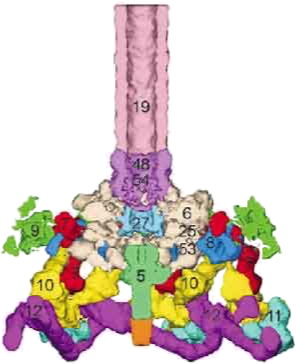
\includegraphics[width=\textwidth, trim={0 0 0 0 }, clip]{/Users/joehealey/Documents/Warwick/PhD/Thesis/chapters/intro/img/nsb970-F1.png}
        \captionsetup{singlelinecheck=off, justification=centering, font=footnotesize, aboveskip=10pt}
        \caption{}
    \end{subfigure}%
}\vfill
    \hbox{%
        \begin{subfigure}[t]{0.45\textwidth}
            \centering
            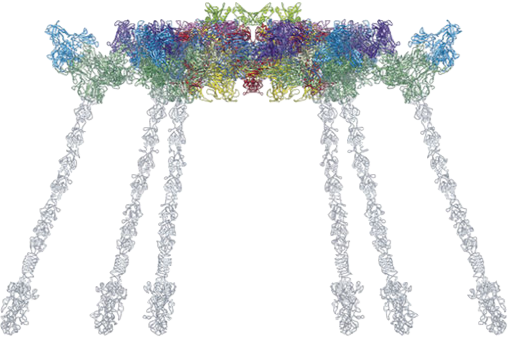
\includegraphics[width=\textwidth, trim={0 0 0 0}, clip]{/Users/joehealey/Documents/Warwick/PhD/Thesis/chapters/intro/img/nature17971-f1.png}
%            \begin{tikzpicture}
%            \node[inner sep=0] (image) {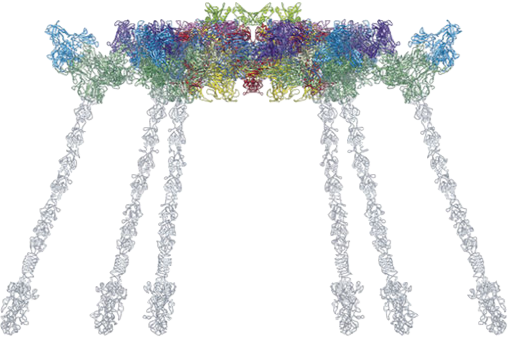
\includegraphics[width=\textwidth, trim={380 480 10 450}, clip]{/Users/joehealey/Documents/Warwick/PhD/Thesis/chapters/intro/img/nature17971-f1.jpg}};
%                    \begin{scope}[x={(image.south east)},y={(image.north west)}]
%                    \draw [fill=white] (10,1) -- (10,3) -- (10,4) -- cycle;
%            \end{scope}
%            \end{tikzpicture}
            \captionsetup{singlelinecheck=off, justification=centering, font=footnotesize, aboveskip=15pt}
            \caption{}
            \label{extendedtailfibres}
        \end{subfigure}%    
  }\cr
}
	\captionsetup{singlelinecheck=off, justification=justified, font=footnotesize, aboveskip=10pt}
	\caption[Resolved T4 Bacteriophage Structures from literature]{\textsc{\normalsize A selection of the resolved structural components of Bacteriophage T4.}\vspace{0.1cm} \newline \textbf{(A)} The T4 EM density reproduced from \cite{Kostyuchenko2005}, the helical outersheath protofilaments are shown in the extended (green) and contracted (orange) conformations. \textbf{(B)} The architecture of the `neck'/`collar' region of the T4 phage, showing the top of the tube. Adapted and  reproduced from Kostyuchenko \emph{et al.} also. \textbf{(C)} The intricate baseplate architecture (shown as a slice-through), adapted and reproduced from \cite{Kostyuchenko2003}. \textbf{(D)} The structure of the lower baseplate complex, showing the extended short tail fibres (they are `retracted' in \textbf{A} and \textbf{C}) adapted from \cite{Taylor2016}. The structure of the genome-containing capsid has been omitted, as the similarity to the tail and baseplate is more relevant. Augmented reality structures coloured according to cylinder radius (red ($\leq$100\AA) to blue ($\leq$20\AA). }
	\label{t4structure}
\end{figure}

\clearpage

\subsubsection{Of PVCs and R-type Pyocins/Tailocins}
The R-type pyocins, particularly those of \emph{Pseudomonas aeruginosa}, have been among the longest studied caudate structures, if Myophages such as those just discussed are discounted, with papers describing their structure and activity as far back as 1965 \citep{Ishii1965}, and they were discovered as early as 1954 \citep{jacob1954biosynthese}. Nevertheless, it took until 2015 for the structure of one of these tailocin structures to be resolved fully \citep{Ge2015} (see \vref{pyocinstructure}). A rapidly growing body of data on the specificity, activity and structure of these types of macromolecular complexes is appearing. `Tailocins' have attracted much attention recently due to their potential use as an alternative to phage therapy. The prospect of utilising bacteriophages has made the public and some of the scientific community understandably nervous, due to their uncontrolled, rapid replication within bacteria, and the introduction of foreign DNA in to the body's microbiome. Tailocins have alleviated some of these concerns due to their highly specific bactericidal activity, similar to phage, but without containing any nucleic material and thus no replicative capacity, and they appear tractable for engineering \citep{Scholl2008}.

Tailocins are so called as they are comprised of bacteriophage tail tube, baseplate and fibre structures, without a capsid or head \citep{Ishii1965}. Bacteria have co-opted these structures in to their genomes such that they can be used as highly specific antimicrobials against other, potentially closely related bacteria, providing considerably higher selective toxicity than is attainable through small molecule antimicrobials \citep{Heo2007}. This section specifically focuses on the ``R-Type" pyocins, which are considered a subclass of bacteriocins (protein or peptide toxic molecules effective against other bacteria; colicins are another well known example). They take their name from the fact that they are `Rod'-like phage tails, being demarcated from the F (`flexious') and S (soluble) type bacteriocins. They derive the name `pyocin' from their discovery in \emph{P. aeruginosa}, as mentioned, as it was renamed from \emph{Pseudomonas pyocynia}. The F-type pyocins are also phage tail like structures, but the tails are not straight tail rods, instead being somewhat curved, and crucially, they are noncontractile, meaning they are more closely related to P2 and $\lambda$ phages, than T-even \emph{Caudoviriales} \citep{Michel-Briand2002,Nakayama2000}. The S-type bacteriocins are small, soluble antimicrobials, more reminiscent of small molecule compounds, and cannot be sedimented or visualised by EM, unlike the F and R types \citep{Heo2007, kageyama1975bacteriocins}. As with the previous section on T4, \vref{pyocinems} shows a selection of R-type pyocin molecules as observed via EM. Hopefully the reader can already appreciate the similarities between the PVCs as shown in \vref{PVCems} and the pyocins in the figures below.


\vspace{0.2cm}
\begin{figure}[h]
\centering
    \begin{subfigure}[b]{0.4\textwidth}
        \centering
        {%
\setlength{\fboxsep}{0pt}%
\setlength{\fboxrule}{1pt}%
        \fbox{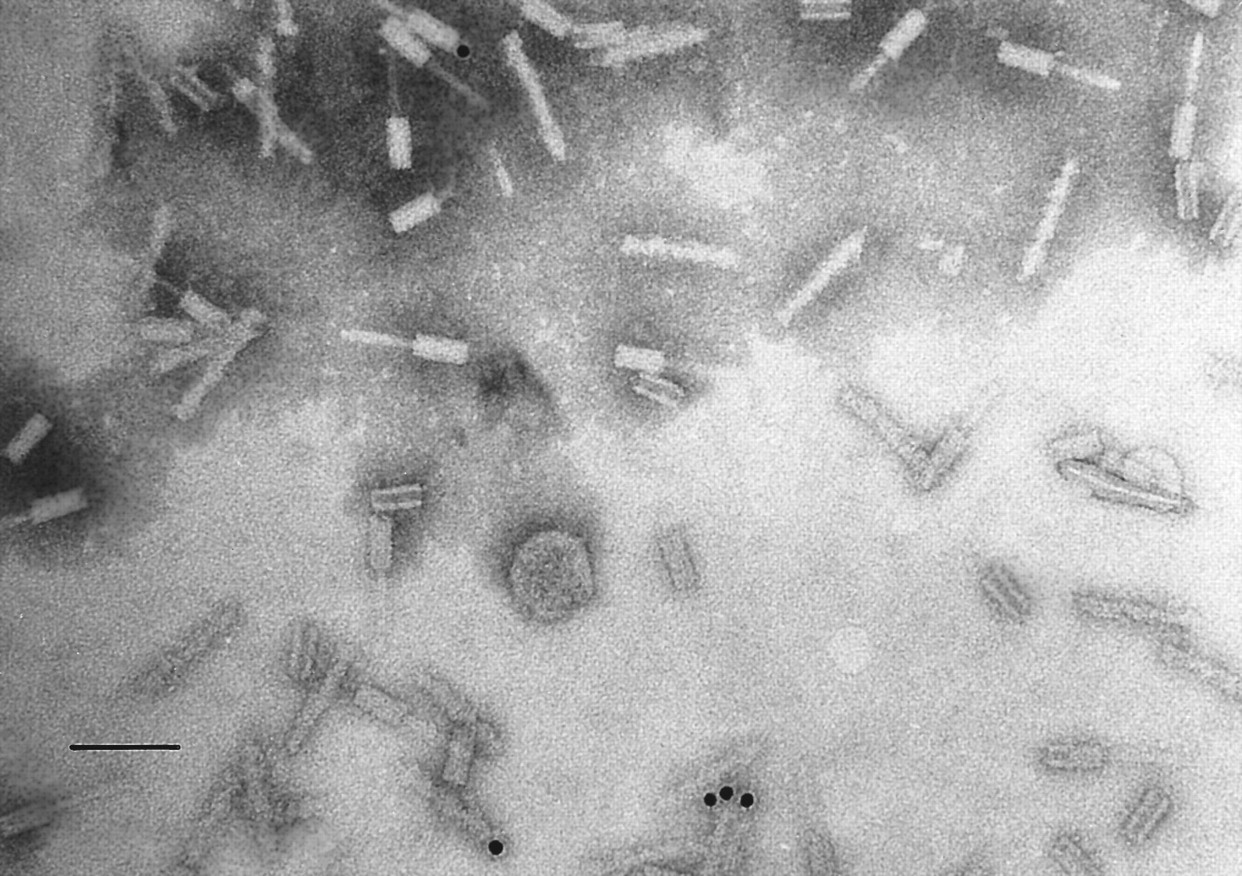
\includegraphics[width=\textwidth, trim={0 98 0 0}, clip]{/Users/joehealey/Documents/Warwick/PhD/Thesis/chapters/intro/img/pyocin.jpg}}
            }%
    \end{subfigure}%
        \begin{subfigure}[t]{0.18\textwidth}
        \centering
        {%
\setlength{\fboxsep}{0pt}%
\setlength{\fboxrule}{1pt}%
        \fbox{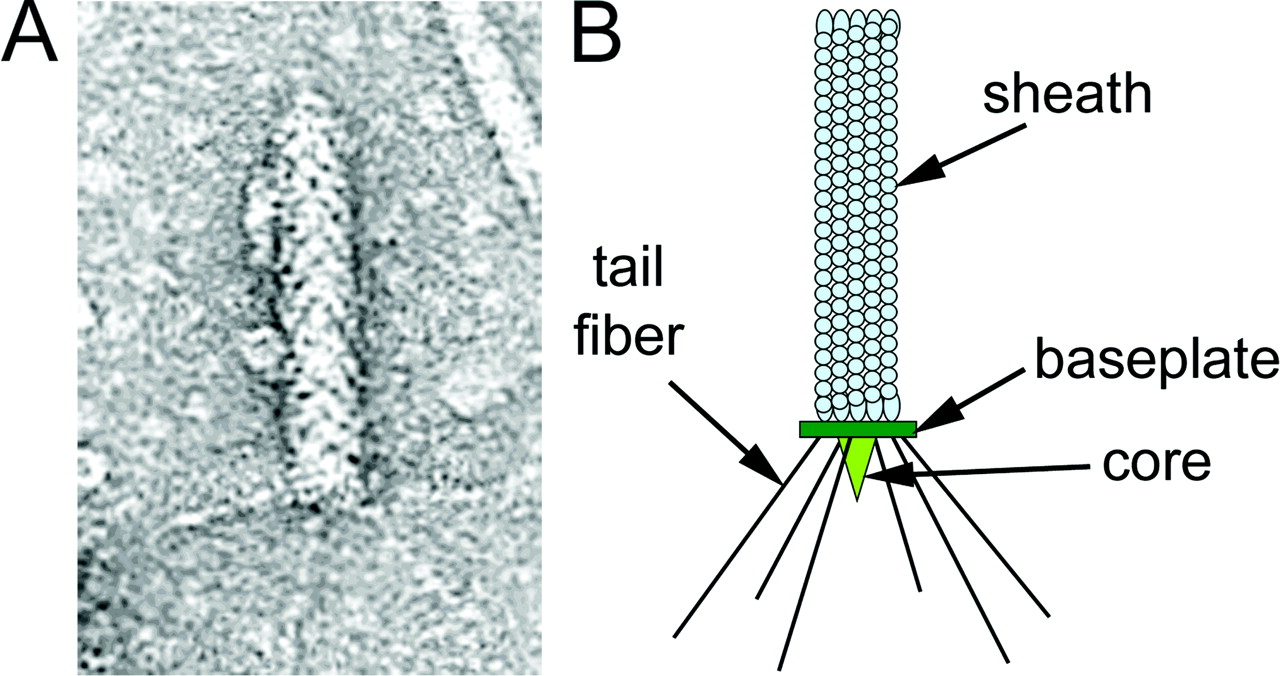
\includegraphics[width=\textwidth, trim={79 10 760 51}, clip]{/Users/joehealey/Documents/Warwick/PhD/Thesis/chapters/intro/img/afplarge.jpg}}
        }%
    \end{subfigure}%
    \begin{subfigure}[t]{0.4\textwidth}
        \centering
        {%
\setlength{\fboxsep}{0pt}%
\setlength{\fboxrule}{1pt}%
        \fbox{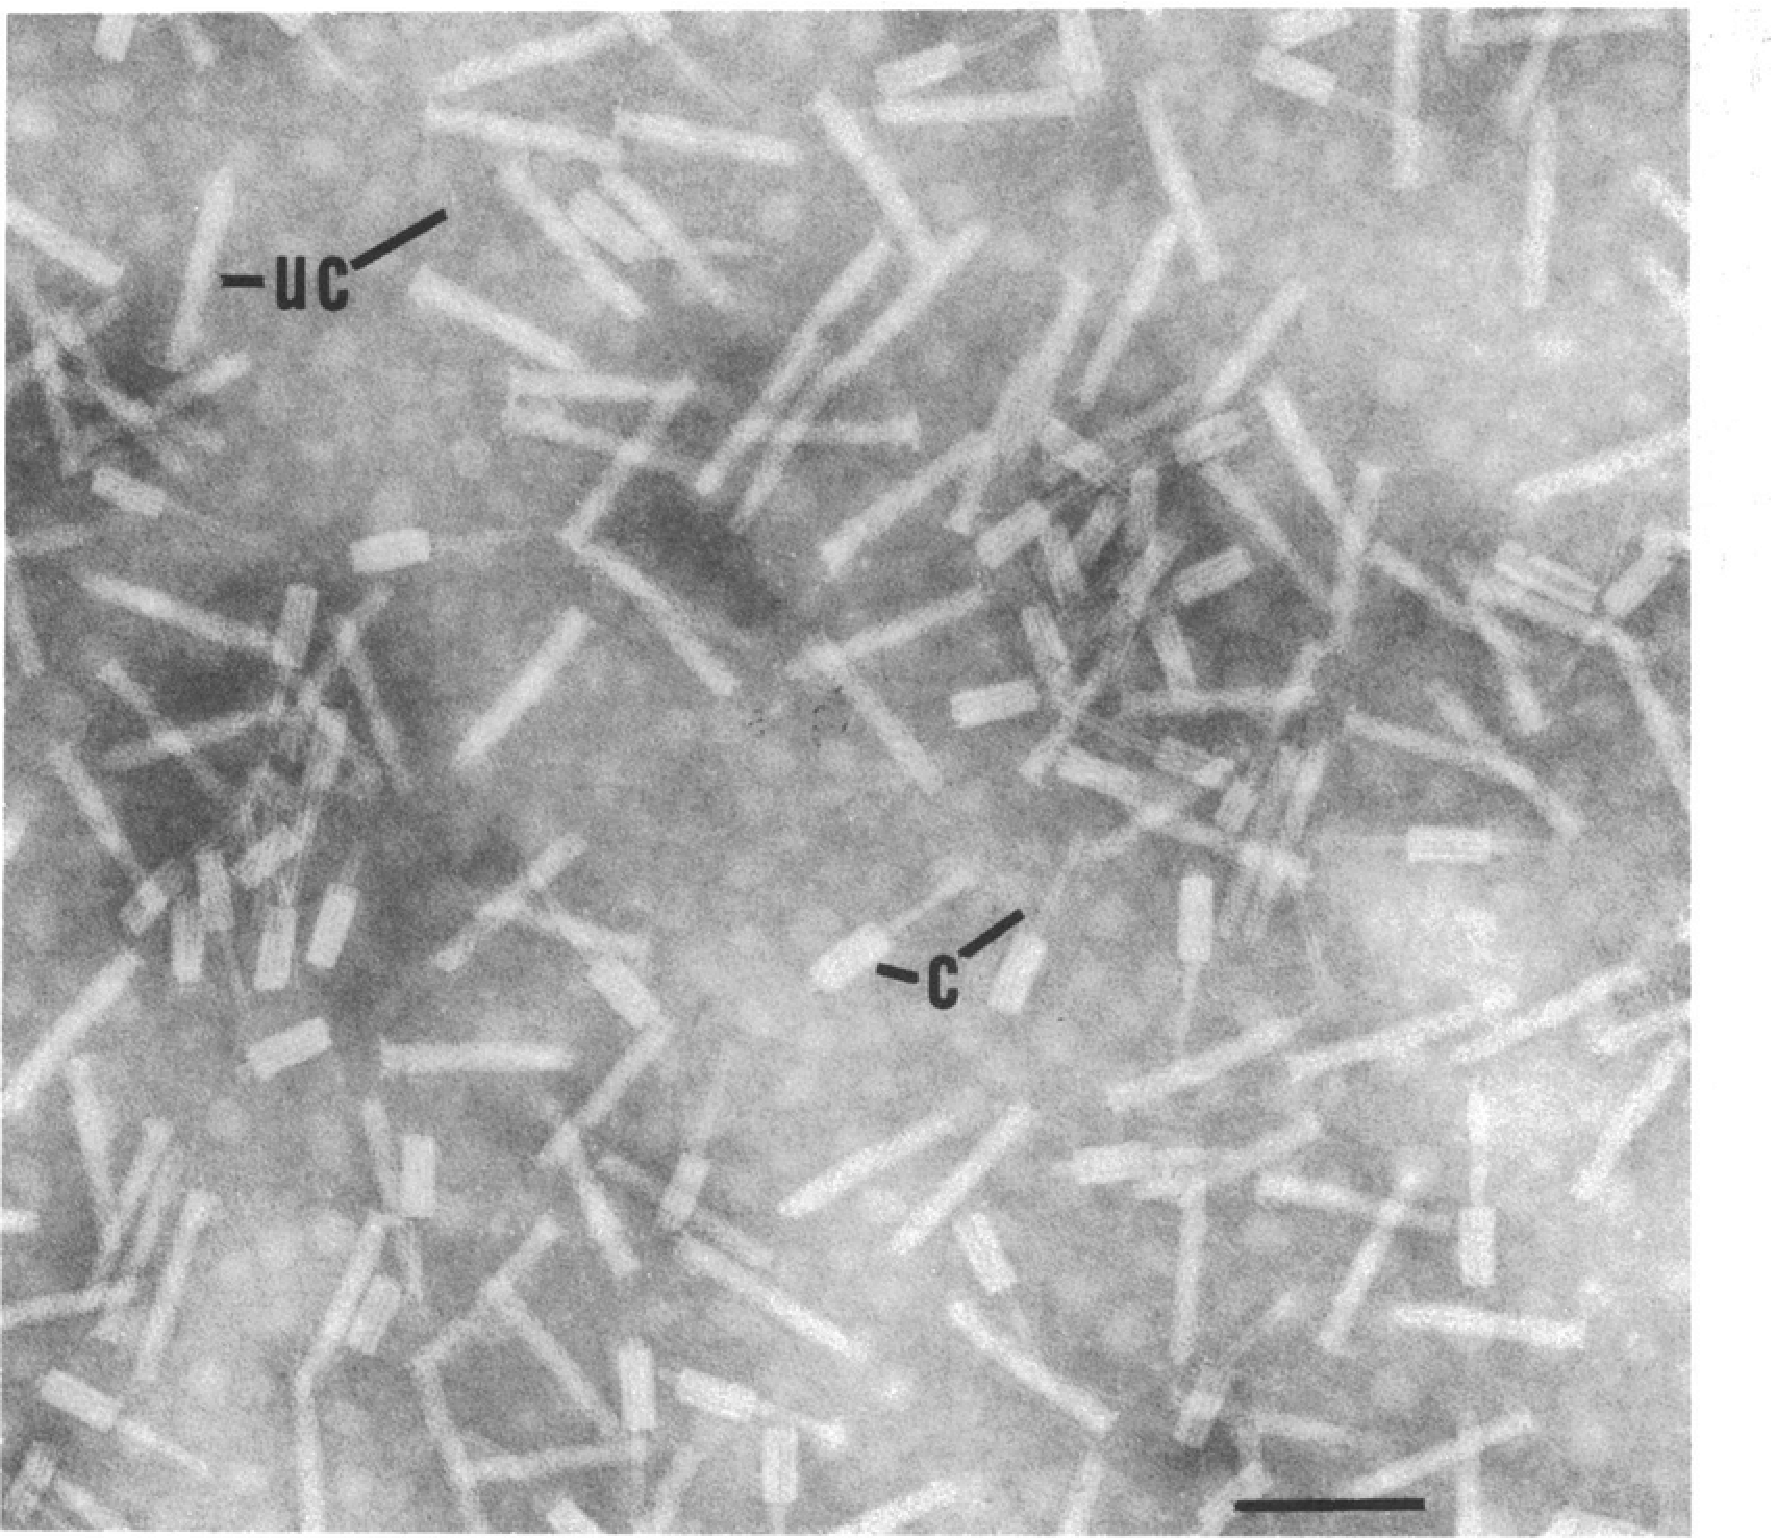
\includegraphics[width=\textwidth, trim={5 200 60 46}, clip]{/Users/joehealey/Documents/Warwick/PhD/Thesis/chapters/intro/img/em_labelled.pdf}}
        }%
        \end{subfigure}%
	\captionsetup{singlelinecheck=off, justification=justified, font=footnotesize, aboveskip=10pt}
	\caption[Electron micrographs of \emph{Pseudomonas} R-type pyocins]{\textsc{\normalsize Electron Micrographs of \emph{Pseudomonas} R-type pyocin particles}\vspace{0.1cm} \newline The left panel shows a number of R-type pyocin molecules purified. The contracted nature of several of the particles reveals clearly the size difference between the inner and outer sheaths. Reproduced from \cite{Lee1999}. The central panel shows a close up image of an individual pyocin particle, where the caudate structure and presence of at least 4 tail fibres is apparent (reproduced from \cite{Williams2008a}. The right hand panel shows R-type pyocin particles in a semi-purified form. The annotations on the image from the original document denote \textbf{UC} - uncontracted particles, and \textbf{C} - contracted particles. Reproduced from \cite{Morse1976}.}
	\label{pyocinems}
\end{figure}


R-type pyocins exert their antimicrobial activity in a similar fashion to bacteriophages, by first using their tail fibre proteins to bind with the lipopolysaccharides (LPS) of other Gram negative bacterial cells of closely related strains. The binding occurs strongly, which provides the necessary anchorage for the next step of toxicity - puncturing. The contractile system, as in the Myophages, drills the tail tube and spike in to the surface of the cell, creating a pore. Unlike the Myophages however, the pyocins contain no translocated material (DNA nor protein) and instead, simply cause a rapid and lethal depolarisation of the bacterial membrane \citep{Uratani1984}. The consensus, at least, is that no material is translocated, though some papers have shown single stranded nucleotide cargoes \citep{Lee1999} - this may be an exception, rather than the rule though. Such is the efficacy and potency of this mechanism of killing, that the pyocins demonstrate `single hit kinetics', meaning a single pyocin complex is sufficient to kill an individual cell \citep{OHKAWA1973}. Roughly 100-200 pyocins can be produced from a single host bacterium, with the first active complexes matured after as little as 45 minutes after induction \citep{Michel-Briand2002, Shinomiya1972, Scholl2008}.

The R-type pyocins structurally resemble something of a `halfway house' between phage and PVC-like systems; they have `streamlined' genetics, by way of removal of the capsid genes and the associated replicative machinery, though the evolutionary relationships between them remain unknown. The pyocins are also a good example of the ubiquity of contractile tail systems in nature, underscoring their potentially pivotal role in the shaping of ecosystems, being elaborated by around 90\% of \emph{Pseudomonas} strains \citep{Michel-Briand2002}, being widespread amongst Gram negatives (particularly among other \emph{Enterobacteriaceae}) \citep{Coetzee1968} and examples also being found in Gram positives such as \emph{Listeria} \citep{Zink1995} and \emph{Staphylococcus} \citep{Birmingham1981, Scholl2008}. 

Even with this seeming ubiquity among various clades within bacteria, it's interesting to observe and speculate at this point, on the possible link between these microbial `weapons' and their abundance in species of bacteria which are thought to have some marine origins. \emph{Pseudomonas} is known to be associated with marine and generally aquatic environments, and this has been a long running hypothesis for the origins of \emph{Photorhabdus} itself (two `smoking guns' for this being that it has retained the \emph{lux} operon, which is otherwise exclusive to marine organisms, and its frequent isolation near coastlines). It seems that the ability to produce a caudate structure which can be deployed at a distance could have some extra utility in aquatic environments - and some further examples of innovative tailocin like structures are discussed in Section 1.2.3.5.1 on page 47 and Section 1.2.3.5.1 on page 48. \cite{Persson2009} have also made a similar observation, when they studied the prevalence of various pathogenicity islands in marine organisms from the Global Ocean Sampling dataset, including islands like the Antifeeding prophage (see \vref{afp}).

The seminal paper which finally resolved the intricacies of the the structure of the R-type pyocins was that of \cite{Ge2015}. Not only were they able to obtain high resolution EM maps of the structure, they managed to resolve, atomistically, both the pre- and post-contraction states. \vref{pyocinstructure} reproduces this data.


\begin{figure}[p]
\thisfloatpagestyle{augment}
\centering
\tabskip=0pt
\valign{#\cr
\hbox{%
    \begin{subfigure}[b]{0.3\textwidth}
        \centering
        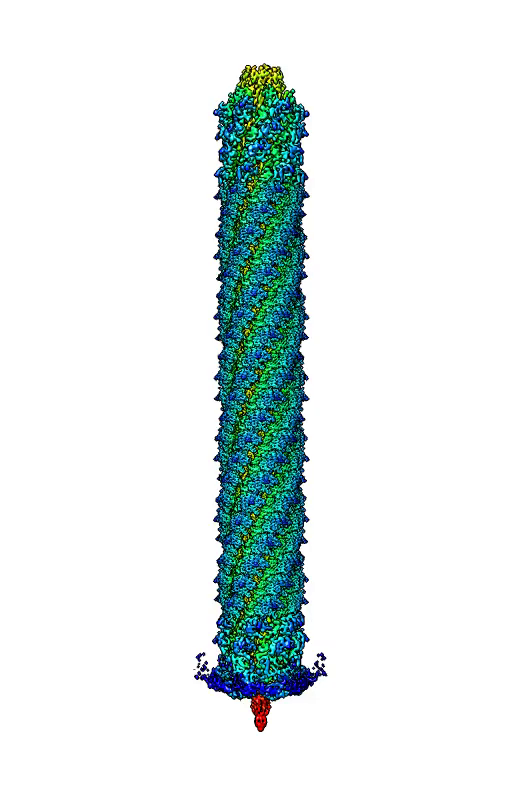
\includegraphics[width=\textwidth, trim={170 40 180 60}, clip]{/Users/joehealey/Documents/Warwick/PhD/Thesis/chapters/intro/img/videostill.png}
        \captionsetup{singlelinecheck=off, justification=centering, font=footnotesize, aboveskip=10pt}
        \caption{}
        \label{videostill}
    \end{subfigure}%
}\cr
\noalign{\hfill}%\vspace{1cm}
\hbox{%
    \begin{subfigure}[t]{0.65\textwidth}
        \centering
        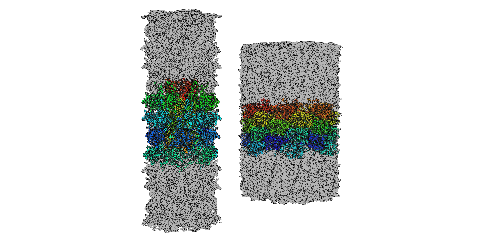
\includegraphics[width=\textwidth, trim={65 2 65 2}, clip]{/Users/joehealey/Documents/Warwick/PhD/Thesis/chapters/intro/img/pyocin_maps.pdf}
        \captionsetup{singlelinecheck=off, justification=centering, font=footnotesize, aboveskip=10pt}
        \caption{}
        \end{subfigure}%
}\vfill
    \hbox{%
        \begin{subfigure}[t]{0.68\textwidth}
            \centering
            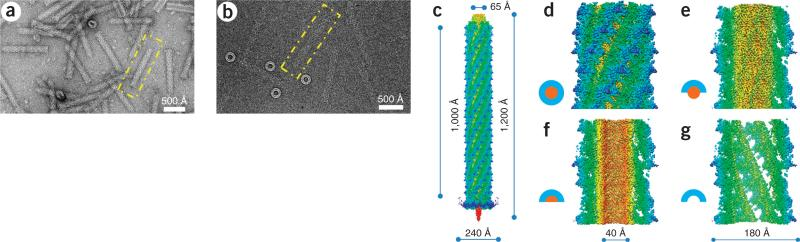
\includegraphics[width=\textwidth, trim={200 0 0 0}, clip]{/Users/joehealey/Documents/Warwick/PhD/Thesis/chapters/intro/img/pyocintube.jpg}
            \put(-91,168){\obscure{0.5cm}{0.5cm}}
            \put(-91,76){\obscure{0.5cm}{0.5cm}}
            \put(-195,168){\obscure{0.5cm}{0.5cm}}
            \put(-195,77){\obscure{0.5cm}{0.5cm}}
            \put(-279,167){\obscure{0.5cm}{0.5cm}}
            \captionsetup{singlelinecheck=off, justification=centering, font=footnotesize, aboveskip=15pt}
            \caption{}
            \label{slicedtube}
        \end{subfigure}%    
  }\cr
}
	\captionsetup{singlelinecheck=off, justification=justified, font=footnotesize, aboveskip=10pt}
	\caption[Resolved R-type Pyocin Structures from \cite{Ge2015}]{\textsc{\normalsize The structures of the R-type pyocin from \cite{Ge2015}.}\vspace{0.1cm} \newline \textbf{(A)} The reconstructed pyocin EM density reproduced from the Supplementary Video 1 of the \cite{Ge2015} paper as a snapshot. The structure is coloured according to its distance from the central axis (colder colours are further away from the centre). \textbf{(B)} Shows the extended and contracted sheath structures for the pyocin from EMDB-6270 (extended) and EMDB-6271 (contracted) with the fitted PDBs 3J9Q and 3J9R respectively. These figures were made using the published data, but reproduced independently using UCSF Chimera \citep{Pettersen2004}. \textbf{(C)} Shows sequential cut-aways of the sheaths with \AA{}ngstrom measurements of the inner and outer diameters and lengths. The coloured circles adjacent to each sub-panel are a key to which tube faces have been sliced through (orange = inner, blue = outer).}
	\label{pyocinstructure}
\end{figure}

\clearpage


From \vref{pyocinstructure} the helical nature of the outer sheath is quite apparent. Interestingly though, unlike the T4 phage structure, the inner sheath is not helically offset, instead being a direct stack of hexamers forming the equivalent of the gp19 toroids. The outer sheaths are helically offset relative to one another by 18.3$^{\circ}$, with a right handed spiral, and are translated by 38.4$^{\circ}$ along the vertical helix axis \citep{Ge2015, Kube2015a}. Thus the hexameric helix is, in effect, more `tightly wound', by having a greater deal of twist, and less vertical rise per unit versus the T4 sheath (in the extended configuration). The outer sheath differs further still as it is comprised of much simpler monomers. The molecular weight of the gp18 monomers is $\approx$ 71.3 kDa, whereas the equivalent outer sheath protein in the R-type pyocin is only 41.2 kDa. This can also be seen from the structures themselves, as the pyocin monomers seem to lack the protrusions that the T4 gp18 protomers have to quite the same degree, though there is still a noticeable ridge-trough-ridge architecture to the tube \citep{Kube2015a}. From the atomic reconstruction, it was shown by Ge and colleagues that each protomer of the outer sheath interacts with the adjacent 2 protomers via extensions of the N and C termini of the individual monomers with the C-terminal reaching out to the monomer to the right, and the N-terminal to the left. Thus the outer sheath of the R-type pyocin actually more closely resembles a mesh, like a chain-link fence, encompassing the inner sheath, but with the ability to transduce a contraction force along its length \citep{Ge2015}. The bottom left panel of \vref{slicedtube} demonstrates this, as the outer sheath cutaway can be seen through completely from the interior. This interaction has also been observed in bacterial pili and Type 6 Secretion Systems, and previously referred to as the ``$\beta$-augmentation mechanism" \citep{Remaut2006}. Mutagenesis studies showed that these interwoven strands were essential for the contractile mechanism in the T6SS, though were not required for assembly, suggesting that hydrostatics are largely responsible (which is also consistent with the spontaneous self assembly of Hcp monomers seen in \cite{Ballister2008}) \citep{Kudryashev2015, Clemens2015}. The Ge et al. paper also made the observation that there is no structural interaction between subunits of the outer sheath beyond the terminal extensions. The primary interactions in the outer sheath are actually along individual helical protofilaments - i.e. one subunit interacts with the subunits above-right, and below-left of it. 

The inner sheaths rings display complementary surface charge, further suggesting that they are self-assembled in a hydrostatically driven manner. In effect, each disk could be considered a bar magnet, with an electrostatic `north and south pole' (really an electrostatic dipole), ensuring they assemble correctly in a head-to-tail fashion \citep{Ge2015}. The inner sheath monomers of the pyocin consists of 2 anti-parallel $\beta$-sheets, which are orthogonal to one another in strand direction by approximately 90$^{\circ}$. It was noted that they form a similar structure to the well known `jelly roll' or `cupin' fold where 2 sets of 4 $\beta$-strands are opposed to one another \citep{Richardson1981, Dunwell2004}, but are actually thought to be unrelated, despite this domain being highly conserved in other viral and (to a lesser degree) cellular protein sequences. The 6 monomers combine to form one of the largest $\beta$-barrel structures to be resolved yet with 24 $\beta$-strands forming the inner circumference of the lumen \citep{Ge2015}.

Ge and colleagues have recapitulated an often seen homology modelling approach for the core lumen of the pyocin, and compared its surface charge, and smooth bore to the orthologues from phage $\lambda$ \citep{Pell2009a}, the T6SS \citep{Jobichen2010}, and phage PS1. They observed that the inner lumen of the R-type pyocins are primarily negatively charged, consistent with its putative role in depolarisation of cells by de-protonating the cell interior. Conversely, the inner sheaths of phage are typically positively charged to assist in the conveyance of negatively charged DNA. As the electrostatic potential of proteins is, of course, extremely variable, according to the amino acid sequence and manner of tertiary fold, the Hcp monomers which comprise the T6SS inner sheath have been shown to be largely neutral overall. This then enables these systems to convey all manner of protein cargoes, without any `selectivity'. \vref{structbioinfo} replicates this process in the context of the PVCs sheath proteins, to take a first look, albeit \emph{in silico} at this stage, at the sheath structures and any potential relation to their cargo.

The inner and outer sheaths interact primarily electrostatically, with a small triangular region of negative charge on the outer sheath (on 2 `attachment' helices that protrude upward) corresponding to a triangular region of positive charge on the inner sheath. This causes the inner sheath that corresponds to a given tier/disk in the outer sheath to be offset upwards by roughly 15 \AA, and thus an outer sheath monomer straddles 2 inner tiers. Ge and colleagues showed that this reversible electrostatic interaction is important, as the outer sheath increases in diameter upon contraction, and detaches itself from the inner sheath, enabling it to protrude beyond the end of the outer sheath in order to execute its function and traverse the membrane of a target cell.

All that remains of the structure, the spike complex, baseplate, and tail fibres, were not well resolved in the Ge et al. study unfortunately. They obtain reasonable densities for the proximal baseplate, being able to identify `spokes' which connect it to the spike, but do not speculate on, nor provide, further detail or its atomistic structure. It is evident from \vref{videostill}, however, that the baseplate is much stripped down versus the T4, mirroring the streamlining that is also seen in the removal of the capsid, long fibres, and replicative machinery, serving purely as a mounting point for the tail fibres seemingly. As with the baseplate, for the spike complex, detail was lost as a result of their averaging process. Fortunately, its density is also easy to identify from \vref{videostill}, and Ge et al report that they were able to locate a co-ordinated metal ion in the tip (typically iron or zinc), which is a hallmark of gp5-gp27 and VgrG-like spike proteins \citep{Shneider2013, Kube2015a, Browning2012}.

In summary, the structure of the R-type pyocins appears to more accurately reflect the simplicity that is seen in the PVC operons, following a streamlining process associated with non-replicative entities. From the studies to date however, pyocins have only ever demonstrated anti-prokaryotic activity, while on the other hand, PVCs have only ever demonstrated anti-eukaryotic activity. Now, while this may be due to not testing each complex against an exhaustive repertoire of prokaryotes and eukaryotic cell types, these specificities seem to fit with what is known of their basic biology. This means that there is still much to be discovered about what makes PVCs different, and allows them to act on various higher order cell types in the few genes that are remaining without fully understood functions.



\subsubsection{Of PVCs and the \emph{Serratia entomophila} ``Antifeeding prophage"}\label{afp}
This brings us to possibly the nearest cousins of the PVCs - the so-called ``Antifeeding Prophages" of \emph{Serratia}. The Afp was, until the advent of the \cite{Ge2015} paper, the best characterised, closest relative, of the PVCs, and much of what was hypothesised about them was based on analogous experiments on the Afps, borne on a plasmid of \emph{Serratia entomophila} \citep{Rybakova1994}. As its name suggests, like \emph{Photorhabdus}, \emph{S. entomophila} is another common insect pathogen, and they have been shown to be quite closely related \citep{Duchaud2003, Sproer1999, Brillard2002b}. \emph{S. entomophila} causes ``Amber Disease" in the New Zealand grass grub \emph{Costelytra giveni} (formerly \emph{Costelytra zealandica} \citep{Coca-Abia2016}) specifically, and has been used for some time now as a biopesticide \citep{Chattopadhyay2012, OpenderKoul2011}. Electron microscopy studies of purified particles revealed similar morphologies to the Pyocins and PVCs:


\vspace{0.1cm}
\begin{figure}[h]
\centering
    \begin{subfigure}[b]{0.41\textwidth}
        \centering
        {%
\setlength{\fboxsep}{0pt}%
\setlength{\fboxrule}{1pt}%
        \fbox{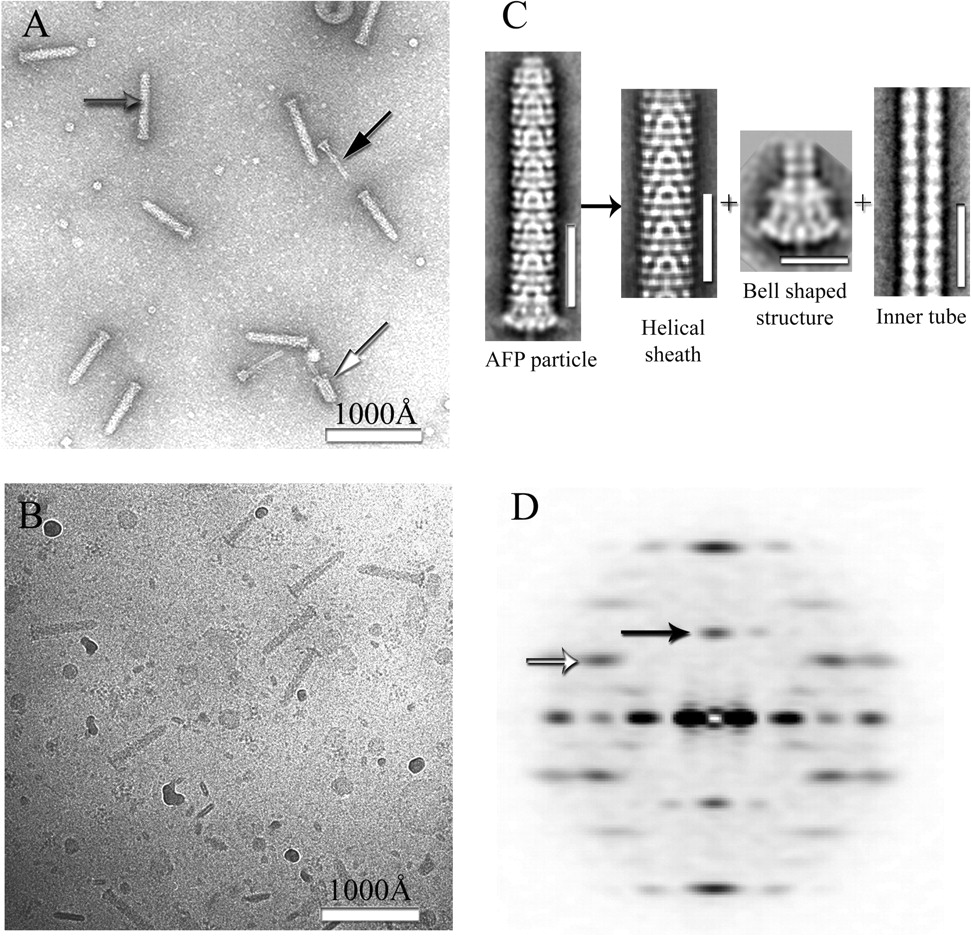
\includegraphics[width=\textwidth, trim={50 700 540 50}, clip]{/Users/joehealey/Documents/Warwick/PhD/Thesis/chapters/intro/img/afp_large.jpg}}
            }%
    \end{subfigure}%
        \begin{subfigure}[t]{0.16\textwidth}
        \centering
        {%
\setlength{\fboxsep}{0pt}%
\setlength{\fboxrule}{1pt}%
        \fbox{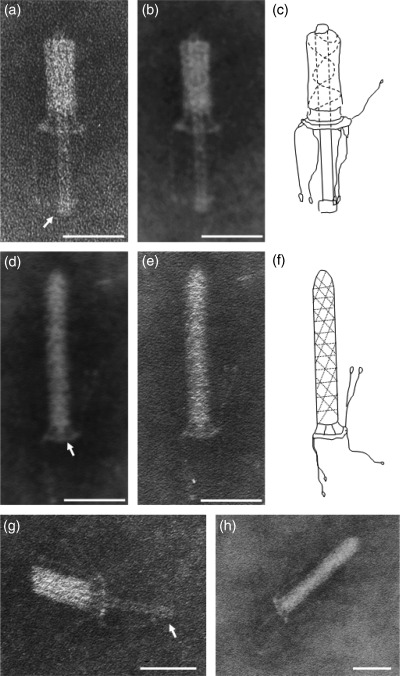
\includegraphics[width=\textwidth, trim={250 5 25 515}, clip]{/Users/joehealey/Documents/Warwick/PhD/Thesis/chapters/intro/img/Afpvariants.png}}
        }%
    \end{subfigure}%
    \begin{subfigure}[t]{0.41\textwidth}
        \centering
        {%
\setlength{\fboxsep}{0pt}%
\setlength{\fboxrule}{1pt}%
        \fbox{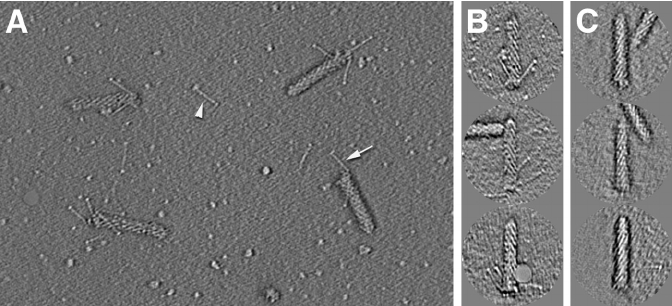
\includegraphics[width=\textwidth, trim={0 45 220 40.2}, clip]{/Users/joehealey/Documents/Warwick/PhD/Thesis/chapters/intro/img/Afp_tomogram.png}}
        }%
        \end{subfigure}%
	\captionsetup{singlelinecheck=off, justification=justified, font=footnotesize, aboveskip=10pt}
	\caption[Electron micrographs of the Antifeeding Prophage]{\textsc{\normalsize Electron Micrographs of the Antifeeding Prophage of \emph{S. entomophila}.}\vspace{0.1cm} \newline The left panel shows EMs of the Afps, revealing their ``bullet like" shape, and similarity to PVCs. The grey arrow denotes a mature, fully intact Afp particle. The black arrow highlights a ``Tube-Baseplate Complex". Adapted and reproduced from \cite{Sen2010}. The centre panel shows a close up of an individual mature Afp, it is just possible to make out the skirt-like formation of the baseplate, and a couple of tail fibres, including one pronate against the tube. Adapted and reproduced from \cite{Hurst2007}. The right hand panel shows more intact Afp particles, and particularly reveals the tail fibre like structures, of which multiple can be seen on any one particle, and some can even be seen loose on the grid (white arrows). Adapted and reproduced from \cite{Heymann2013}.}
	\label{afpEMs}
\end{figure}




The Afps were discovered on the 153,404 bp pADAP (``Amber Disease Associated Plasmid") plasmid \citep{Hurst2011a} due to their pathological effect against \emph{C. giveni}. The plasmid has been shown to contain other virulence factors such as the \emph{sep} toxins (homologues of the well characterised \emph{Photorhabdus} ``Toxin Complex" genes, and thought to be similarly mobile \citep{Dodd2006a}), which are the aetiological agents of ``Amber disease" (and of which \emph{Photorhabdus} also has analogues - in fact, one such \emph{sepC} analogue is a cognate PVC effector) \citep{Hurst2000}. It was observed in the \emph{sep} studies that another large locus on the plasmid caused a cessation of feeding effect 1 to 3 days after ingestion. In later efforts, this was identified as the ``Antifeeding prophage", and hence it earned its name \citep{Hurst2004}. Over almost 10 years, 4 primary papers were published which steadily elucidated the genetic components and pathology \citep{Hurst2004}, the regulation \citep{Hurst2007a} and the structural basis of Afp complexes \citep{Sen2010, Heymann2013}. Additionally, a number of papers were able to identify putative biological roles for some of the more enigmatic proteins in the locus \cite{Rybakova2013, Rybakova2015}. The presence of the Afp on the pADAP replicon was fortunate, as it allowed the whole operon to be subcloned in to lab \emph{E. coli} replicons with relative ease \citep{Hurst2004}. This has allowed quite extensive deletion/mutation studies to be conducted, as well as providing the material for structural resolution. To date, no PVC equivalents have been identified on plasmids in \emph{Photorhabdus}, though in \Plum{} TT01, 4 PVCs appear tandem to one another, surrounded by conjugation machinery and partitioning proteins such as \emph{mukB}, which may be suggestive of an ancestral recombination event between a large plasmid and the chromosome \citep{Yang2006}. More recently, another orthologue of the Afp, termed AfpX has been found in a further strain of \emph{Serratia}, \emph{S. proteamaculans}, once again located on a plasmid, is distinct from the `original' Afp in a number of ways which will be discussed in upcoming sections \citep{Hurst2018}.

The Afp operon is comprised of 18 proteins, termed Afp1-18. Analogues to sheath proteins, spike complexes, baseplate proteins and tail fibre proteins were able to be identified bioinformatically upon first sequencing. A number of proteins were matched to \emph{Photorhabdus} orthologues with unknown functions, revealing the close relationship between these 2 loci, though much of the operon remained poorly understood. Efforts by Rybakova and colleagues were able to shed some light on the roles of Afp14 and Afp16 in the control of tail assembly. In 2013, the function of Afp16 was determined to play a role in the tail length termination process, and stabilised the growing tail tube \citep{Rybakova2013}. Full deletion of this protein resulted in aberrant forms of the Afp, with variable lengths, as well as formation of so-called ``Tube-Baseplate complexes" (TBCs), which lacked much of the outer sheath, but were able to form a truncated inner sheath and seemingly full baseplate arrangement. Trans-expression of Afp16 did not restore a fully matured morphology to the Afps, suggesting that the expression patterns within the operon itself are also key to the self-assembly process, though exogenously applied purified Afp16 to pseudo-denatured Afps did exhibit some restored assembly - though again, not full length. Truncations of the C-terminus of the protein resulted in an intermediate morphology between the TBCs and a fully matured particle. It is still unclear at present how these proteins interact in order to produce the `finished product' however.

In 2015, Rybakova and colleagues were further able to elucidate the role of another enigmatic protein in the formation of the tail tube, this time identifying an analogue of a putative tape measure protein. Truncations of the protein resulted in concomitant shortenings of the elaborated Afp particles, and similarly, elongations of the sequence resulted in particles of increased tail length. Remarkably, there is a near exact linear relationship (R$^2$ = 0.92) between the length of known tail tubes and their associated tape measure proteins \citep{Rybakova2015, Pedulla2003}. Tape measure proteins are difficult to detect via homology alone, as their sequence appears to not be particularly restrictive to function, with no obvious conservation of known phage tape measure domains. The only real hallmarks that have been identified between varied orthologues are a relatively conserved distribution of hydrophobic residues, and atypically high degrees of alpha helical secondary structure. Unusually, the AfpX identified in \emph{S. proteamaculans} has 2 paralogues of the tape measure protein, which vary in length by 36 amino acids. Accordingly, when particles where identified micrographically, a wider distribution of sizes was observed than in the original Afp. The significance of this is not yet understood.

As with the PVCs, at least one of the genes at the 3'-most end of the operon (Afps 17 and 18) are predicted to encode toxic effectors, though unlike the PVCs, there do no not appear to be many variant forms. This is probably one of the reasons that \emph{S. entomophila} maintains a very specific pathogenicity against the grass grub. The Afps, by virtue of their toxic cargoes have been shown to have an LD$_{50}$ of as little as 500 individual Afp particles (though with the potential for multiple toxins to be present per Afp), against an entire insect \citep{Rybakova1994}.
{
\begin{figure}[p]
\thisfloatpagestyle{augment}
\centering
\tabskip=0pt
\valign{#\cr
\hbox{%
    \begin{subfigure}[t]{0.41\textwidth}
        \centering
        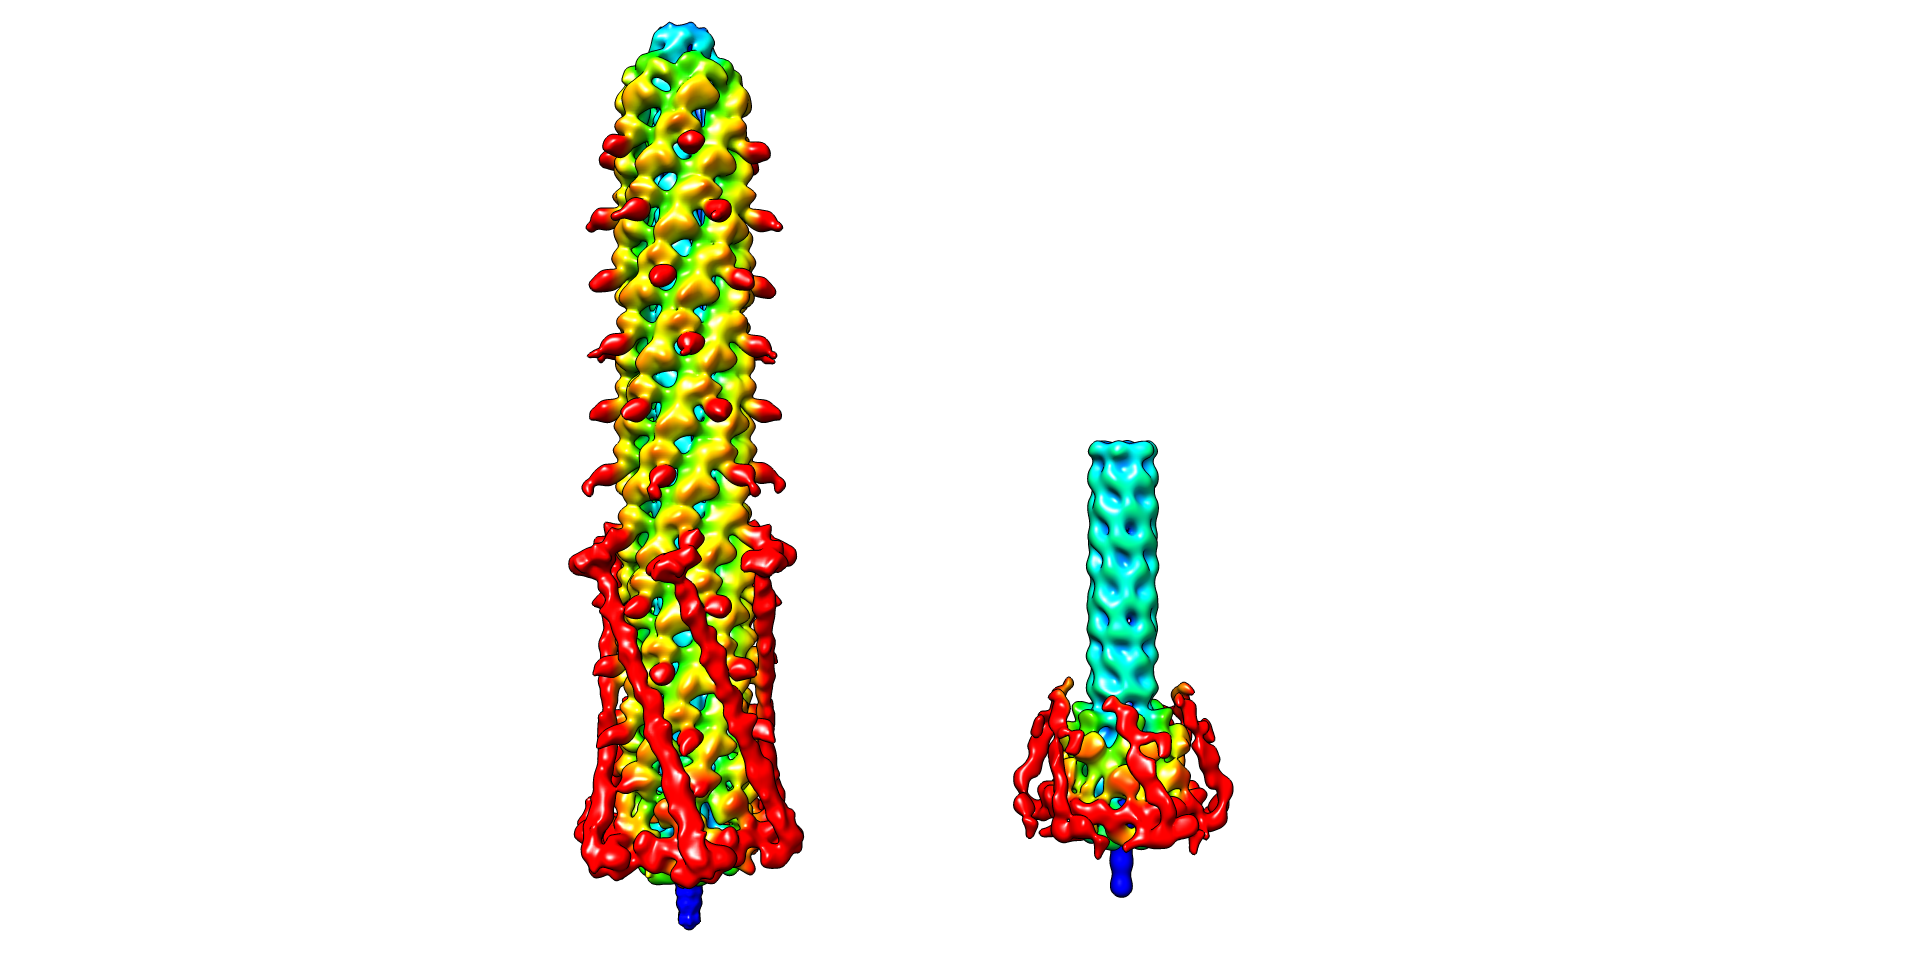
\includegraphics[width=\textwidth, trim={65 3 130 2}, clip]{/Users/joehealey/Documents/Warwick/PhD/Thesis/chapters/intro/img/afp_map_reconstructed.png}
        \captionsetup{singlelinecheck=off, justification=centering, font=footnotesize, aboveskip=10pt}
        \caption{}
        \label{afp1}
    \end{subfigure}%
}\cr
\noalign{\hfill}%\vspace{1cm}
\hbox{%
    \begin{subfigure}{0.58\textwidth}
        \centering
          \begin{tabular}{lr}
            \raisebox{-.5\height}{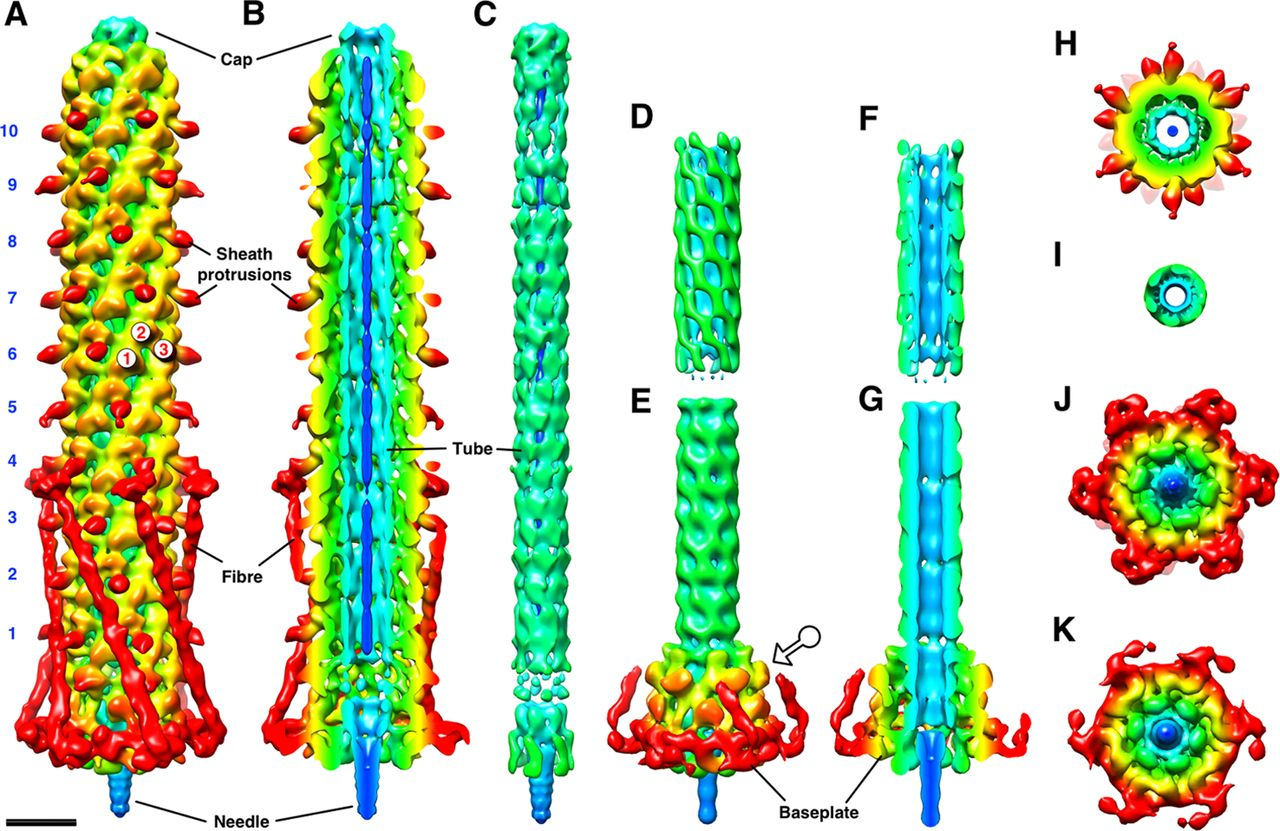
\includegraphics[width=0.49\textwidth, trim={256 143 0 7}, clip]{/Users/joehealey/Documents/Warwick/PhD/Thesis/chapters/intro/img/afp_map.jpg}} &
            \raisebox{-.5\height}{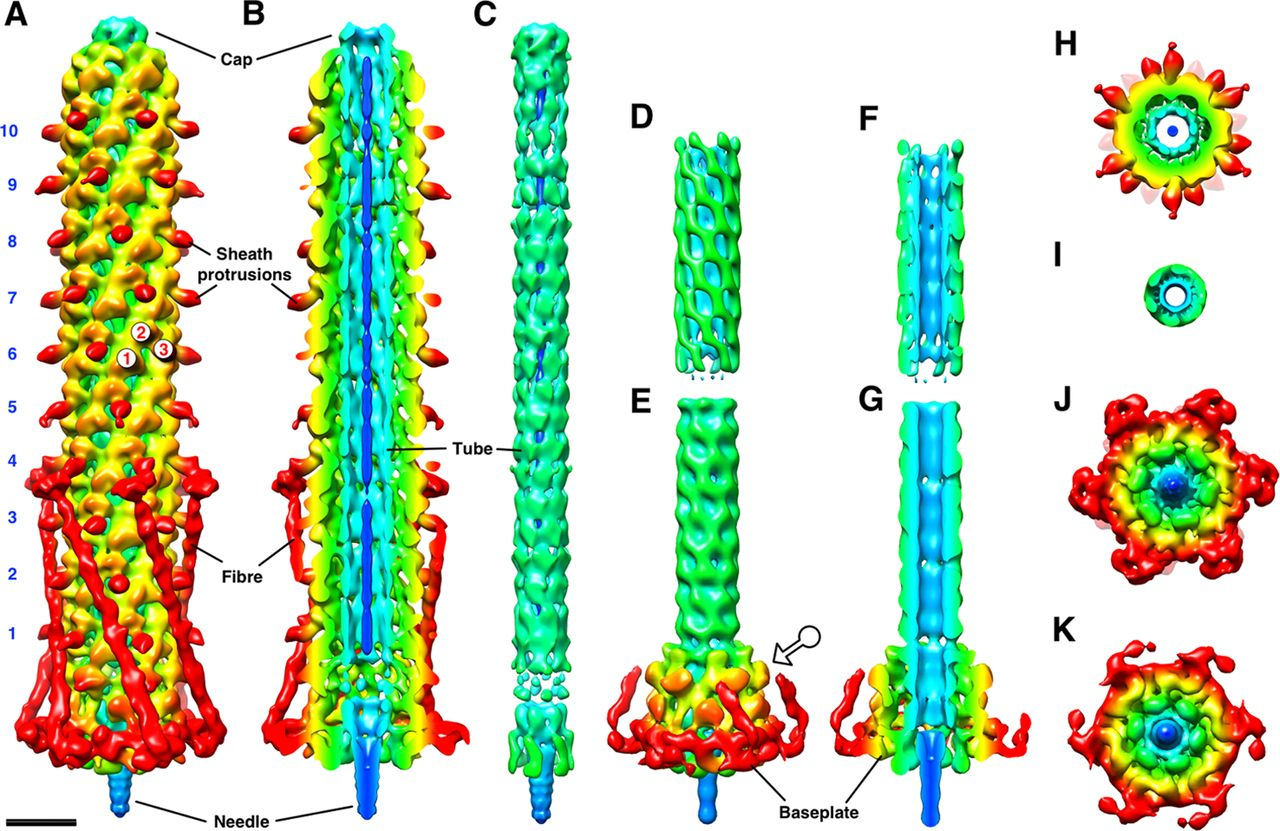
\includegraphics[width=0.49\textwidth, trim={255 55 0 90}, clip]{/Users/joehealey/Documents/Warwick/PhD/Thesis/chapters/intro/img/afp_map.jpg}} \\
                                  
            \raisebox{-.5\height}{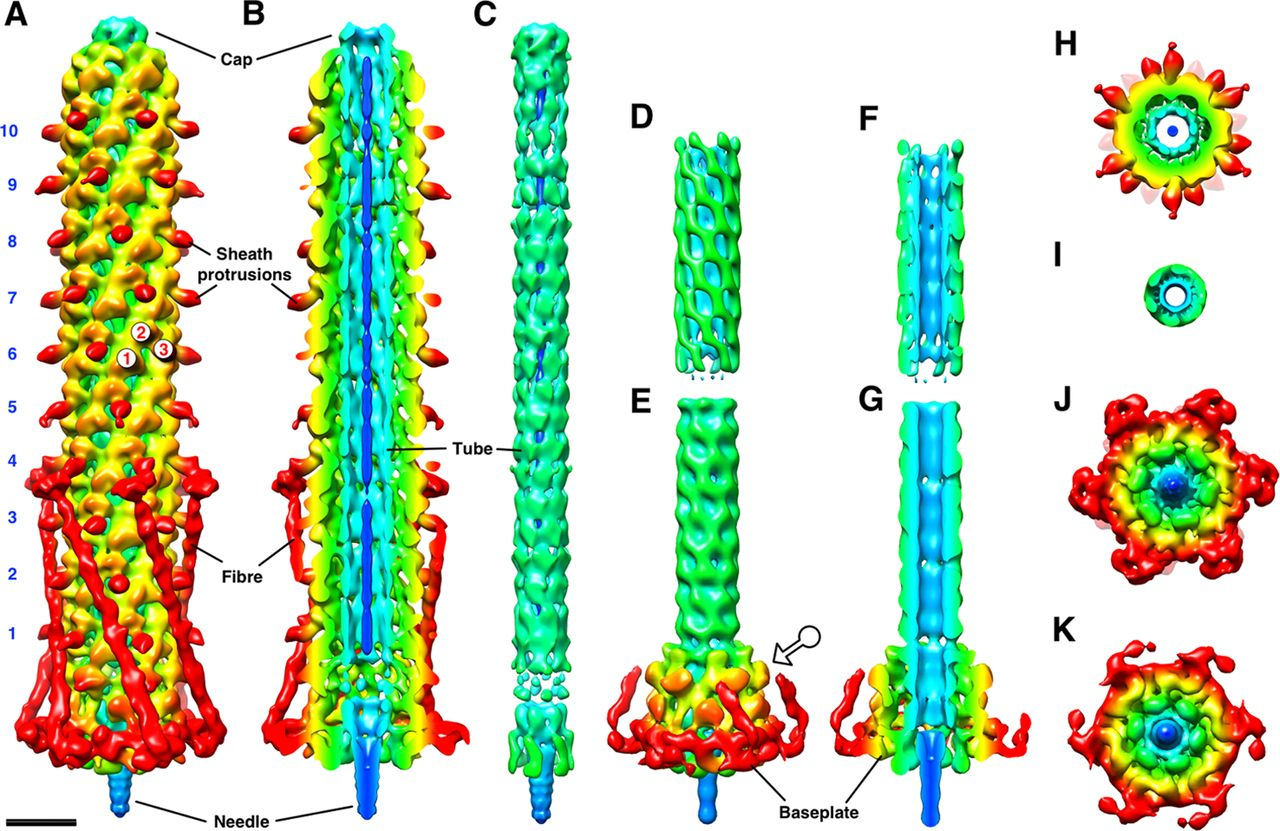
\includegraphics[width=0.49\textwidth, trim={256 120 0 60}, clip]{/Users/joehealey/Documents/Warwick/PhD/Thesis/chapters/intro/img/afp_map.jpg}} &
            \raisebox{-.5\height}{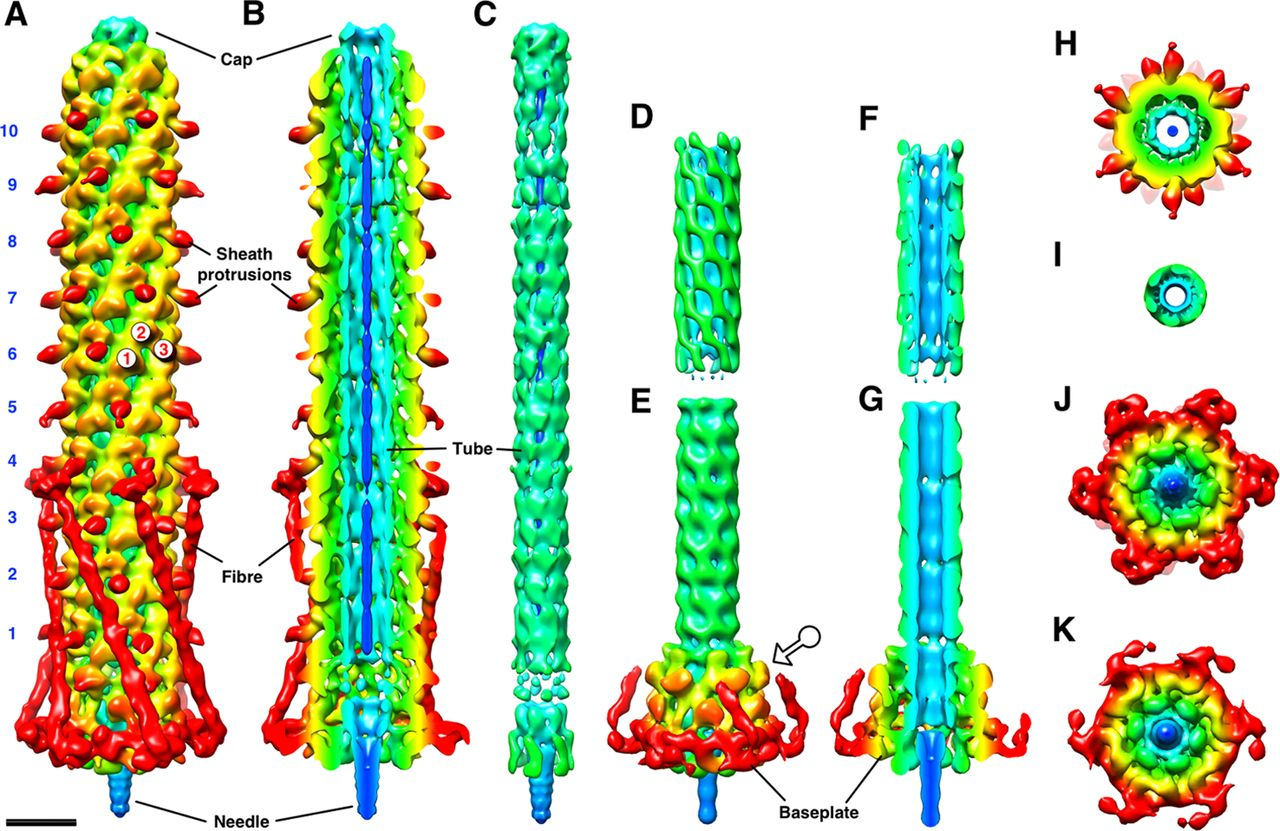
\includegraphics[width=0.49\textwidth, trim={255 0 0 150}, clip]{/Users/joehealey/Documents/Warwick/PhD/Thesis/chapters/intro/img/afp_map.jpg}} \\
     \end{tabular}
            \put(-141,90){\obscure{1cm}{1cm}}
            \put(-265,90){\obscure{1cm}{1cm}}
            \put(-141,-20){\obscure{1cm}{1cm}}
        \captionsetup{singlelinecheck=off, justification=centering, font=footnotesize, aboveskip=10pt}
        \caption{}
        \label{afp2}
        \end{subfigure}%
}\vfill
    \hbox{%
        \begin{subfigure}[t]{0.58\textwidth}
            \centering
            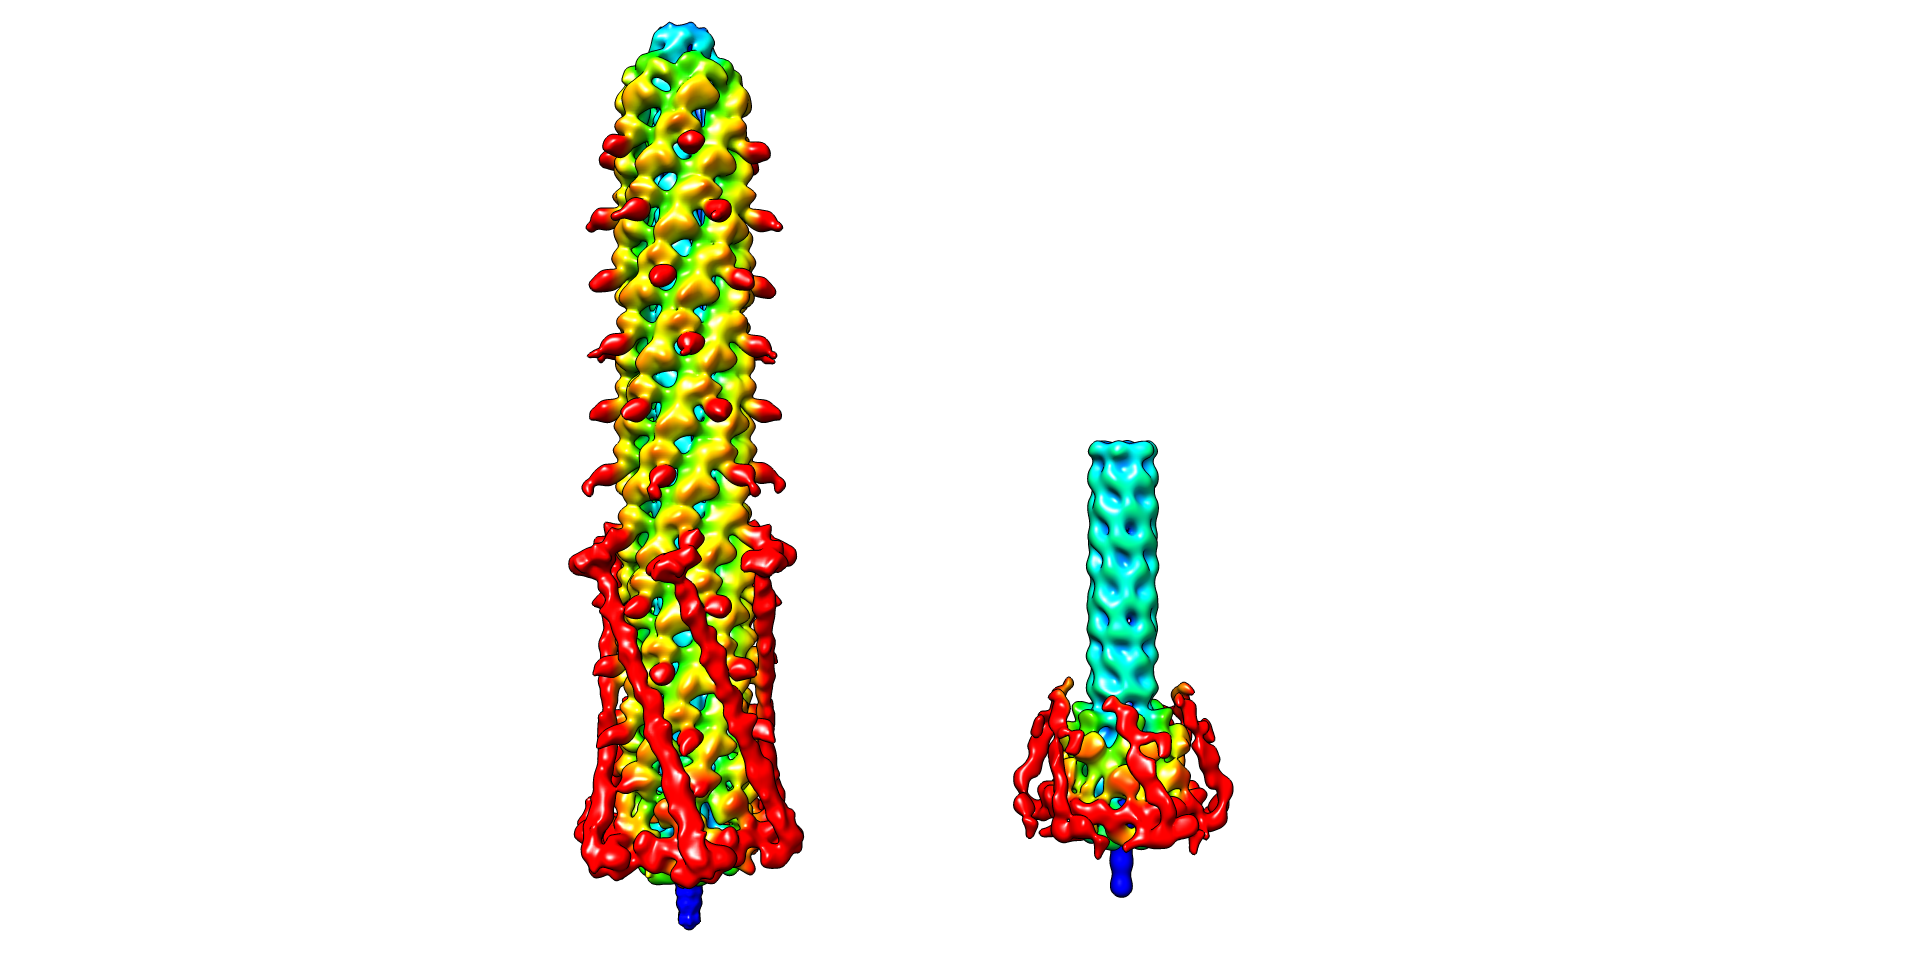
\includegraphics[width=\textwidth, trim={105 7 68 52}, clip]{/Users/joehealey/Documents/Warwick/PhD/Thesis/chapters/intro/img/afp_map_reconstructed.png}
            \captionsetup{singlelinecheck=off, justification=centering, font=footnotesize, aboveskip=15pt}
            \caption{}
            \label{afp3}
        \end{subfigure}%    
  }\cr
}
	\captionsetup{singlelinecheck=off, justification=justified, font=footnotesize, aboveskip=10pt}
	\caption[Antifeeding prophage Electron Density maps from \cite{Heymann2013}]{\textsc{\normalsize The structures of the Antifeeding prophage from \cite{Heymann2013}.}\vspace{0.1cm} \newline \textbf{(A)} The reconstructed 20 \AA{} electron density map for the \emph{S. entomophila} Antifeeding prophage, based upon \cite{Heymann2013}, and reproduced independently from the deposited data under EMDB-2419. All panels in this image are coloured by the distance in \AA{}ngstroms from the centre of rotational symmetry (blue $\leq$ 20\AA \ to red $\leq$100 \AA). Some features of note include the dark red sheath protrusions and the very well defined putative tail fibres folded back against the tube. \textbf{(B)} Various orthogonal views of the tube baseplate/spike and inner core. Note, in particular, a density in the lumenal space in the top left panel. Adapted and reproduced from \cite{Heymann2013}. \textbf{(C)} A ``Tube-Baseplate Complex" which was expressed without any exterior sheath proteins in the same study, revealing further detail of the baseplate complex and the inner sheath.}
	\label{afpstructure}
\end{figure}
}

Despite this extensive study, the EM map that was obtained, displayed in \vref{afpstructure}, is low resolution (at only 20 \AA), and only the gross architecture of the spike and tubes are reliably discernible. This was a substantial improvement over previous iterations however, as the group were able to correct an initial erroneous observation that the tube would have four-fold symmetry, when in actuality, it has six-fold \citep{Sen2010}. Despite this lower resolution, the Afp map does have some unique features, and even advantages over the atomistic R-type pyocin map. As with the other structures that have gone before, the mesh-like structure of the outer sheath is revealed in the obtained density, with the inner sheath visible through `fenestrations' in the outer sheath structure. A baseplate and spike complex is clearly visible, though with no strongly discernible features at this resolution. Attached to the baseplate however, are incredibly distinctive densities for the putative tail fibres, present in a kind of `docked' or `folded' conformation. The fact the tail fibres have been locked in to a prostrate position along the length of the tube, has likely stiffened them, allowing them to be imaged successfully without the averaging effect of tomography blurring them out, as is the case with the structure from \cite{Ge2015}. Indeed, in \vref{afp3}, the lack of the outer sheath stabilising the distal ends of the fibres has resulted in the commonly seen blurring effect. Even at a 20 \AA{} resolution, it is possible to identify a bulbous region at the distal ends of the tail fibres, which is consistent with the trimeric nature of other, more fully resolved, viral adhesion proteins.

Another striking feature of the Afp structure versus the R-type pyocin and the T4 phage, is that the outer sheath appears to more closely resemble that of T4, due to having long sheath protrusions (visible in dark red in \vref{afp1}), than it does the R-type pyocin. This structure, combined with the initial suspicion of four-fold symmetry lead \cite{Sen2010} to conclude that the Afps may represent an evolutionarily distinct sub-type of contractile tail structures. Whether or not this is valid in the context of the protrusions being unusual when compared to the R-type pyocin for example, is not clear without a fully resolved atomistic structure. It is clear that the argument from four-fold symmetry is erroneous in light of the more recent and higher resolution studies of \cite{Heymann2013} however. At present, there is no known functional relevance for these domains.
 
Finally, there is one particularly interesting feature of the EM densities obtained by Heymann and colleagues. In \vref{afp2}, in the top left inset panel, a dark blue density can be seen in the lumen of the central tube. This presents a couple of possible explanations. Perhaps the most likely explanation is that it is artifactual from the averaging process, given that this axial region would not move greatly during tomography, and would thus appear as a static, but blurred, part of the structure.

Alternatively, it is possible there is a structural or biological basis for these densities. As was mentioned in the review of T4, caudate structures are proposed to require a tail `tape measure' protein which extrudes along the length of the growing tail and triggers capping. In T4, this has been proposed to be gp29, and through deletion studies, a similar role was observed for Afp16 \citep{Rybakova2013, Abuladze1994, Katsura1987}. One current theory is that these tape measure proteins exert their effect by lying along the length of the interior of the tube, though there is sparse evidence for this particular mechanism. If this were the case, this density may well correspond to a tape measure protein.

Lastly, the Afps, like the PVCs are thought to package payload effector molecules in to the interior of the tail. This is an intriguing prospect, and would represent the first structural data that attests to this. Given the uniformity of the density along the length of the tube, and its width of only a few \AA{}ngstroms however, the former of these 3 theories seems like the most likely given the information at hand.

In summary, the Afps and PVCs are extremely similar, which is perhaps not unsurprising given their host's similar lifestyles as insect pathogens. However, as this section as highlighted, they are not without differences, corresponding to potentially drastic differences in selection pressure and deployment in the environment. Chief among the differences are the fact that the Afps are plasmid borne, and the PVCs aren't (though perhaps once were). A compelling explanation for significantly different selection pressures is the fact that Afps have been demonstrated to be extremely selectively toxic to only the New Zealand grass grub. The geographic isolation of New Zealand, known for its unusual flora and fauna, may point to a long co-evolution of \emph{S. entomophila} and \emph{C. giveni} which limits the host range. In the recent paper by \cite{Hurst2008}, AfpX was demonstrated to be toxic to the larvae of the Manuka beetle (\emph{Pyronata festiva}), another organism which is endemic to New Zealand, and has yet to be found elsewhere. \emph{Photorhabdus}, by contrast, has demonstrated wide ranging lethality to insects, and is found throughout the world. Lastly, the PVCs are present in various forms, scattered throughout \emph{Photorhabdus} genomes, and this alone has potentially lead to enormously different selection pressures (due to their paralogy), and potentially morphology - whereas \emph{Serratia} is limited to only 2 examples (and still only a single operon per genome).


\subsubsection{Of PVCs and Type VI Secretion Systems}\label{t6ss}
Now that the closest cousins of the PVCs have been discussed, in the form of the AFPs and R-type pyocins, moving back up in complexity brings us back to another well studied biological complex - the Type VI Secretion System (T6SS). \cite{Bonemann2010} were the first to draw parallels between the T6SS and the PVCs, realising that the contractile, puncturing mechanism of the system placed it in a `supergroup' of contractile injection systems.

 The T6SS is just one of a family of secretion systems which have come to be recognised in bacteria, as a mechanism for the organism to communicate with, and manipulate, the extracellular environment, including other organisms. At the time of writing, at least 9 ``Type \textbf{$x$}" secretion systems have been described (numbered in Roman numerals I to IX), each of which has been studied to a differing degree and there are great number of reviews covering some or all of them to date \citep{Dalbey2012,Chang2014a, Bleves2010, Desvaux2009, Abby2016, Costa2015, Goulet2004, Remaut2008, Gerlach2007, Abdallah2007, Green2015}. The ``Type \textbf{$x$}" secretions systems are specialised bacterial structures, and are distinct from the Sec and Tat secretion systems which are present in all 3 domains of life, meaning bacteria exhibit a dizzying array of secretion mechanisms \citep{Green2015}. Discussions of secretion systems are quite `murky waters' however, as they are not all related, despite being named as if they are `shades of grey' with respect to each other. As the details of all the secretion systems are not wholly pertinent to discussions of the PVCs, the depth will be left to the aforementioned reviews. This section will highlight the different types and diversity of known secretion systems, and will then proceed to cover the Type VI secretion system in depth.

\myparagraph{The ``Type \textbf{$x$}" Secretion System repertoire}
Briefly, the T1SS, is a translocator comprised of 3 proteins which is able to secrete a wide variety of bacterial proteins with a wide size range, the one of the largest being the LapA adhesion protein from \emph{Pseudomonas fluorescens}, at an impressive 520 kDa \citep{Boyd2014}. One of the most commonly transported proteins are toxins of the RTX family \citep{Delepelaire2004}. Unlike the other secretion systems, Type I is related to the general class of ABC transporters which are ubiquitous efflux pumps for antibiotics and other small molecules, and is entirely independent of the Sec system, not requiring a first translocation of cargo to the periplasm, though cargoes do require a chaperone.

The Type II Secretion system (T2SS) is a common Gram negative secretion system, and has been studied extensively in a number of human pathogens including \emph{Vibrio} and \emph{Pseudomonas}, though it is not ubiquitously present in Gram negatives \citep{Douzi2012}. The system can be divided in to 4 primary components, though the structure as a whole is a large multipartite protein complex. The inner membrane complex and outer membrane complex are connected by a `pseudopilus' spanning the periplasm, so called as it is made up of a number of proteins resembling pilins \citep{Korotkov2012}. Finally, a crucial hexameric secretion ATPase is associated with the inner membrane complex, and is responsible for the synthesis and dismantling of the pilins, which provides the mechanistic basis for secretion \citep{Lu2013}. Type II is Sec or Tat dependent, and exports a variety of protein cargoes, which often include toxins and degradative enzymes such as proteases and lipases associated with bacterial infection \citep{Korotkov2012}.

An unusual version of a secretion system, and another very well studied apparatus, the Type III Secretion System is quite similar to a PVC in its role as an anti-eukaryotic needle complex delivery system. Homologous to the basal body of the bacterial flagellum \citep{Aizawa2001}, the T3SS is another molecular syringe, but membrane bound. The Type III is used by bacteria to directly inject effector proteins in to the interior of target eukaryotic cells, making it a potent and widely utilised virulence factor \citep{AbuHatab1998} - with examples having been found in \emph{E. coli}, \emph{Shigella}, \emph{Salmonella}, \emph{Vibrio}, \emph{Burkholderia}, \emph{Yersinia}, \emph{Pseudomonas}, as well as a number of plant-associated species such as \emph{Rhizobium}, \emph{Erwinia}, \emph{Ralstonia} and \emph{Xanthomonas}, and more besides. By forming a continuous pore, through the needle bore, from the cytosol of the bacterium to the target cell, Type III is completely Sec/Tat independent. The similarity to the flagella continues in the needle body, as this is homologous to the flagella hook \citep{Lane2007}. Comparable in complexity to the flagella also, the T3SS is comprised of around 30 distinct proteins, making the T3SS among one of the most intricate secretion systems \citep{Green2015}.

Like the T3SS, the Type IV Secretion System is a relative of another fundamental bacterial `appendage' - the conjugation pilus, used by bacteria to exchange genetic material. Unlike the conjugation machinery however, the T4SS is capable of translocating protein (as well as nucleic material). The Type IV system was discovered originally in \emph{Agrobacterium tumefaciens}, the long-used tool for genetic manipulation of plant species, and is the mechanism by which the bacterium actually exerts its modifying effects. Thus, the \emph{A. tumefaciens} system in particular, has become the model for T4SS structure and function studies \citep{Bundock1995}. As with the Type III, the `injectisome' nature of the T4SS means that it is Sec/Tat independent. However, there are competing theories as to whether the T4SS simply acts as a harpoon, to pull 2 cells in to close register, and translocation occurs in a still as-yet-undetermined manner, or actually forms a continuous channel from cytosol to cytosol, as in the T3SS \citep{Christie2005, Green2015}.

Unique among all the secretion systems, The Type V Secretion System is an auto-transporter, rather than a channel for other proteins (though it is capable of exporting others as well in some cases), and requires no ATP to function \citep{Thanassi2005}. Proteins that comprise the T5SS class contain a C-terminal region which inserts into the outer membrane (after translocation via Sec), forming a $\beta$-barrel, and they then proceed to translocate the N-terminal passenger effector domain, which is proteolytically cleaved. The $\beta$-barrel remains in the outer membrane until it is lost or recycled, potentiating the passage of other substrates, once the passenger domain is no longer causing an obstruction. Continuing the theme from the other secretion systems, most known T5SS secreted proteins are virulence factors and host modulators \citep{Green2015}.

Skipping over the Type 6 for the moment, in favour of a more full review in this section, the Type VII secretion system is unlike the other secretion systems mentioned so far, as it (to date) has only been found in Gram positive bacteria such as the \emph{Corynebacteria} and \emph{Actinobacteria}, and most famously in the \emph{Mycobacteria} \citep{Ates2016}. Gram positive bacteria, due to their (typically) single cell membrane, and thickened cell wall, have different challenges to overcome when secreting molecules in to the extracellular milieu \citep{Green2015}. It is thought that the T7SS is widespread amongst Gram positives, with Type VII-like operons and orthologues having been detected in \emph{Staphylococcus aureus}, and \emph{Bacillus subtilis}, the well known model organism for Gram positives. The structure and function of the complex and its constituent proteins are not yet well understood. There is a large inner membrane complex, formed of at least 5 distinct proteins, which is thought to provide a channel for substrates, though there are a number of additional proteins for which roles have not yet been elucidated. Since the formation of a pore in the membrane would not allow substrate passage beyond the interior face of the cell wall, it seems likely that some or all of these remaining proteins serve to facilitate this last hurdle in some way. Though extremely distant in terms of any genetic relation (if any), there is an interesting parallel between the PVCs, and the T7SS in \emph{M. tuberculosis}; namely, that the \emph{Mycobacteria} harbour up to 5 T7SSs, as \emph{Photorhabdus} habours up to 6 PVCs, and not all of these are present in every genome of the species \citep{Bottai2017}. The T7SS is known to function mostly (though not entirely) in virulence, and this potentially speaks to the same diversification seen in the PVCs, honing multiple copies of highly effective virulence factors to become a more effective pathogen, or cope with varying environmental conditions.

Historically, the Type VIII system has been referred to as the `extracellular nucleation-precipitation pathway' (ENP) and the switch to T8SS was proposed by \cite{Desvaux2009}. The structure of the T8SS was resolved by \cite{Goyal2014}, and comprised a fairly typical looking membrane 36-strand $\beta$-barrel which is embedded in the outer membrane. The T8SS, therefore, is Sec/Tat dependent. Unlike the majority of the other secretion systems, the Type VIII is thought to be limited to a single substrate. It is responsible for secreting proteins known as `curli' - a primary component of the extracellular matrix of many \emph{Enterobacteriaceae} \citep{Barnhart2010}.

The Type IX Secretion System is one of the most recently discovered secretion systems with only a single structurally resolved component. To date, it has only been detected in certain species of the \emph{Bacterioidetes} phylum, after being originally discovered in the oral pathogen \emph{Porphyromonas gingivalis}. The T9SS has been demonstrated to be implicated in 2 distinct lifestyle roles, both gliding motility and as a pathogenic virulence factor/weapon, though with unknown functional bases. It is dependent on the Sec system, providing only carriage across the outer membrane. Originally termed the PorSS system, 18 proteins are known to be essential, but roles for all of them remain elusive, while as many as 29 proteins are hypothesised to be involved in some way, making the T9SS comparable in complexity to the Type III and Type VI \citep{Lasica2017a}


So, finally returning to the Type VI secretion system, as with the T4 capsid, this section is not going to dwell extensively on the membrane associated apparatus of the Type 6 Secretion System, since the PVCs appear to be secreted/released by lysis, and thus contain no analogous structures (and the membrane complex is still not well understood). Instead the similarities of the PVCs and the T6SS in terms of their putative translocation role and thus their spikes and tubes (i.e. as contractile nanomachines) will be the focus.

The T6SS has been identified in about 25\% of all Gram negative sequences \citep{Basler2015a}, and despite being the most recently discovered secretion system (first being dubbed the T6SS in 2007) \citep{Nguyen2018, Pukatzki2007, Cascales2012}, it has rapidly become quite well studied, with a significant amount of structural resolution completed to date \citep{Mougous2006a}. It has been shown that the T6SS is encoded by a highly conserved 13 gene cassette, which forms the core of the system, with a number of accessory proteins. The presence of these accessory proteins can vary by organism, but are typically well conserved when they are found \citep{Basler2015a}.

Among all the secretion systems, the Type VI is unique in a couple of primary ways. Firstly, it is the only secretion system with a contractile mechanism, as with T4 and the pyocins etc., as well as being the only system which delivers effectors to both other bacteria, and eukaryotic targets. Thus, the T6SS is an intricate but highly versatile nanosyringe complex - essentially an ``upside down myophage in the membrane" - and is employed by a large number of bacteria in their pathogenic, but also community roles \citep{Russell2014}. 


\vspace{0.1cm}
\begin{figure}[h]
\centering
    \begin{subfigure}[b]{0.481\textwidth}
        \centering
        {%
\setlength{\fboxsep}{0pt}%
\setlength{\fboxrule}{1pt}%
        \fbox{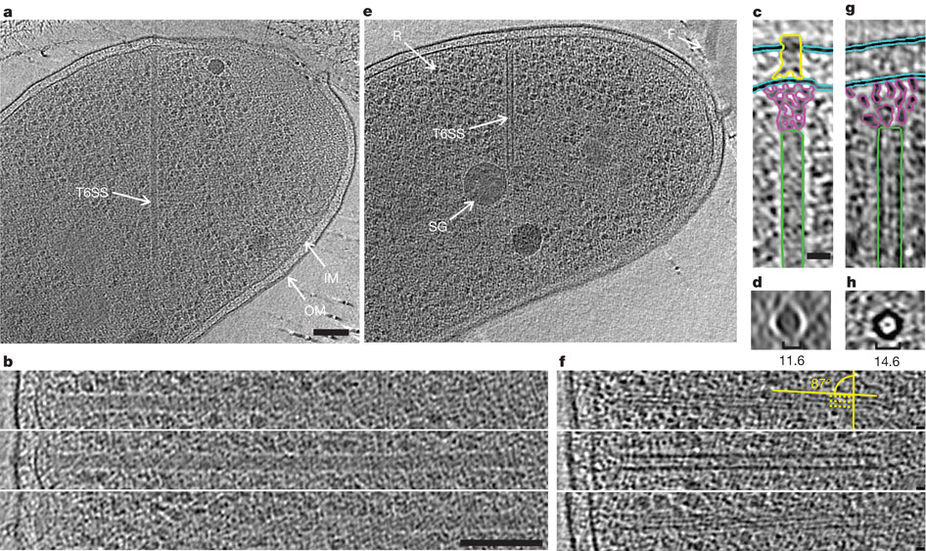
\includegraphics[width=\textwidth, trim={0 230 200 20}, clip]{/Users/joehealey/Documents/Warwick/PhD/Thesis/chapters/intro/img/t6ss_in_cell.jpg}}
            }%
    \end{subfigure}%
    \begin{subfigure}[t]{0.499\textwidth}
        \centering
        {%
\setlength{\fboxsep}{0pt}%
\setlength{\fboxrule}{1pt}%
        \fbox{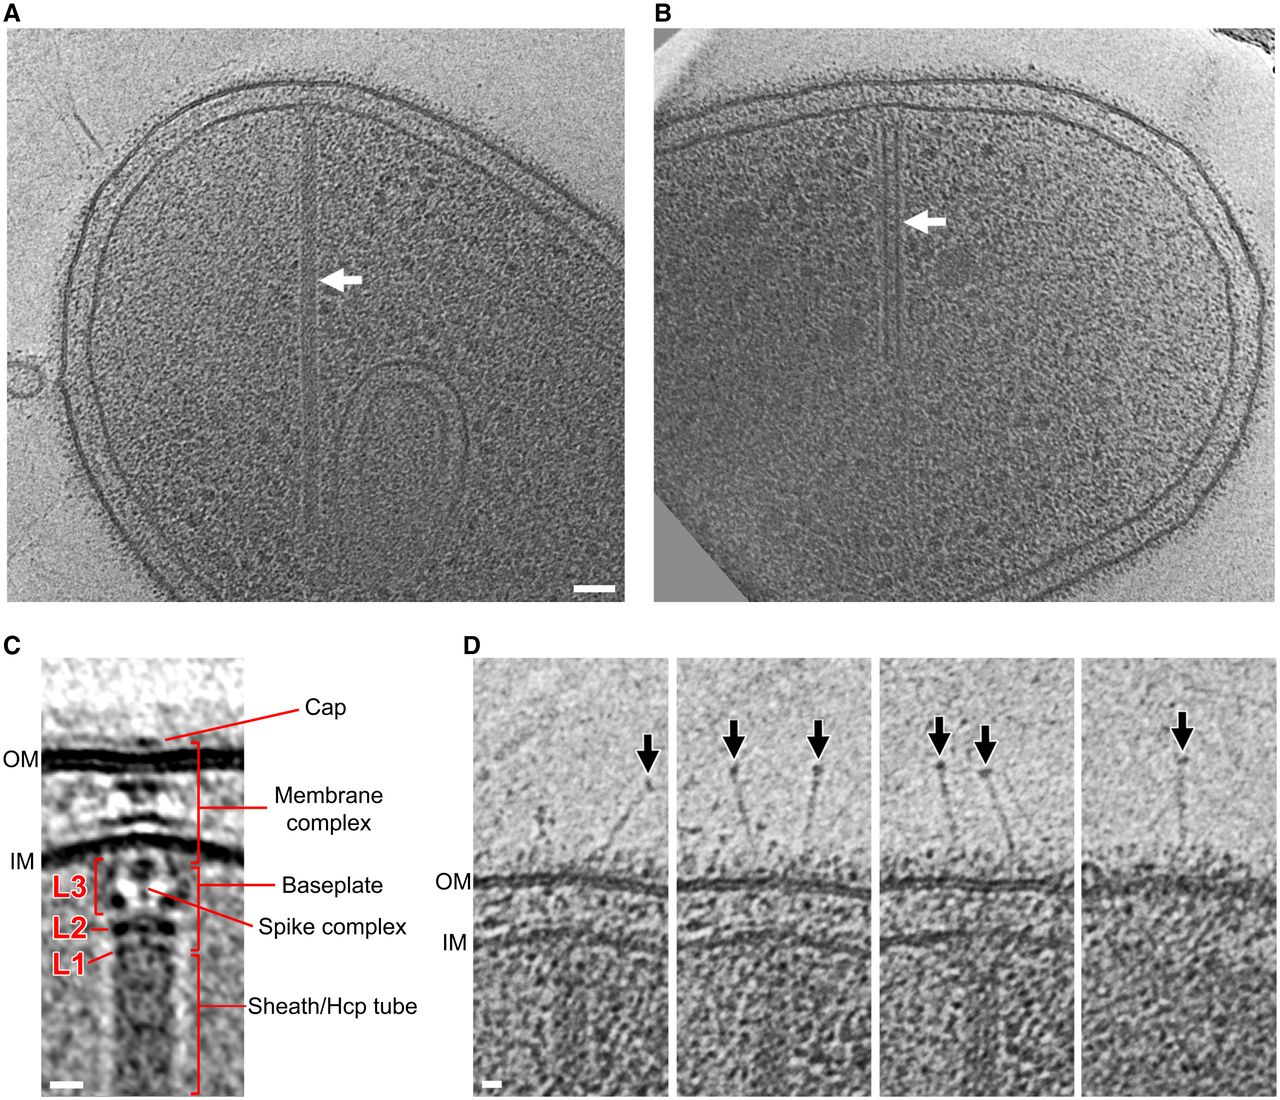
\includegraphics[width=\textwidth, trim={0 1 50 160}, clip]{/Users/joehealey/Documents/Warwick/PhD/Thesis/chapters/intro/img/t6ss_annotated}}
        }%
        \end{subfigure}%
	\captionsetup{singlelinecheck=off, justification=justified, font=footnotesize, aboveskip=10pt}
	\caption[Electron micrographs of the Type VI Secretion System]{\textsc{\normalsize Electron Micrographs of the Type VI Secretion System.}\vspace{0.1cm} \newline The left panel shows 2 EMs of the T6SS, and displays the enormous magnitude and variability in size of the tube complex, in the left most inset, the T6SS is labelled. In the right inset, the T6SS is labelled again, along with putative ribosomes (R), a flagellum (F), storage granule (SG), and the inner and outer membranes (IM/OM) Adapted and reproduced from \cite{Basler2012}. The right hand panel shows an annotated close up of the T6SS membrane complex. Labelled are the Inner and outer membranes (IM/OM), cap, membrane complex, tube, spike complex, baseplate, and the black arrows in the left most tryptic identify `antennae', purported to be the T6SS equivalent of phage tail fibres. L1-L3 demarcate different layers of EM density. Adapted and reproduced from \cite{Chang2017}.}
	\label{t6ssEMs}
\end{figure}


Though its role in pathogenesis was determined first by \cite{Pukatzki2006} whereby the T6SS locus of \emph{Vibrio cholerae} was demonstrated as enabling the bacterium to resist predation by the model amoeba species \emph{Dictyostelium discoideum}, the T6SS is deployed predominantly against prokaryotic targets \citep{Green2015, Russell2014, Hood2010}. A wide variety of roles for the T6SS have been postulated, both in antagonism (which is well documented) and in synergism. The diversity of competition against which the T6SS might be deployed `in the wild' is thought to underscore the rampant diversity that is seen between homologues. Furthermore, the need for competition between extremely closely related species and even strains, is driving the underlying selective pressure that has resulted in an enormous variety of Type VI effectors \citep{English2012, Russell2012}. The effector/immunity protein pairs that typify Type VI effectors have been suggested to act in a number of subtle ways, given this diversity. A rather ingenious mechanism has been proposed, wherein target cells which harbour a cognate immunity protein for a given toxin, utilise the toxin-immunity complex as a signalling molecule. Thus, those which have the correct immunity protein receive a signal, whereas those that don't, receive an antagonistic `message' - as if the bacteria are mailing each other `booby trapped' messages \citep{Russell2014}. Among other synergistic roles, the T6SS has been implicated in: the determination of self vs. non-self in \emph{Proteus mirabilis} \citep{Gibbs2008, Wenren2013}; triggering `assisted suicide' in phage infected cells inter-cellularly, in a manner analogous to that shown for `classic' Toxin-Antitoxin systems \citep{Hazan2004}; and as a method for overcoming the outer membrane to deliver cell wall remodelling factors which have been shown in other systems to `resuscitate' neighbouring cells from viable-but-non-cultureable states \citep{Downing2005, Mukamolova2006}.



\begin{figure}[p]
\thisfloatpagestyle{augment}
\centering
\tabskip=0pt
\valign{#\cr
\hbox{%
    \begin{subfigure}[t]{0.42\textwidth}
        \centering
         \begin{tabular}{c}
            \rotatebox{90}{\raisebox{-.5\height}{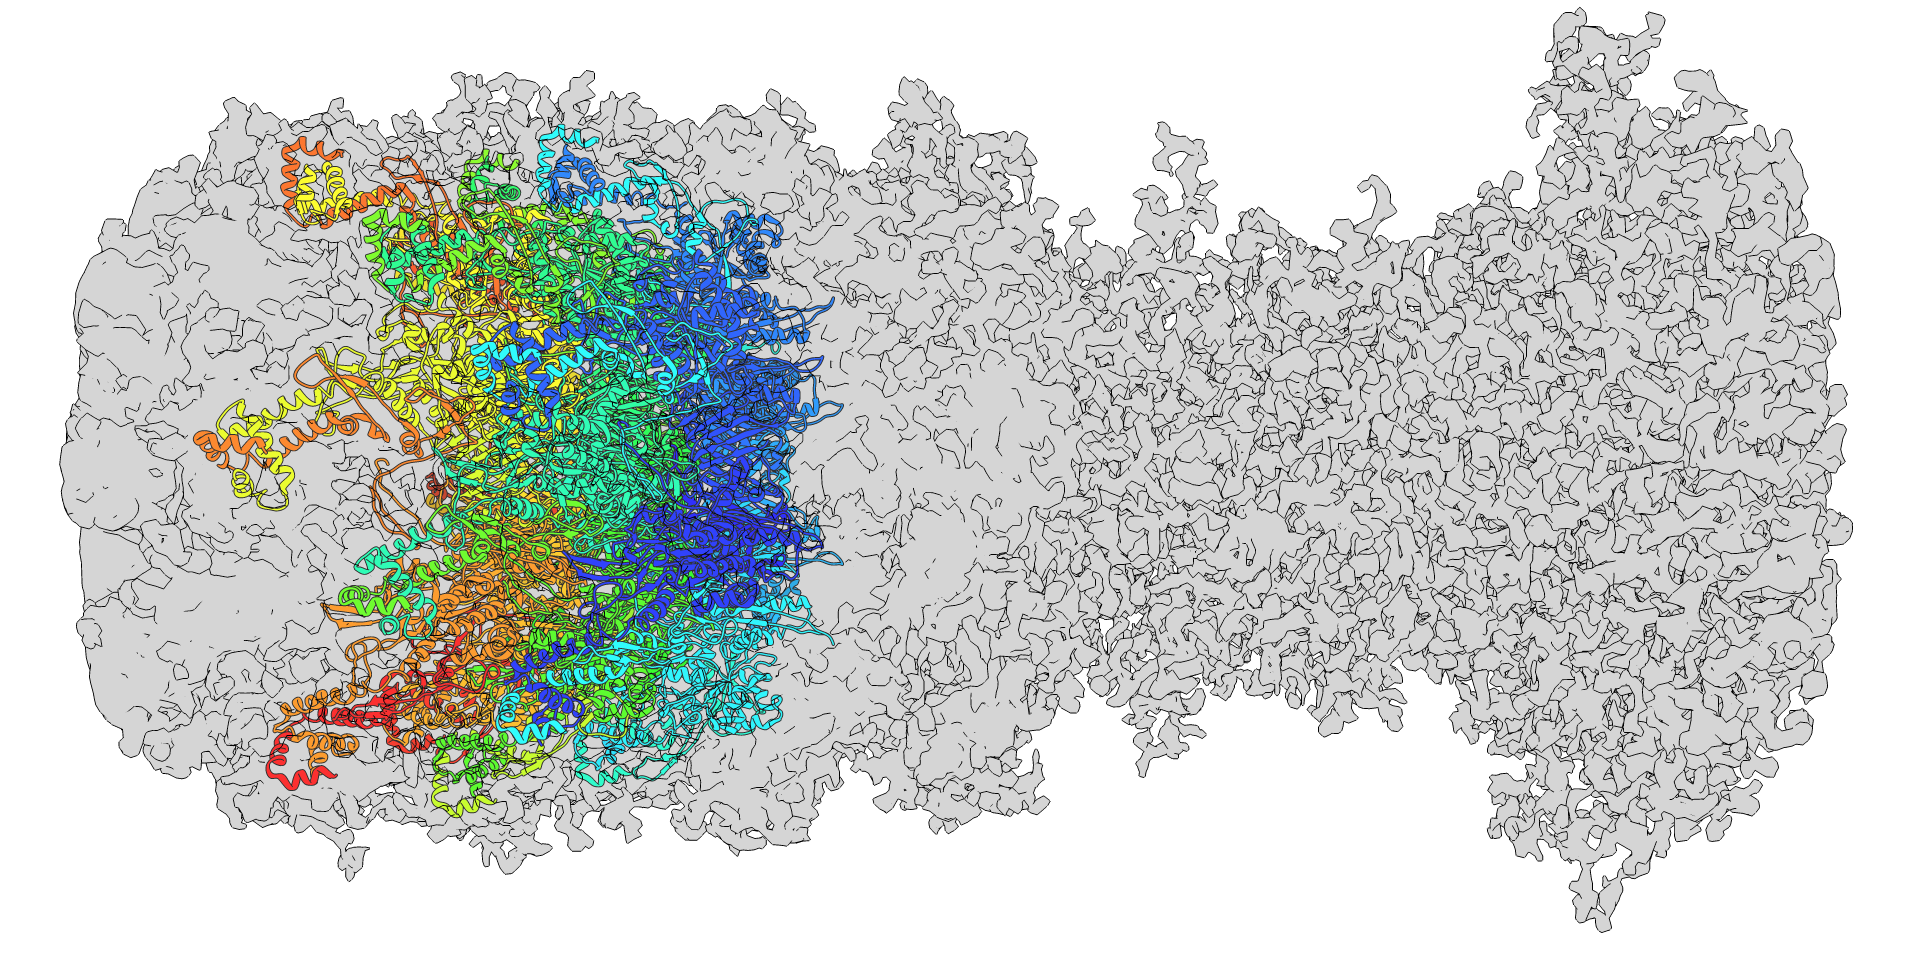
\includegraphics[width=1.65\textwidth, trim={20 0 10 0}, clip,]{/Users/joehealey/Documents/Warwick/PhD/Thesis/chapters/intro/img/t6ss_distal_grey_flat.png}}} \\
            \rotatebox{90}{\raisebox{-.5\height}{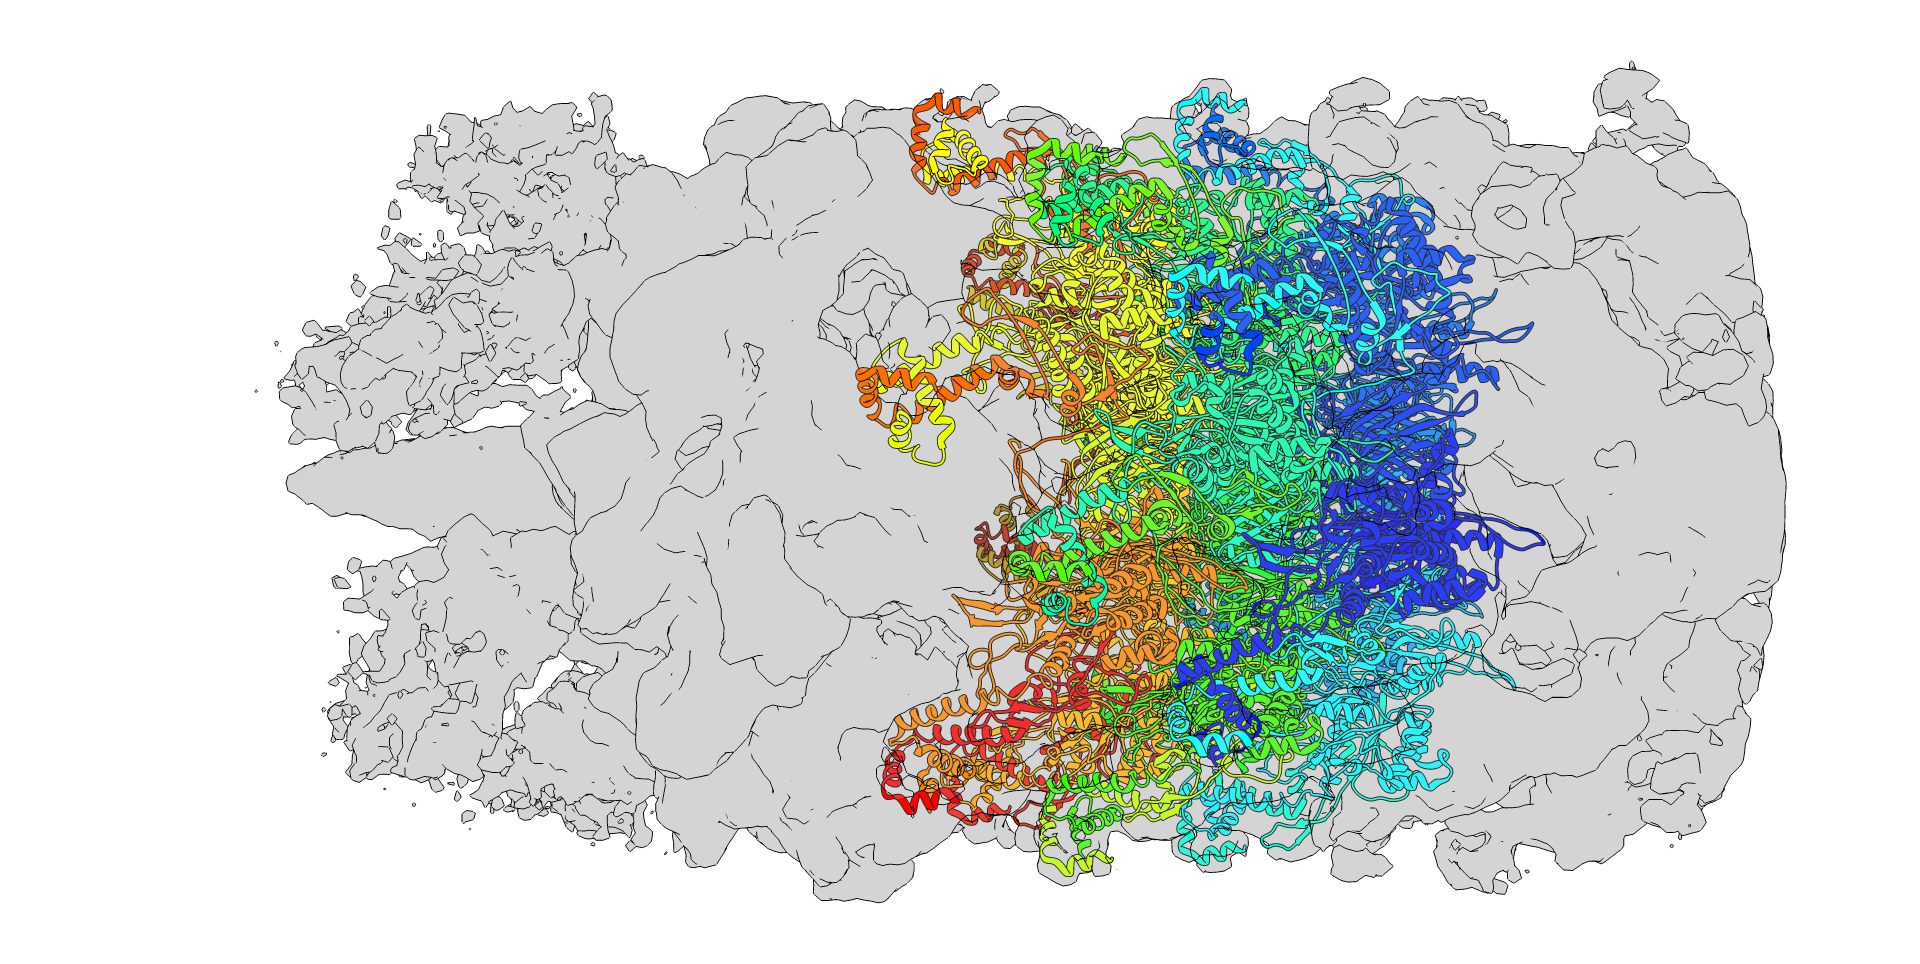
\includegraphics[width=1.38\textwidth, trim={30 0 30 0}, clip]{/Users/joehealey/Documents/Warwick/PhD/Thesis/chapters/intro/img/t6ss_proximal_grey_flat.png}}} \\
          \end{tabular}
         \put(-171,-15){
                 \rotatebox{-85.5}{
                     \obscure[gray]{0.02cm}{5.1cm}\obscure{0.5cm}{5.1cm}\obscure[gray]{0.02cm}{5.1cm}}
                 }
%         \put(-129,-25){\rotatebox{5}{\footnotesize$x$ hundred nanometres \{}}
        \captionsetup{singlelinecheck=off, justification=centering, font=footnotesize, aboveskip=10pt}
        \caption{}
        \label{tss1}
    \end{subfigure}%
}\cr
\noalign{\hfill}%
\hbox{%
    \begin{subfigure}{0.58\textwidth}
        \centering
        \vspace{1cm}
          \begin{tabular}{lr}
            \raisebox{-.5\height}{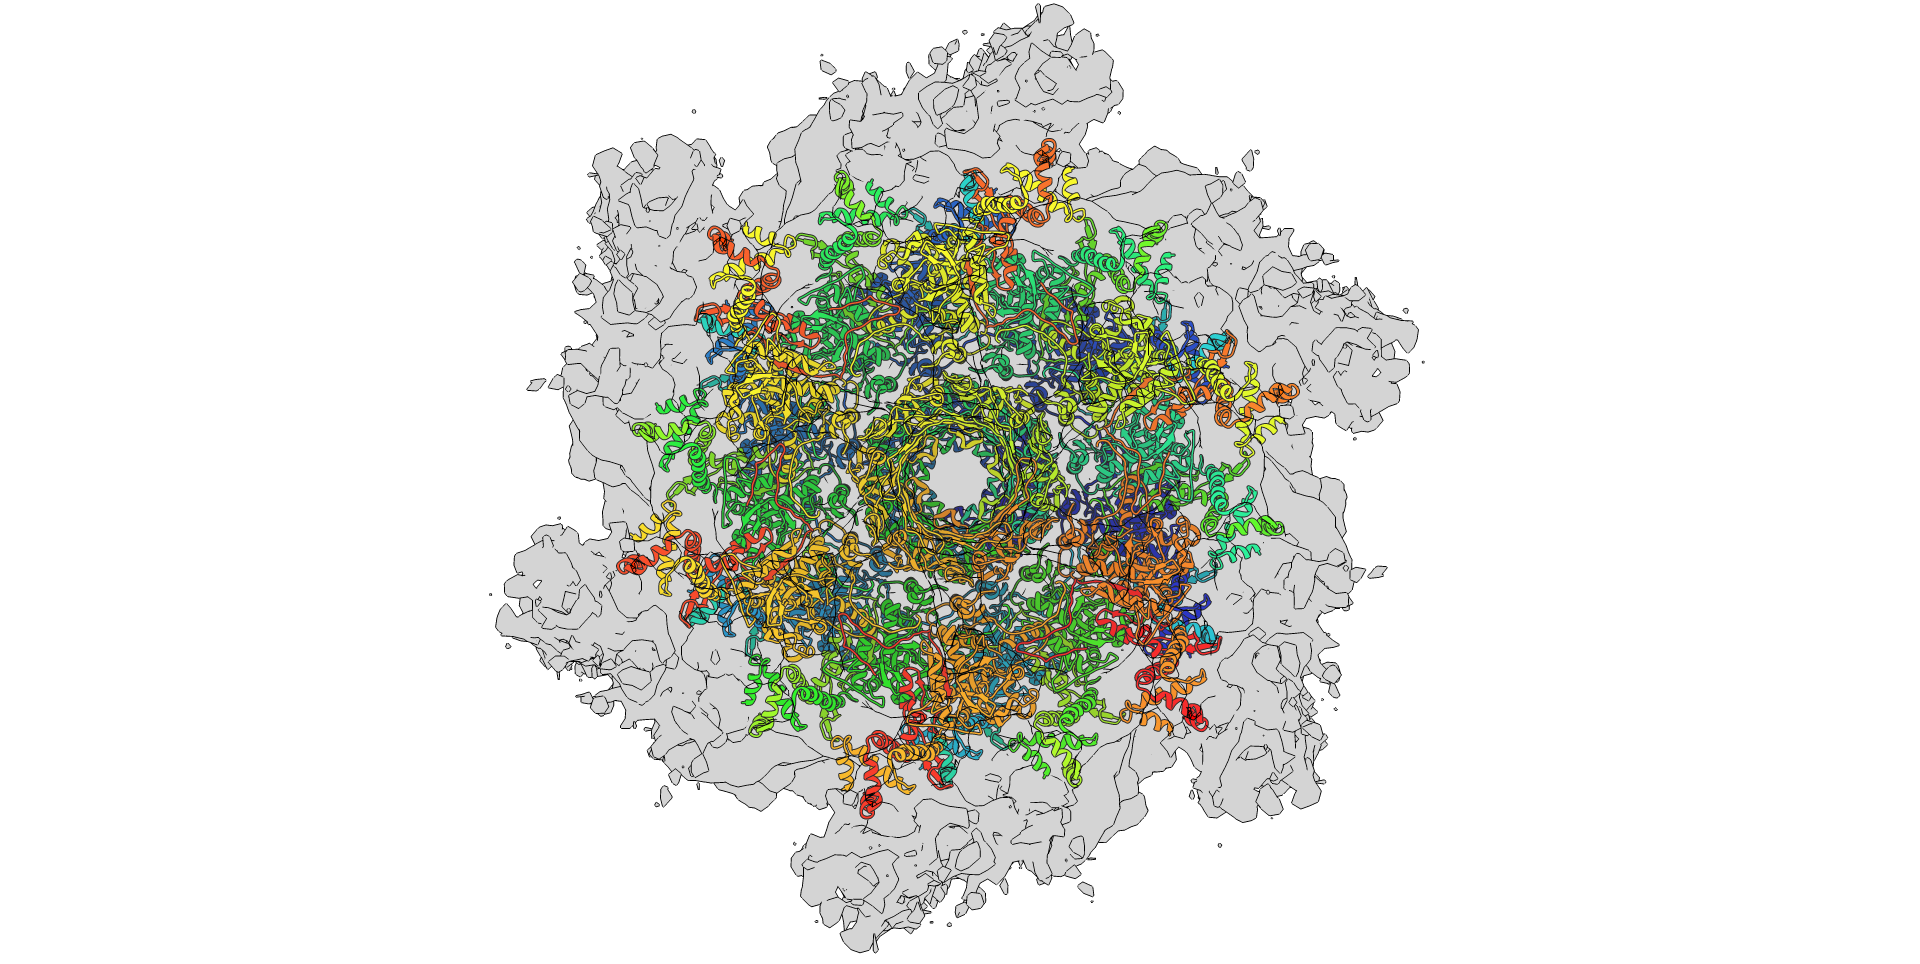
\includegraphics[width=0.5\textwidth, trim={55 0 55 0}, clip,]{/Users/joehealey/Documents/Warwick/PhD/Thesis/chapters/intro/img/t6ss_proximal_grey_flat_bottom.png}} &
            \raisebox{-.5\height}{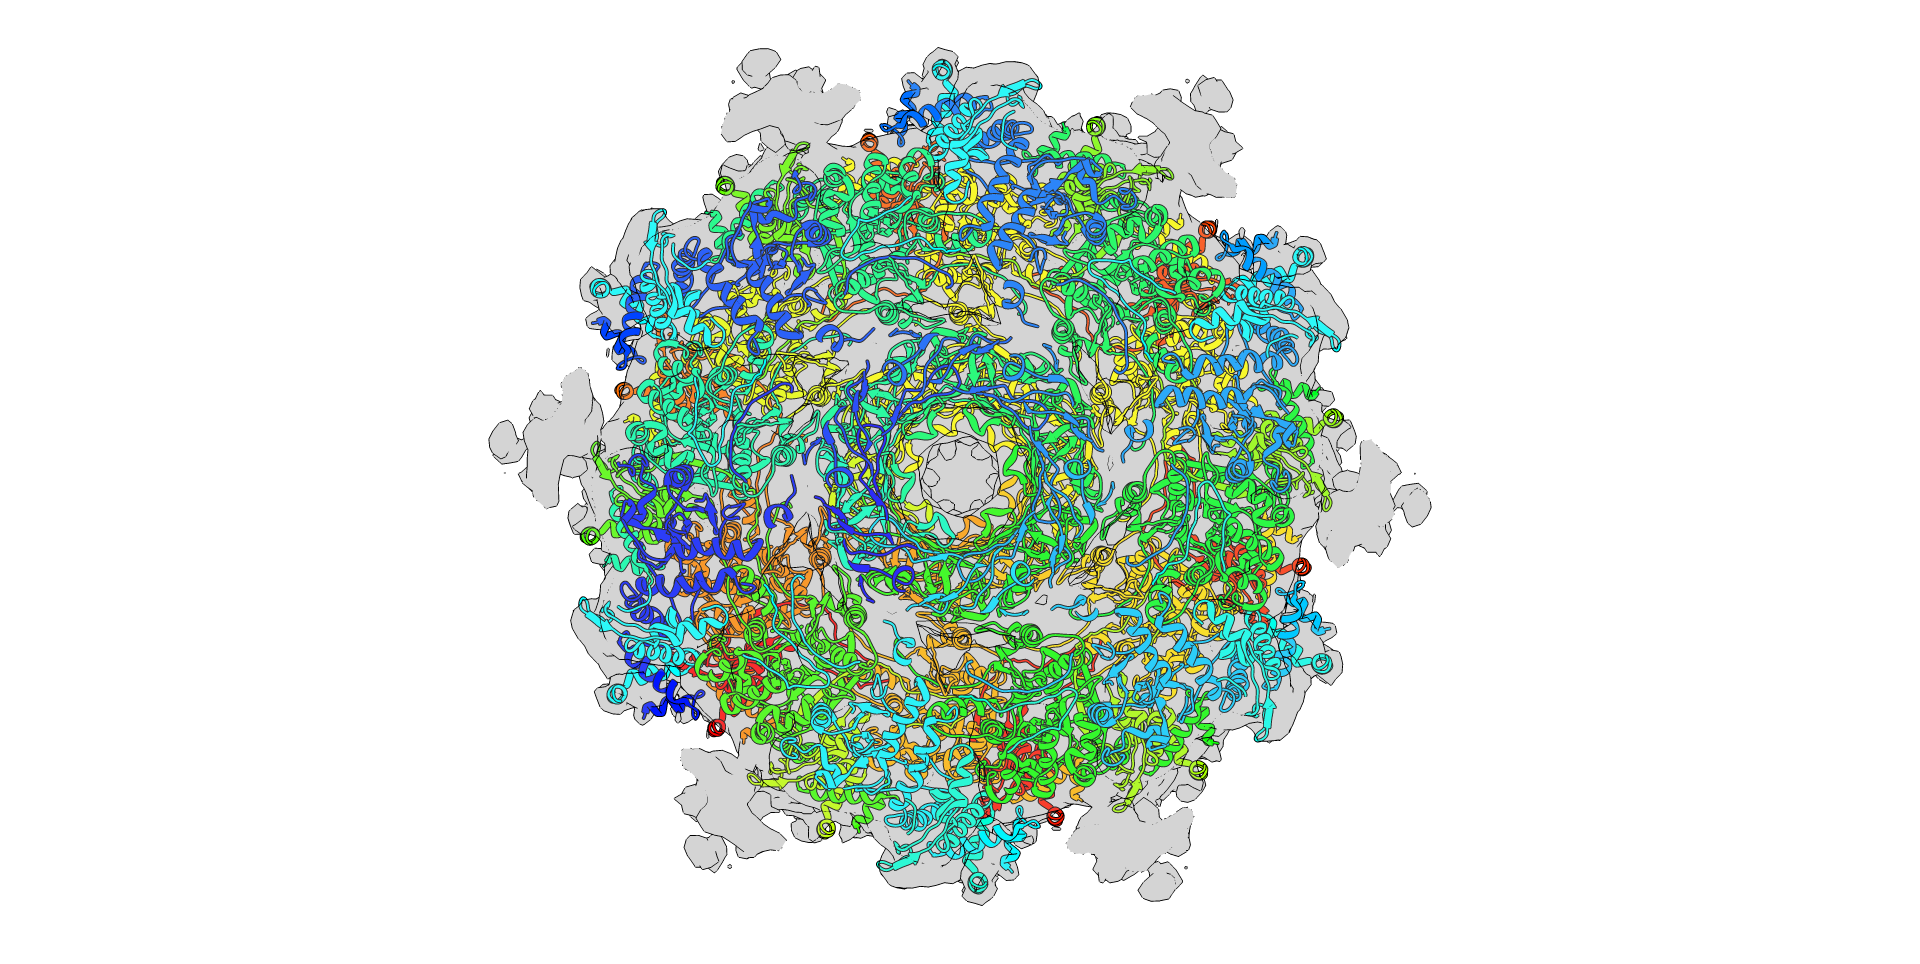
\includegraphics[width=0.5\textwidth, trim={55 0 55 0}, clip]{/Users/joehealey/Documents/Warwick/PhD/Thesis/chapters/intro/img/t6ss_proximal_grey_flat_topslice.png}} \\[2ex]
            \multicolumn{2}{c}{\raisebox{-.5\height}{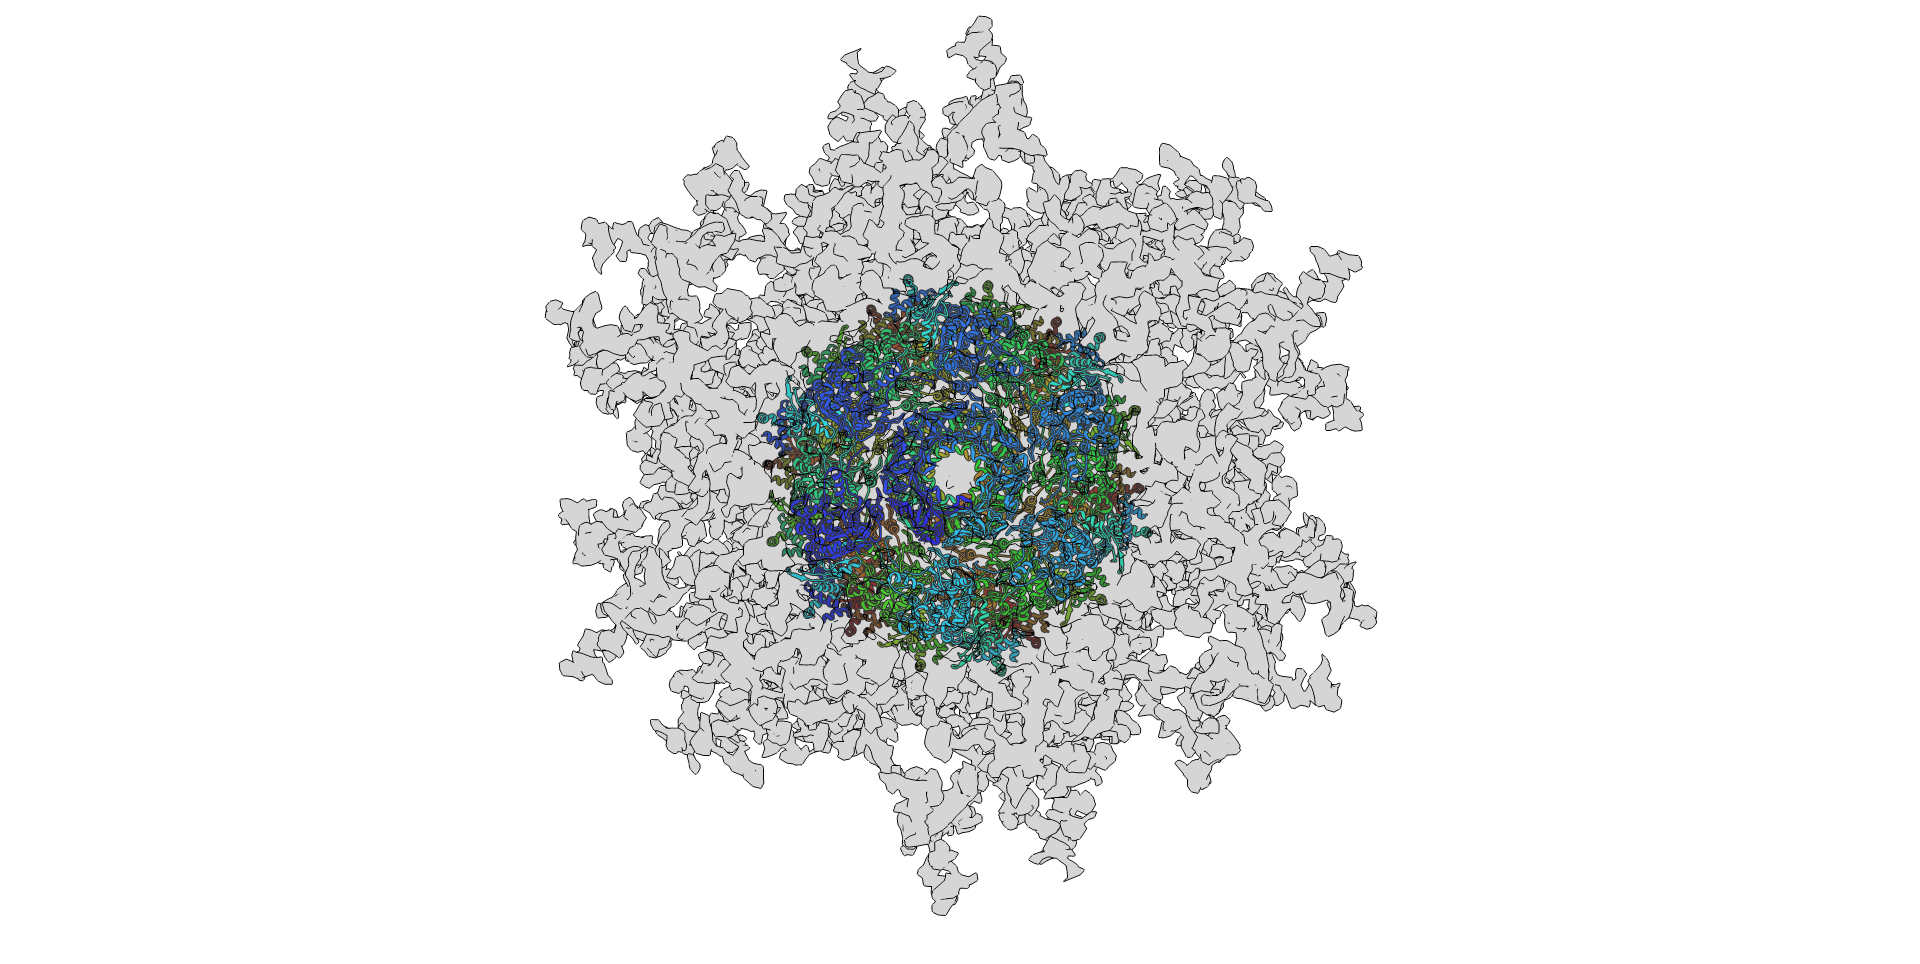
\includegraphics[width=0.6\textwidth, trim={55 0 55 0}, clip]{/Users/joehealey/Documents/Warwick/PhD/Thesis/chapters/intro/img/t6ss_distal_grey_flat_top.png}}} \\
     \end{tabular}
        \captionsetup{singlelinecheck=off, justification=centering, font=footnotesize, aboveskip=5pt}
        \caption{}
        \label{t6ss2}
        \end{subfigure}%
}\vfill
    \hbox{%
        \begin{subfigure}[t]{0.58\textwidth}
            \centering
            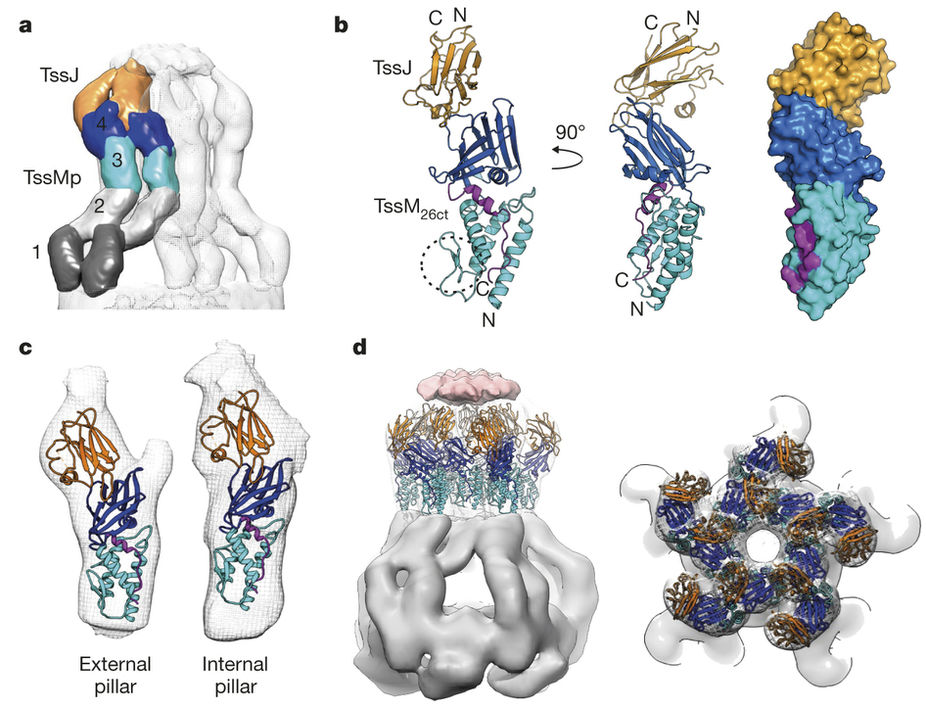
\includegraphics[width=\textwidth, trim={325 -100 0 360}, clip]{/Users/joehealey/Documents/Warwick/PhD/Thesis/chapters/intro/img/t6ss_tmc.jpg}
            \captionsetup{singlelinecheck=off, justification=centering, font=footnotesize, aboveskip=5pt}
            \caption{}
            \label{t6ss3}
        \end{subfigure}%    
  }\cr
}
\vfill
	\captionsetup{singlelinecheck=off, justification=justified, font=footnotesize, aboveskip=5pt}
	\caption[Type VI Secretion System Structures]{\textsc{\normalsize The structures of resolved components of the Type VI Secretion System.}\vspace{0.1cm} \newline \textbf{(A)} The EM density for the proximal and distal ends of the pre-contraction Type VI secretion tube. Figures were reproduced independently from the deposited data under EMDB-3878 and 3879 from \cite{Nazarov2017}. The density shows the spike complex and a distal cap like structure as well as the atomic architecture of the sheath. \textbf{(B)} Top left - a bottom view of the proximal end of the tube (spike toward the viewer). Top right - a slice through the centre of the tube, demonstrating well the dodecameric spokes in different planes. Middle bottom - a view from the top of the cap-like protrusion density. All also reproduced independently from \cite{Nazarov2017} EMDBs 3878/3879. \textbf{(C)} The 12 \AA{} map of the membrane complex of the system, with a TssM/J complex fitted in to the upper arches. Adapted and reproduced from \cite{Durand2015}.}
	\label{t6ss_structure}
\end{figure}

\clearpage

The T6SS is broadly divided in to approximately 4 structural complexes - a contractile tube (one could make the case that the spike complex forms a 5th component), a baseplate complex, a transmembrane domain, and associated soluble proteins. As a contractile tail system it, of course, exhibits a pair of concentric tubes, the inner of which is tipped with a spike complex, as with the other systems discussed so far. The inner tube is comprised of Hcp (``Haemolysin coregulated protein") hexameric toroids; Hcp being the ortholog of gp19/Afp 1 \& 5. The Hcp tube is approximately 80 \AA{} in outer diameter, with an inner lumenal diameter of roughly 40 \AA{} \citep{Mougous2006a}. Multiple crystal structures of Hcp orthologues and paralogues have been solved, and reveal the same overall gross architecture, though there is often some flexibility in the secondary structure and even more so in sequence. The inner tube appears more similar to that of R-type pyocins and the PVCs as it doesn't exhibit a helical turn, instead just being direct stacks of Hcp \citep{Silverman2012a, Mougous2006a, Osipiuk2011}. It was originally thought that Hcp itself was a secreted molecule, though without a known function, though it is now realised that the Hcp proteins may dissociate when puncturing in to the interior of another cell, and the filament of the tube is exposed to the extracellular environment during contraction. Thus, any dissociated Hcp monomers are essentially secreted `inadvertently', though this could obviously not be determined in the early experiments. In the T6SS of \emph{Edwardsiella tarda} it was also observed that the VgrG spike protein is secreted, but if either \emph{Hcp} or \emph{VgrG} homologues were knocked out, neither could then be detected in the supernatants of T6SS$^+$ cultures. The generally accepted, and likely, explanation for this is that Hcp tubules only assemble and secrete/puncture through the membrane if first polymerised off the VgrG baseplate hub analogous structure, as is the case in the T4 phage. Similarly, VgrG can only be detected in supernatants if Hcp is present to form the tube to which VgrG binds, and then is carried across the cell envelope by `riding' the tube out of the cell \citep{Pukatzki2007, Zheng2007, Hachani2011}. High resolution microscopic studies with the help of fluorescent constructs have been able to demonstrate that multiple T6SS complexes can be carried by a cell at once, and the tube complexes can extend many hundreds of nanometers, deep in to the cytosol of the cell - even reaching the opposite cell envelope \citep{Nguyen2018, Chang2017}.

Unlike the other systems mentioned up to this point, the exterior sheath of the T6SS differs quite substantially in structure, despite still forming a contractile system. As can be seen in the upper right panel of \vref{t6ss2}, the outer sheath is actually a dodecameric toroid, comprised of 2 different proteins: TssB and TssC. Type 6 secretion proteins have been given alphabetic nomenclature preceded by ``Tss" (Type six subunits), as such, the outer 2 sheath proteins for example, are termed TssB/C, and though unrelated, would be the structural orthologues of gp18 in T4. TssB is a smaller protein of around 18 kDa, and TssC comprises the bulk of the tube at $\approx$55 kDa. Together they form an alternating dodecameric ring which is approximately 240 \AA{} across in the extended state and 290 \AA{} in the contracted form, with an inner diameter of 80\AA{} before contraction, and approximately 110 \AA{} post-contraction (in the \emph{V. cholerae} T6SS structure) \citep{Cascales2012, Wang2017, Kube2014a}. If one were to think of the ring as an analog clock face, a TssB monomer would occupy all the odd numbers, and a TssC monomer would occupy all the even positions \citep{Kube2014a}. In the extended form, the sheath has a 38 \AA{} rise, and a 23.6$^{\circ}$ twist, and this shifts to a 15.8 \AA{} rise and 29.4$^{\circ}$ twist after contraction \citep{Wang2017}. Both subunits appear to contribute to protrusions around the exterior of the tube which form a left-handed helical series of ridges. This is not a trivial observation either, as this is the opposite handedness to the T4 phage tail. Such a dramatic rearrangement in structure further underscores the hypothesis/observation that T6SS outer sheaths are unrelated in origin to T4 phage \citep{Kube2014a}. As is the case with the PVCs and Afps, one of the most conserved proteins appears to be a ClpV AAA+ family ATPase. These are typically protease enzymes which take their name from being ``ATPases Associated with various cellular Activities'', and are a group of enzymes/chaperones which are able to cause conformational changes in an enormous variety of cellular proteins \citep{Hanson2005}. It has been demonstrated that the ATPase is not entirely essential for T6SS function (at least in \emph{V. cholerae}) but its role has recently been determined to be in recycling of the tube after contraction, utilising these sheath protrusions, ameliorating some of the significant cost to the `cellular economy' of building such an enormous and complex structure. Consequently, the ATPase is required for repeated synthesis and discharge of the same T6SS complex, though cells are perfectly capable of continuing Type VI mediated secretion, though an entirely new T6SS must be generated, essentially becoming `single use' \cite{Basler2015}. The ATPase itself forms a hexameric ring, and interacts with an $\alpha$-helix near the N-terminal of TssC using its central pore, and dissociates it from TssB only in the contracted state, this causes the outer sheath to `disintegrate', freeing up the subunits for recycling \citep{Costa2015}; in the extended conformation, the helix is obscured preventing premature depolymerisation. The presence and role of the ATPase within Afp and PVC operons remains a mystery, since there is less rationale for a need to recycle the components which are released from the cell completely. Due to its high level of conservation and readily identifiable domain family, despite not being entirely essential, ATPase presence and recycling is now considered a hallmark of Type VI secretion \citep{Nguyen2018}.

Sitting atop the tube complex is a PAAR spike-tip protein and  VgrG spike complex which is homologous to the gp27-gp5 complex of T4, though lacks the lysozyme domain (a seemingly common `deletion' outside of T4). Interestingly, in the Type VI, due to the huge diversity of operons in the vast number of sequences studied to date, there is now evidence that in certain cases the T6SS also employs so-called ``evolved VgrGs" \citep{Pukatzki2007, Suarez2010, Hood2010, Cascales2012}. A slightly clumsy term perhaps, but the premise is that different VgrG spikes have, in effect, acquired domains for alternative enzymatic functions that can exert an effect on the target cell once they're translocated in to the interior. By doing so, the Type VI is able to deliver a `double whammy' of delivered effectors from within the tube lumen, as well as a functionalised `warhead'. Clearly, the VgrG is not just a wedge with which to separate the cell envelope, and similarly, the  PAAR repeat proteins which sharpen the VgrG apex, are more than simply structural. Discussion of these proteins has been left until now, despite there being orthologues in most of the structures discussed so far \citep{Sarris2014}, as the T6SS appears to have among the most interesting collection of these tiny proteins, and some of the better characterised experimental data. PAAR proteins take their name from ``Proline-Alanine-Alanine Repeats", which in concert with a coordinated metal atom, confer on the protein a triangular pyramidal shape. The T4 phage analogue of this protein is gp5.4, and they were initially identified for T6SS by Schneider et al., by examining all small proteins (\textless 23 kDa) associated with gp5 bearing genomes \citep{Shneider2013}. Amazingly, in many cases these PAAR spikes present a single amino acid side chain at the tip, making it as sharp as just a single atom or two (e.g in the PDB ID 4JIV, a lysine sidechain sits at the apex). This is not just a simple honing process to improve the T6SS puncturing efficiency however, the PAAR spike tip proteins have been shown in at least 2 studies to be essential for T6SS function \citep{Shneider2013, Cianfanelli2016}. The claim was made earlier that PAAR repeat proteins are more than simply structural, and indeed that is the case. A growing body of evidence has been able to identify a number of toxins which are bound to the PAAR spike tip, in a similar fashion to those associated with VgrG \citep{Hachani2014, Ma2017}. \cite{Cianfanelli2016} additionally showed that VgrGs and PAAR proteins are not completely interchangeable, with certain combinations having a clear preference for one another, and moreover they had a specificity for the types of effectors they carried, to the extent that they define distinct `versions' of the Type VI. All in all, this means that the Type VI, as well as being a `loaded needle' can also act like a `poison arrow', discharging a lethal tip, upon injection.

The baseplate complex of the T6SS has not been well studied to date, but is suggested to continue the homology to that of phage T4. The baseplate is known to comprise the proteins TssE, F, G, and K. TssK forms a trimer, and has had its structure resolved recently. Unusually, the protein loosely resembles a tail fibre like structure, with a `head` and `shoulder` region, connected by a neck/shaft-like region, though this has yet to shed any light on an actual role \citep{Desmyter2015, English2014}. It has been suggested, that the baseplate is formed of subcomplexes, akin to the baseplate wedge complexes seen in \vref{wedgeformation}, and most likely follows a hexameric symmetry. A homolog of gp25, a protein which interfaces the spike hub complex and the tube proper in T4 has been identified in a Type VI locus from \emph{E. coli} corresponding to TssE, which is essential for tube biogenesis \citep{Nguyen2018, Brunet2013, Leiman2009}. TssF and G are further proposed to form a complex reminiscent of gp6-gp53, which do form a significant part of the wedge assembly and would fit with the hypothesis that the baseplate will also exhibit 6-fold symmetry \citep{Nguyen2018}. Attempts to determine this by stoichiometry analyses have been frustrated so far however, and there is conflicting information \citep{Nguyen2018, Nazarov2017}. It will simply be a matter of time before structural data of sufficient quality is obtained to answer this once and for all, and given the intense interest and rapid pace of research in the area in the last decade or two, it seems unlikely that it will be much of a wait.

The membrane bound components of the T6SS include TssL, M and J. TssL is present in the inner membrane, and TssJ is situated at the periplasmic face of the outer membrane. TssM is a large protein (1100 residues) and has been shown to interact with both TssL and TssJ, meaning that its most likely configuration is spanning the periplasmic space to bind the inner and outer components together, though any conclusive structural data is still lacking \citep{Zheng2007, Ma2009, Felisberto-Rodrigues2011, Nguyen2018}. Some gross architecture was uncovered in 2015, when a 12 \AA{} map of the membrane complex was determined \citep{Durand2015}. The complex consists of 5 `pillars' and a TssM-J complex was able to be fitted in to the density to reasonable accuracy, though much of the structural information for the inner membrane proximal region is still lacking. Interestingly, this means that the T6SS displays 3-fold (VgrG complex), 6-fold (Hcp tube), 12-fold (outer sheath) and 5-fold (membrane complex) symmetries, which is unusual compared to the other systems studied so far, which are all 3 or 6-fold. There is some suggestion that this 5-fold symmetry may be an aberration however, since the recently resolved TssA protein, a putative sheath cap, was shown not to bind to C5 complexes, and conferred a 6-fold symmetry to the membrane complex via displacement \citep{Zoued2016}. As with the baseplate, it is unlikely that the architecture of the membrane components will remain a mystery for long.


In summary, the current operating hypothesis is that the T6SS has an overall architecture where the contractile sheath and spike complex is surrounded in the membrane space by a sort of pear-shaped, buttressing cage of struts. This membrane complex scaffolds the central tube core of the system, and complexes with the baseplate at the interface of the cytosol and inner membrane, though structural data relating to this interaction is still missing. 12 of the 13 identified `core components' have been localised, if not structurally resolved, on at least a preliminary basis. The 13th, the ATPase, is a known cytosolic protein, which it needs to be to exert its disassembling role.


\subsubsection{Of PVCs and their extended family}
The known role, based on the earliest experiments on the PVCs, is as toxin delivery systems \citep{Yang2006}. However, as seen in the Type VI Secretion System, contractile tail structures are not limited to this function. In recent years there have been a number of unusual related systems discovered which demonstrate extremely diverse ecological roles aside from just virulence/lethality. This section will explore some further examples of enigmatic `second cousins' of the PVCs. Many of these apparatuses are not well characterised and this is unlikely to be an exhaustive list, but these are some of the more unique and better studied examples which have evidence beyond simply matching in database queries like BLAST.

\myparagraph{In \emph{Pseudoalteromonas luteoviolacea}}\label{mac}
\hspace{-.1cm}As alluded to in the last paragraph, until very recently, `tailocins', Afps, and the PVCs were the only known examples of `secreted' caudate structures (not including phage) - and all of them have been observed to exert a lethal effect in, in one form or another, against the targeted cells. In 2014, this changed, as Shikuma et al. published structural data of a remarkable contractile complex produced by the marine bacterium \emph{Pseudoalteromonas luteoviolacea}. Termed the ``Metamorphosis Associated Contractile" Structures or ``MAC" complexes, they observed that these incredible assemblies were the cryptic causative agent that drove the differentiation of the larvae of the marine tubeworm, \emph{Hydroides elegans}, in to its juvenile form \citep{Shikuma2014}. This discovery was astounding for 2 particular reasons. Firstly, their discovery represents the first example of a beneficial interaction between a type of contractile structure, and a target organism. Prior to this finding, it had been observed that many marine organisms respond to bacterial associations, but the underlying mechanism(s) had not been uncovered \citep{Hadfield2011}. Shikuma and colleagues were able to demonstrate a differentiable phenotype with purified MAC complexes, unambiguously confirming its role. When they probed the structure of the MAC complexes, the second astounding discovery was made. Not only are the MAC complexes caudate contractile structures, but they are actually formed from an interlaced hexagonal array of tail tubes, which are `secreted' (released from the cell by lysis), and, in effect, form a kind of `bed of nails'. The tails are all `up-ended', such that the spikes face away from a substrate they are attached to, and the tails essentially interlock their arms, with 6 tail-fibre like proteins from each tube interacting with the 6 adjacent tubes, and each tube therefore contributes 6, and receives 6, points of contact with its neighbours.

In order to metamorphose, the tubeworm must lie on this bed of contractile nails, at which point contraction is triggered (by an as yet undetermined mechanism), and differentiation factors are delivered in to the larval worm. These differentiation factors still remain to be concretely identified, but in a followup paper, Shikuma and colleagues were able to narrow the possibilities down to a short stretch of sequence ($\approx$8.2 kb), comprising 6 proteins sequences, in close proximity to the MAC operon, which were able to induce Mitogen Associated Protein Kinase (MAPK) based signalling cascades \citep{Shikuma2016}.

\myparagraph{In Amoebophilus asiaticus}\label{cis}
\hspace{-.1cm}More recently, another example of a MAC-like structure was structurally elucidated, but this time in an amoeboid symbiont, \emph{Amoebophilus asiaticus}. Unlike the MAC complex, this complex which the authors identify as an arrayed T6SS (``Type VI Secretion System$^{subtype IV}$"), is purely membrane associated. Nevertheless, it still resembles an interlocked `bed of nails'. No obvious density could be imaged for any tail-fibre filamentous network like that observed in the MACs, though its possible that being embedded in the membrane like the T6SS, means that the collar/membrane complex region could be held in tight register by other means \citep{Bock2017}. The structure forms a tightly packed hexagonal array, putatively joined at the baseplates at the cytoplasmic face of the inner membrane, though the complexes are somewhat smaller. In the MACs, it was not uncommon to see arrays of 100 tail tubes, whereas the average for these T6SS$^{IV}$s is only 8.

However, \cite{Nguyen2018} observes that this structure appears to be a `stunted' T6SS, as the tube is much reduced in length. Some other curiosities include the fact that it contains a tape measure protein, which a canonical T6SS does not, it has no known effectors, and is not recycled by an ATPase - most of which are considered hallmarks of a `true' Type VI. Thus, Nguyen et al disagree with the authors that this represents a new type of T6SS, and instead suggest it more closely resembles a membrane bound Afp. The criticism from Nguyen et al. is probably well founded, as even the authors note that the system is much more closely related to Afps/MACs and a similar complex in another intracellular mutualist, \emph{Cardinium hertigii}, and lacks any real similarity to the T6SS at the sequence level.

A role for the \emph{A. asiaticus} complex has not been determined fully, though its similarity to the \emph{C. hertegii} structure, and the fact that both organisms share an intracellular lifestyle is thought to suggest they play a similar role. The \emph{C. hertegii} complex is discussed in the next section.

\myparagraph{In \emph{Cardinium hertegii}}
\hspace{-.1cm}Very little is known about the structure of the Afp-like island that \cite{Penz2012} identified in the genome of the endosymbiont (of parasitic wasps) \emph{Cardinium hertegii}. However, a putative role has been suggested. Bacterial symbionts of insects are well known, and  perhaps the best understood example is \emph{Wolbachia}. These symbionts are capable of exerting large scale physiological and developmental effects on the host \citep{Hedges2008, Oliver2003}. One of the best studied effects is ``Cytoplasmic incompatibility". This has serious reproductive consequences; when a male harbouring the endosymbiont reproduces with an uninfected female, the embryos become non-viable and die very early in gestation. By doing so, a fitness cost is conferred against uninfected individuals thus promotes the survival of the endosymbiont \citep{Werren2008}.

In \emph{Wolbachia}, a Type VI Secretion System is responsible for mediating cytoplasmic incompatibility, suggesting that factors derived from synthesis inside the cytoplasm of the endosymbiont are important causative agents of this phenomenon, and thus they must be translocated to the cytosol of the host. \cite{Penz2012} observed that there are no known secretion systems in \emph{C. hertegii}, but they do harbour 16 Afp-like genes, though fragmented in to 5 different loci, rather than a single cassette. It is not known whether there are membrane-bound associated proteins which would be able to present these Afp-like genes in a more `conventional secretion system' form, though this seems probable, since it is unlikely that there is much need to secrete a whole tailocin like structure, when the bacterium is already within the cell. At present, there are no known toxins or other substrates for the putative secretion system either, but this does suggest another non-pathogenic utility to contractile tail structures. Furthermore, given the diverse pathways intracellular symbionts are known to be able to manipulate, it seems likely that this may represent another general purpose secretion system \citep{Werren2008}.

%\myparagraph{In \emph{Streptomyces endus}}
% \cite{Ogata1982}

To summarise, it's evident that caudate structures appear to by widespread in all bacterial species, potentially somewhat `enriched' in marine species, and are capable of serving a wide variety of ecological functions. \vref{structure_diagram} shows a schematic overview of the similarities between these structures and their targets, collecting all the information of the past sections.

\begin{landscape}
\begin{figure}[p]
\thisfloatpagestyle{IHA-fancy-style}
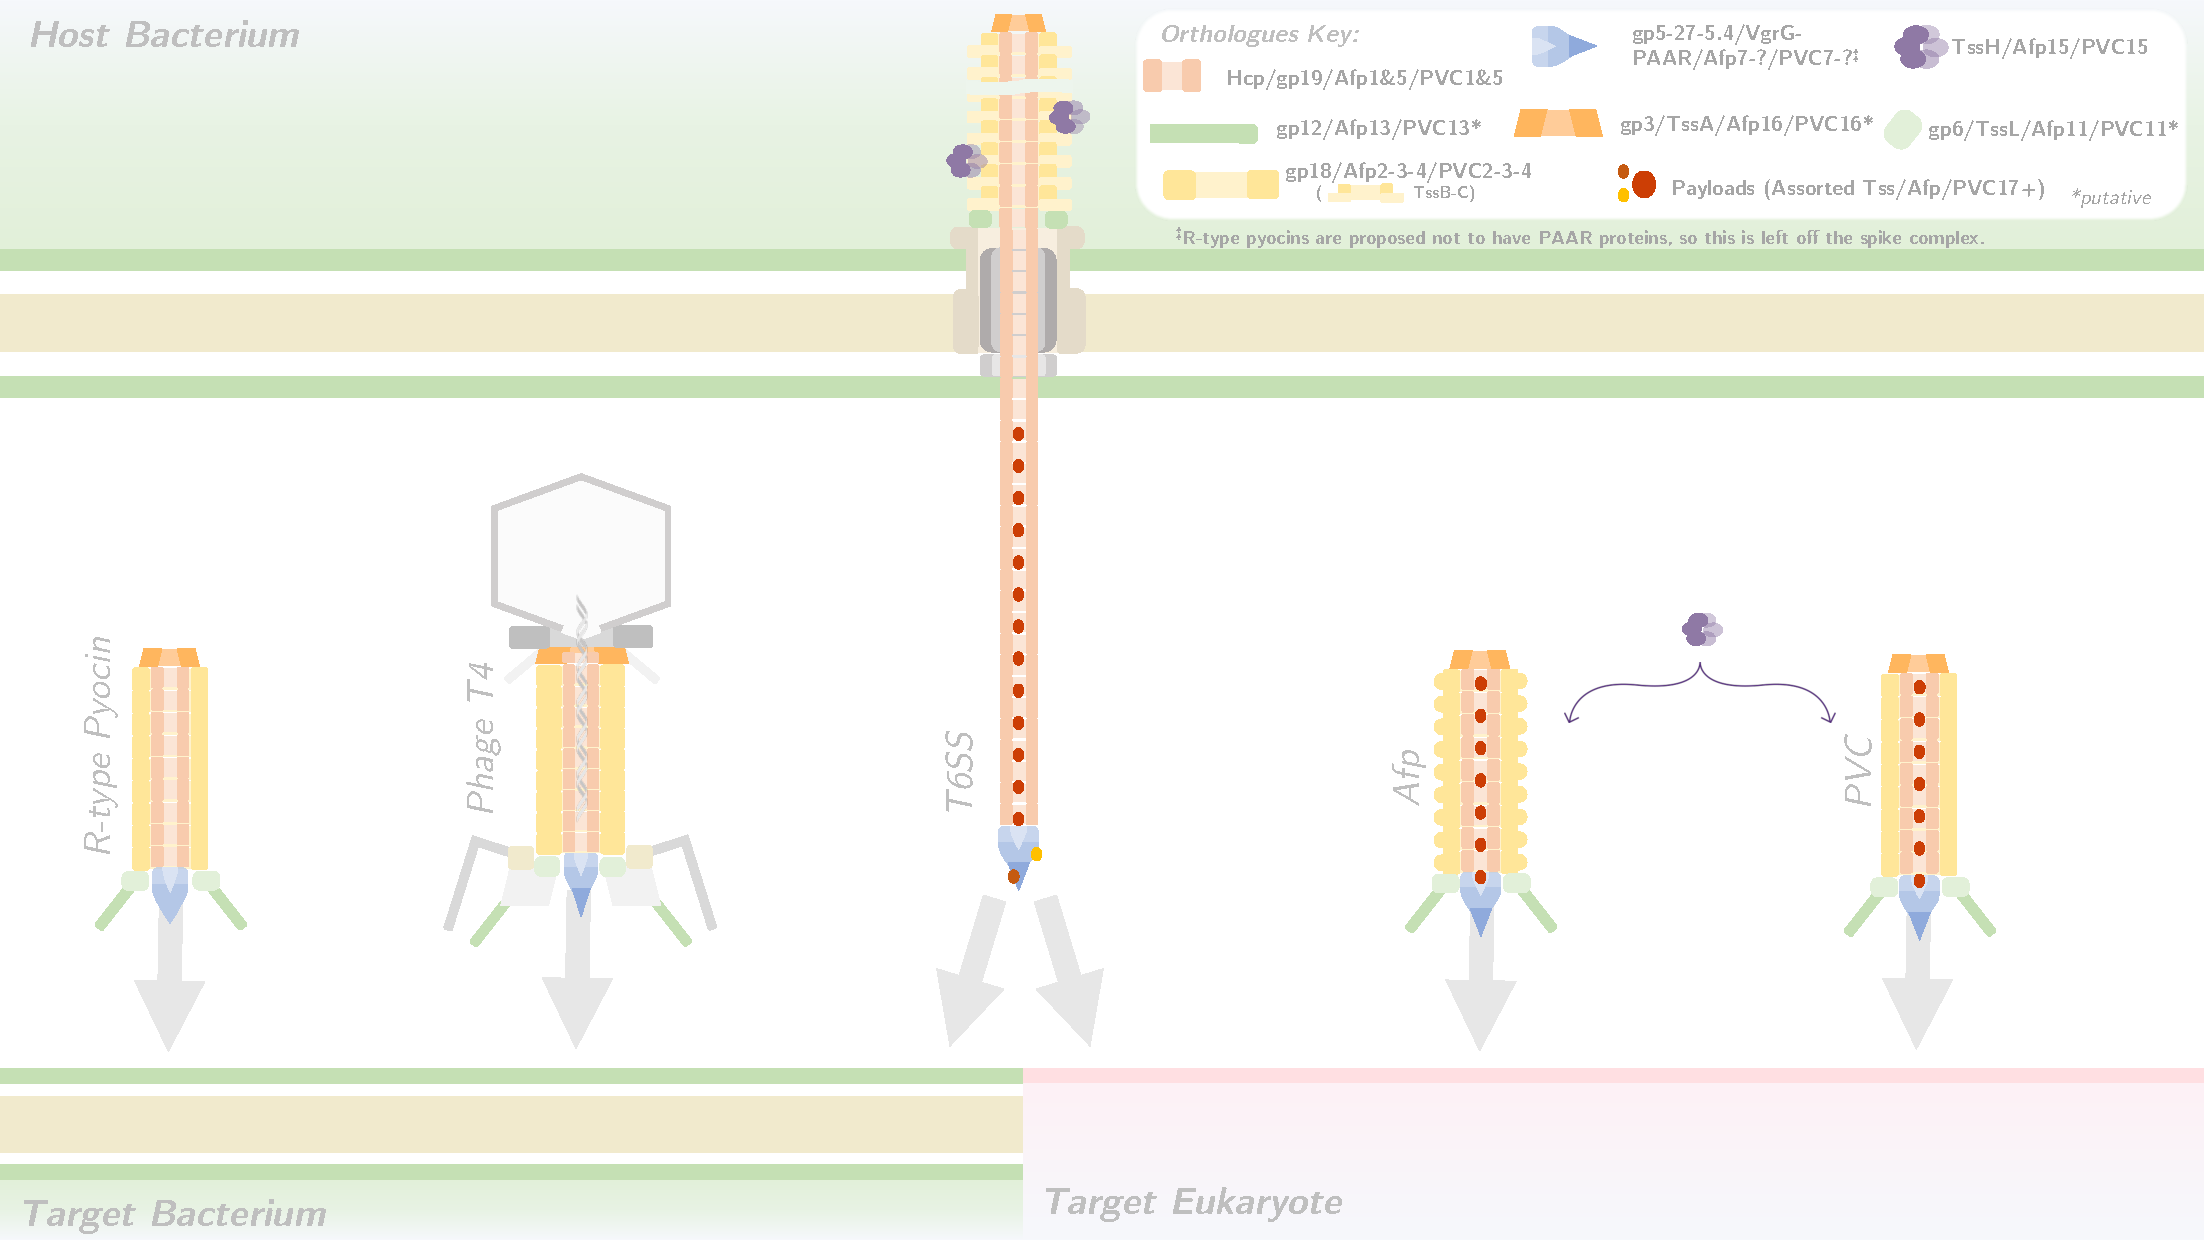
\includegraphics[width=\linewidth]{/Users/joehealey/Documents/Warwick/PhD/Thesis/chapters/intro/img/Structure_Comparison.pdf}
	\captionsetup{singlelinecheck=off, justification=justified, font=footnotesize, aboveskip=5pt}
	\caption[Schematic of conserved caudate architecture]{\textsc{\normalsize Schematic of conserved architecture in various caudate structures.}\vspace{0.1cm} \newline A diagrammatic comparison between the conserved components of PVCs and other caudate structures discussed in this introduction. The inset key depicts structural orthologs, though they may not be ancestrally related. Neutral/gray colours identify proteins which are not shared between structures. Items in the key with asterisks are putative homologues. A question mark indicates that a homologous structure has been identified, but the protein is not yet known. Not to scale.}
	\label{structure_diagram}
\end{figure}
\end{landscape}
\newpage

\subsection{Mechanism of Action}\label{mechanismofaction}
The actual mechanism of contraction has been the subject of significant debate and speculation in recent years. It has been generally accepted that the pre-contraction state of the tube complex represents an energetically tensioned system (meaning that the often seen of references to this conformation as `relaxed', is in fact, the exact opposite), and the prevailing hypothesis has been that the conformational change in the outer sheath proceeds in a wave-like fashion from the proximal baseplate, toward the capsid, and is driven by solvation free energy gain \citep{Brackmann2017, Kube2015a, Kube2014, Moody1973}. 

As the pre-contraction state is therefore an energetically unfavourable conformation, it begs the question of how contractile tail structures are able to be assembled seemingly against the laws of thermodynamics. While there is still no definitive answer to this, despite the wealth of data now available, the generally accepted mechanism is that the baseplate is produced first, in a static form (not changing in the contraction process), and serves as a `nucleation site' and a sort of intrinsic chaperone, allowing the first tier of the tube to polymerise off it. In effect, the baseplate is analogous to the pin in a mousetrap or a grenade, holding the conformation of the first tier in its a `locked' and tensioned state. The logic then follows that the tensioned tier 1 of the tube acts as an `auto-chaperone' allowing further tensioned forms of the tube hexamers (or dodecamers in the case of T6SS) to polymerise off it, also in a tensioned form \citep{Kube2015}.

For the T4 phage, it is now understood that the contraction of the tube is triggered by conformational changes transduced through the tail fibres, leading to large scale rearrangements in the baseplate. A contractile trigger mechanism for the Type 6 remains to be discovered, though the cryptic `antennae' that can be seen in the right panel of \vref{t6ssEMs}, may suggest that the T6SS is prompted to contract in a similar manner, which would also allow the cell to sense when a target is in close proximity, such that the T6SS is not discharged aberrantly, causing significant cost to the cell to regenerate. 

The contraction process is an enormously energetic process as a result of the release of the sheath tension. Not only is there a lateral translocation of the inner tube to provide the eversion, but the helical nature of the outer sheaths also applies a rotational torque to the sheath, quite literally drilling it in to the target cell envelope \citep{Kube2015}. This leads to some very impressive statistics. \cite{Wang2017a} calculate that for contraction of a ``1 \um{} long sheath, composed of 260 rings, [the sheath] would push the inner tube by 420 nm and rotate it by 4.2 turns [...]. The overall amount of energy released during a single sheath contraction could be close to 44,000 kcal mol$^{-1}$". \cite{Vettiger2017} report that the entire contraction of the sheath occurs in just a couple of frames, even at 500 frames per second, and they conclude that the contraction speed is therefore \textgreater 800 nm per millisecond. The Type VI is  something of a special case given the lack of restriction on tube length, but \cite{Wang2017a} calculate, on a per-subunit basis, that ``the free energy gained during contraction is 28.5 kcal mol$^{-1}$ subunit$^{-1}$, more than 9.1 kcal mol$^{-1}$ subunit$^{-1}$ calculated for [the] R-type pyocin". Exact contraction kinetics have not been observed for the other contractile mechanisms, but even the extrapolation here demonstrates that a significant amount of energy is expended by contractile machines to traverse these membranes \citep{Brackmann2017}.


\subsection{The \emph{status quo} of PVC genetics}
With the superficial resemblances to analogous structures covered, this section will briefly highlight the state of knowledge about the gene modules within the PVCs specifically when this project began. This provides the `jumping off point' for the upcoming Chapter, where the roles for many of these genes were probed further bioinformatically.

\subsubsection{The PVC tail tube and sheath}
As mentioned in previous sections, the tube and sheath components of the PVCs have long been among the best annotated genes within the operons, though this does not necessarily say much. Typical annotations, for instance from the first annotation of the published \emph{P. asymbiotica} ATCC43949 genome, for the ``LopT" PVC operon include ``phage tail sheath" and ``phage tail region" proteins. Belying the diversity of the PVCs which this thesis will continue to unpick, however, many of the operons still only picked up ``conserved hypothetical protein" annotations, even for these proteins. Of some approximately 350 CDSs made up from 16 operons identified in 3 genomes (see \vref{pvcvariants}), around 250 of them had no functional information whatsoever, and those that did were almost exclusively the cognate toxins and some tube proteins. Furthermore, in the TT01 genome, every single locus for every single PVC operon had the descriptor ``hypothetical protein", with no useful functional annotations whatsoever.

Nevertheless, with further inspection via BLAST and other tools, a good understanding of much of the PVC structure was able to be elucidated by \cite{Yang2006}. The phage tail tube proteins were unambiguously identified, though this wasn't true for the whole operon. Some additional observations could be made, including the deletion of a sheath protein in 3 operons. This raises questions about why the PVCs maintain 2 inner sheath and up to 3 outer sheath proteins, when at least one is evidently non-essential (assuming all PVCs are fully functional), and other caudate structures typically do not.

\subsubsection{The spike complex and baseplate}
The original genome annotations tell a similar story for the putative baseplate complex. What has subsequently been identified as the PVC's VgrG spike protein homologue, has only previously been annotated as hypothetical. Other structural components of a putative baseplate were detected however, with several operons displaying annotations for ``phage baseplate assembly proteins", ``similar to baseplate protein gp25". Though once again, the underlying variability in the PVCs means that a number of operons were left with uninformative annotations still. It is likely that much of the `dark matter' in the middle of the operon contributes to the baseplate apparatus, but with little to no orthology to anything previously detected in the databases.

\subsubsection{The operon core}
What is being termed here as the `operon core' describes a number of single copy genes located in the centre of the operon, which appear relatively conserved, and potentially have important non-structural roles. Though there are only a couple of useful annotations for this region, the \cite{Yang2006} paper was able to identify some compelling orthologues. Firstly, a gene which putatively has a role in transcript regulation resides in approximately locus position 10 (though this varies if operons have deleted upstream genes of course), but little else is known of its role, and the sequence identities are low \citep{Waterfield2009}. Immediately downstream of this is an unknown protein, with no functional information whatsoever.

The next gene, typically in locus position 13, is the putative tail fibre gene for the PVC complex. In the PVClumT operon of strain ATCC43949, this was attributed adenoviral tail fibre orthology. This is unusual, given the hypothesised bacteriophage origin of the structure, and there are no other known examples of this non-phage-like sequence similarity in other caudate structures, making the PVCs potentially unique. It has been demonstrated experimentally that the PVCs only exert toxic effects against eukaryotic targets (insect haemocytes), and have no antimicrobial activity whatsoever. It is possible that the reason for this that the PVCs have evolved anti-eukaryotic target recognition tail fibres, and thus they no longer bind to/work against prokaryotic targets. These unusual tail fibres are explored much more extensively in \vref{tailfibres}.

Positions 14 and 16 in the operon core also elaborate proteins with no readily apparent functions. The best hypothesis for these proteins, based on the experimental data and synteny with the \emph{Serratia} Afp, from the Hurst et al. experiments, is that they are the PVC equivalents of tape measure proteins and some kind of tube terminator or cap \citep{Rybakova2013, Rybakova2015a}. \vref{structbioinfo} speculates on these proteins a little further.

Lastly, locus 15, despite not being well annotated in the originally available genomes, is readily identifiable as a AAA+ ATPase, like that of the T6SS (though from a distinct phylogenetic family \citep{Frickey2004}). Despite its ease of identification, there is currently no further experimental information available to suggest a role as covered in section \vref{t6ss}. The main hypothesis to date had been that the ATPase maybe served as a `loading pump', passing the PVC payloads in to the lumen of the tube, though this is purely speculation.

\subsubsection{The hypervariable payload region}
Finally, a hallmark of the PVCs which has been alluded to a few times in this introduction already, is the hypervariable toxin payload region. As there are multiple operons for each PVC, they each carry at least 1 unique toxic effector. This has not been observed with any other related structures, with the partial caveat of the fact that Type $x$ Secretion Systems are known to have various substrates, but they are not necessarily encoded \emph{cis} to the system itself. The carriage of \emph{cis} encoded toxins is true for the Afps as well, which once again highlights the similarity between them and PVCs. Similarly, while there are no shortage of caudate structures which have been identified in the literature, in studies like \cite{Sarris2014}, the PVCs remain unusual for this particular feature, and therefore potentially do not entirely fit in to the classifications others are attempting to apply to them.

The toxins encoded in the PVC loci are typically easy to identify, and have been reasonably well annotated, in part because they generally appear to be effectors which are already well known bacterial toxins from other systems. Pnf, for example, is and unequivocal orthologue of cnf1 from \emph{E. coli}, and was annotated as such in the original ATCC43949 genome. Similarly, the lopT operon in the same genome, harbours 3 different toxins, all of which have been seen in other instances. The lopT toxin itself takes its name from the yopT cysteine protease class of toxins in \emph{Yersinia}, an rtxA toxin is also present which is named for the family of toxins to which it belongs (``repeats-in-toxin"); a family that is well represented in other organisms, such as \emph{Vibrio} \citep{Lin1999}. Lastly, it also harbours a TccC domain protein, which are the toxic components of the Tc toxin complexes, which are actually elaborated by \emph{Photorhabdus} itself, separately, and were recently structurally resolved \citep{Bowen1998, Meusch2014} and are yet another staggeringly impressive toxin delivery mechanism of the bacteria. Nevertheless, following the trend in this section, not all operons were given useful or informative annotations, even for the toxins.


\subsection{PVC myths}
Despite the increasing wealth of information appearing, there are several papers which, in their attempts to group the PVCs with other structures, appear to come to spurious conclusions, and this section will briefly draw attention to these.

Firstly, \cite{Zhang2012a}, suggest that the ATPase which is distinctive within the PVCs has a role in cleavage/delivery of toxin molecules that is in some way separate from that of the PVC structure. There is little to no experimental evidence for this, and the majority of the paper disregards the actual syringe complex which is arguably the most important component. They do suggest that the ATPase may have a role in recycling the PVCs, as it has been shown to in the T6SS. However, as all the evidence to date points to the release of the PVCs, to act at a distance in a `torpedo' like fashion, there appears to be no evolutionary need/advantage to recycling the structure. That said, two possible explanations for its persistence, if recycling is its actual role, are that it may be vestigial, though this seems unlikely given the level of conservation. Given the fact that these ATPases are defined by their roles in various cellular pathways however, it could be that sufficient selection pressure to maintain the ATPases is being exerted based on their activity outside the PVC operons \citep{Iyer2004a}. Alternatively, the ATPase may recycle the tube subunits continually so that they do not build up unnecessarily inside the cell, before mature PVCs are ready to be deployed `in anger'. Since so many more of these proteins are required per syringe, its possible that they're made in significantly higher proportions, and to offset the metabolic cost of building such a structure aberrantly, they are being turned over continually to replenish cellular concentrations of amino acids and other substrates.

They speculate that the N-termini of the toxin effector molecules contain a distinctive metallo-peptidase domain/activity, though the paper is not clear on what sequences were used to arrive at this conclusion. From our own studies (as yet unpublished), it has been demonstrated that the N-termini of the toxins for several PVC effectors have a stabilising/chaperone-like role, possibly with a syringe loading signal. However, it is more or less impossible to construct a meaningful multiple sequence alignment for all but the most closely related effectors, much less to define a characteristic domain structure for all PVC toxins, which calls in to question some of the conclusions of the paper, at least for the sequences they are attributing to PVCs.

Despite being an otherwise excellent review, Kube and Wendler make the statement that  PVC sheath proteins are most like T4 sheath proteins, but pyocin proteins are most like phage P2. This appears only partly true however \citep{Kube2015}. \vref{structbioinfo} examines this further, but it appears that actually only one of the sheaths (the inner) is T4 like, whereas the outer is pyocin- (and therefore P2) like, also resembling the T6SS. In the same paper, the authors also make the statement that the Afp cluster lacks any lysis systems, which are seen in phage and pyocins. While it is true that evidence for lysis-based release of the PVCs and Afps is scarce as the authors point out, the PVCs can often be found with lysis associated proteins. For example, downstream of the PVCPnf ATCC43949 operon, beyond the payload region, but on the same strand and in close register to the rest of the operon, several bacteriophage lysis proteins and lysozymes can be detected, though it is true that this cannot be said for all of the operons, at least at the present level of sequence identification. It seems the likely do harbour general lysis systems, though some of them may be comparatively enigmatic.

Similarly, though it is also an excellent study, the \cite{Sarris2014} paper makes many claims about the PVCs in attempting to group them with other ``Phage-Like-Translocation-Systems", though they appear to be only considering a single PVC example from \Plum{} (``Unit2"), and some of these statements may not hold true for all PVCs. One example of an erroneous claim is in their discussion of synteny conservation. While there is undoubtedly a great deal of synteny conservation, they state that the sheath proteins are typically located downstream of baseplate genes. It's not clear whether this is simply a syntactical or typographical error, but it's readily apparent, including from the figures in their own paper, that the reverse is true. Since they are basing a level of significance on these similarities for identifying similar structures elsewhere, this synteny rearrangement would potentially have consequences for how sequences are grouped and ancestry inferred. Another objectionable conclusion is their readiness to include many, potentially distantly related, operons in to this ``PLTS" family, without any actual consideration being paid to whether the operons harboured any payloads which are translocatable. This is important, as they identify R-type pyocins, which are non-translocating structures, as a separate `clade'. Thus, whether or not a candidate caudate structure should be considered more like an R-type pyocin or an Afp/PVC cannot be decided from sequence alone due to the huge diversity, and functional relatedness is therefore a key factor. Additionally, Sarris and colleagues also fall foul of the same observation as \cite{Kube2015}, in stating that there are no lysis proteins associated with PVCs. Had they considered more than one PVC example in their analysis, they may have observed that this doesn't appear to be true.

\section{Summary and Thesis Aims}
Despite this richness of data for related systems - the cumulative product of centuries of study - the picture is, perhaps unsurprisingly, still far from complete for the PVCs, being comparatively understudied. Their unique role as bacterial secretion systems that act at a distance means there is much left to be understood about what makes them different. This thesis attempts to tackle this in a number of ways:

\begin{itemize}
\item Firstly, an up-to-date exploration of the structural similarities and differences with the benefit of time and more advanced bioinformatics resources/databases versus the original description of PVCs can be found in \vref{structbioinfo}. This chapter aims to improve understanding of the poorly characterised genes for all the proteins in the operons, and generate hypotheses for testing in the lab and for future work.

\item Secondly, a phylogenetic study of the PVCs which attempts to shed light on the microevolution within the operons, examining the variability and loss of genes in this context, can be found in \vref{bioinformatics}. All the comparative genomic studies that have been covered in this introduction are keen to place the PVCs in a wider context, whereas an inward-looking study trying to better understand why so many PVC variants exist, and why they are so diverse has been lacking. 

\item Key proteins in the mechanistics of (at least) non-membrane-bound caudate structures are the tail fibres. They are responsible for triggering the contractile mechanisms, and also conferring the `target spectrum' that the structures are able to act against. For the PVCs, sequence similarities in these proteins were weak at the outset, though curiously, some were able to pick up annotations against Adenoviral motifs. \vref{tailfibres} explores the tail fibres in more detail, and represents possibly the first experimental studies of naturally occurring chimeric tail fibres.

\item \vref{regulation} explores efforts to understand the natural expression patterns of the PVCs, as well as attempts to heterologously clone and express the PVC operons. Experimental work to date had been conducted with a cosmid library, but there were several issues with this approach. The PVCs were still under the control of their native promoters, and this made them unstable and difficult to work with in the lab. A key question for this chapter, therefore, is to try and probe any population heterogeneity in how the PVCs are deployed naturally.

\end{itemize}


